\documentclass[10pt]{report}
\usepackage{geometry}                % See geometry.pdf to learn the layout options. There are lots.
\geometry{letterpaper}                   % ... or a4paper or a5paper or ... 
%\geometry{landscape}                % Activate for for rotated page geometry
%\usepackage[parfill]{parskip}    % Activate to begin paragraphs with an empty line rather than an indent
\usepackage{graphicx}
\usepackage{amssymb}
\usepackage{epstopdf}
\DeclareGraphicsRule{.tif}{png}{.png}{`convert #1 `dirname #1`/`basename #1 .tif`.png}

\usepackage[english]{babel}
\usepackage[utf8]{inputenc}

\usepackage{fancyhdr,ragged2e}
\fancyhead{}
\lhead{\parbox[t]{0.4\textwidth}{\RaggedRight\rightmark\strut}}
\rhead{\parbox[t]{0.4\textwidth}{\RaggedLeft\leftmark\strut}}
\setlength{\headheight}{5\baselineskip}
\pagestyle{fancy}

\usepackage{verbatim}
\usepackage{hyperref}
\usepackage{geometry}
\usepackage{siunitx}
% \geometry{top=2in}

\title{SNO+ Calibration Operator's Manual}
\authors{Ryan Bayes, Rachel Richarson, Cindy Lin, Matt Depatie, \\ adapted from SNO Calibration operator's Manual by Peter Skensved and Fraser Duncan}
\date{\today}

\begin{document}
\maketitle
\pagebreak
\part{Overview}

% \section{Introduction}



The calibration of the SNO+ detector can be divided into three
aspects:
\begin{enumerate}
\item Calibration of the low level electronics channels (ECA).
\item Calibration of the phototube timing (PCA).
\item Calibration of the detector's physics response.
\end{enumerate}
The low level electronics calibrations (ECA) are done via calibration
circuitry built into the electronics hardware and are not consider
further here. The scope of this document is the equipment and
procedures used to do the phototube calibrations (PCA) and the
multitude of physics calibrations.

The phototube and physics calibration of the SNO+ detector consists of
placing standard sources of light or radioactivity (gamma rays and
electrons) at known locations within the detector. These sources are
used to extract the calibration parameters for both the individual
phototubes (timing resolution, charge vs time, charge resolution,
efficiency) and bulk properties of the detector (wavelength dependent
light attenuation of materials, global detection efficiency).

SNO+ uses known optical and radioactive sources to measure the
calibrations. The optical sources include the \textbf{laserball} and
the \textbf{ELLIE} system while radioactive sources include the
\textbf{$^{16}$N Gamma Ray Source}, the \textbf{$^{8}$Li Cherenkov
  Source}, or the \textbf{$^{270}$Am$^{8}$Be}. Each source has unique
physical properties byt they all share the requirements of being
constructed of materials with little or no radioactivity (except for
the source material in the case of active sources). Specific sources
have been developed for both water and scintillator phases. The
\textbf{Calibration Manipulator System} positions the sources within
the SNO+ detector. The manipulator is a computer controlled system
that is designed to place a source within the acrylic vessel (AV) or
the water between the AV and the PSUP.

\section{Overview of the Calibration Apparatus}

The calibration systems in SNO+ are are situated in the Deck Clean
Room (DCR) in the SNO cavity at SNOLAB. The clean room exists to
minimize the amount of potential background contamination. The central
feature of the DCR is the Universal Interface (UI) to the AV that is
itself the centerpoint of the SNO+ experiment. The UI posseses three
gate valves through which sources may be deployed. Two of these gate
valves are typically occupied by source tubes which partially support
Umbilical Retrieval Mechanisms (URMs) which control the vertical
deployment of calibration sources. The apparatus is designed to
maintain the \textbf{Cover Gas} seal on the detector. Prior to opening
valves to the detector volume, airs is flushed out of the URMs with
pure N$_{2}$ gas derived from liquid nitrogen dewars located in the
Junction. The apparatus also maintains the light seal on the detector
allowing the deployment of sources with the detector turned on.

The URMs use electric motors and a pneumatic
piston to control the movement of a source by applying appropriate
tension on the central rope and umbilical. The URM is instrumented
with encoders and load cells so that the length and the tension on the
umbilical and central rope are known. In the ideal case for a single
axis deployment the tensions are balanced equally between the rope and
the umbilical. Controller boxes attached to the URMs are connected to
a central calibration computer via USB. A lifting mechanism moves the
URMs on and off of the UI and carts are used to move the URMs about
the DCR when they are not on the UI.

Three URMs are in use that were developed for SNO. URM1 was rebuilt to
deploy the Cherenkov source during water phase. Because of the larger
diameter of this source it must be deployed through the 10''
gatevalve. URM2 houses the laserball source and is also mounted on the
10'' gatevalve. Encapulated sources, such as the AmBe source, are
installed on URM2 using the laserball can as a platform, but the
laserball source is restored immediately after deployment. URM3 is the
permanent home of the $^{16}$N gamma ray source and is usually mounted
on the 6'' gatevalve.

For the scintillator phase a new URM1 has been developed with new
materials that are compatible with LAB and better gas systems to
reduce potential background contamination. This system differs
somewhat from the SNO calibration systems in the ways that it
interacts with the cover gas and is mounted on a double gate valve
system so that the URM may be purged more efficiently.

The control of the source positions are supplimented by side
ropes. These ropes are fixed to the inside of the AV and the tensions
are controlled through the use of motors with load cell and encoder
feed back. Sources ride along these ropes on pulleys so that the
relative tension between the central rope and two side ropes guide the
source within a plane. The side ropes are paired to guide the source
in the X-Z plane (using the East and West side ropes) or the Y-Z plane
(using the North and South side ropes). The side ropes are controlled
by the same computer system as the 

Further calibration can be conducted external to the AV. A system of
laser fibers are embedded in on the PSUP for the Embedded LED Laser
Injections Entity (ELLIE). This system 

\section{Contacts}

Below are names and phone numbers for people familiar with different
parts of the calibration system. However, if there is any question
about the state and safety of the system, contact the \textbf{On Call
  Expert} (OCE). Prior to any running of the manipulator the head of
the calibration group or his designate will indicate who is the On
Call Expert.

\section{Rules of (Dis)Engagement}

Chapter 9 of these procedures describe possible problems with the
manipulator system and how to correct them. Some problems are straight
forward and are of little consequence. These problems can be corrected
by the operator. Some problems are significant and the On Call Expert
(OCE) should be contacted before addressing them. The OCE is in turn
required to inform the Head of the Calibration Group of his designate
of any significant problem (here significant is defined as a problem
that could potentially put the manipulator system, the detector or the
scintillator at risk).

{\bf
  \begin{enumerate}
  \item Contact the OCE for any problems that the trouble shooting
    section indicate the OCE should be contacted.
  \item Contact the OCE if you have doubts about a procedure.
  \item Contact the OCE if you have had to execute any of the
    emergency shutdown procedures.
  \item Contact the OCE if any abnormal situation occurs.
  \end{enumerate}


}


%\chapter{Manipulator}


The SNO+ calibration manipulator is a positioning device used to place
calibration sources inside the AV of the SNO+ detector or down
calibration guide tubes in the region between the AV and PSUP. By
using a system of three ropes; a central rope and two dside ropes, the
manipulator is able to position a source on either an east-west (X-Z) or
north-south (Y-Z) plane inside the AV. About 3/4 of the plane inside
the AV can be reached by the manipulator, while the remaining quarter
is not accessible due to physical limits of the manipulator system
imposed by the geometry. In addition to the manipulator ropes, there
is an umbilical attached to the manipulator that provides the
necessary services for the source, such as electrical signals, fibre
optics or gas lines.

Each calibration source is stored in an Umbilical Retrieval Mechanism
(URM) prior to deployment. A URM consists of a pair of blocks for
taking up the source \textbf{Umbilical} used to provide services to
the source and a \textbf{central rope} used to support the weight of
the source. Below the URM is the \textbf{source tube} which is a 4'
long stainless steel pipe used to store sources when not deployed in
the vessel. Normally, the URM and source tube are mounted on a
calibration port on the \textbf{universal interface} located directly
over the neck of the acrylic vessel. When not in use, the source is
stored in the source tube and a gate valve on the UI seals off the
detector. The central rope in the URM is instrumented with a
\textbf{shaft encoder} which determines the length of rope played out
and a \textbf{load cell} used to measure the tension in the rope. The
umbilical is similarly instrumented.

The layout of the system is shown schematically in
Fig.\ref{fig:manipschema}.

\paragraph{Anchor Blocks}
Each side rope can be thought of as attached at two points (not
exactly true). At the feedthrough where it comes through the UI and at
the \textbf{anchor block} in the AV which is located just above the AV
equator. The end of the rope at the anchor block is fixed abd by
playing the rop in or out through the UI feedthrough, the calibration
source is moved about the AV.

\paragraph{Calibration Guide Tubes}
In addition to deploying sources through the glovebox into the center
of the AV, it is possible to deploy sources through 6 calibration
guide tubes into the cavity water volume between the AV and the
PSUP. These guide tubes are located on the floor of the DCR and are
sealed with gate valves.

\paragraph{Carriage and Weight}
Attached to each calibration source is a carriage and a weight. The
carriage provides attachment points for the central rope and umbilical
and has pullies that the side ropes go around. The weight cylinder is
a stainless steel tube containing lead. The manipulator requires a
miniumum weight for each source to function properly (in particular to
give the sources negative bouyancy) and the wieght cylinder provides
this.

\paragraph{Deck Clean Room(DCR)}
The DCR is the room centered on the deck. Most of the calibration
equipment is located inside the DCR. The DCR is kept clean and has
relatively few airborn particles compared to the rest of the lab. The
clean conditions are maintained to prevent introduction of radioactive
contamination into the detector during the deployment of sources.

\paragraph{Universal Interface (UI)}
The universal interface is a cylindrical box visible in the center of
the DCR through which all of the services into the AV are routed using
a large number of valves and flanges. Sensors, maintained by the
scintillator group to monitor the AV levels, are installed on the UI
alongside the three ports upon which the calibration sources may be
mounted. Additionally, the side rope motor boxes and load cell boxes
are mounted on the UI. The side ropes are attached to the manipulator
carriage of a source using glove ports on the sides of the UI. These
glove ports maintain the darkness within the AV and the integrity of
the radon free cover gas that caps the AV.

\paragraph{Rubbing Ring}
The rubbing ring is an acrylic ring located just below the neck of the
AV inside the target material volume. When the manipulator positions a
source off the central axis, the manipulator ropes and the source
umbilical are pulled to the side of the AV neck. The rubbing rung
provides a wearing surface for the ropes.

\paragraph{Side Rope Motor Mounts}
The spooling mechanisms for the side ropes are mounted on the UI. The
side rope motor boxes are connected to the AV cover gas through VCR
fittings to extension boxes which also conduct the side ropes from the
mechanism to the AV. The motor boxes themselves consist of a motor
driven spool system instrumented with a loadcell to measure the rope
tension and a shaft encoder to measure the rope length. There are four
side ropes, North, South, East and West which are operated in pairs to
allow positioning of the source inside the AV on and East-West or a
North-South plane.

\paragraph{Source Tube}
The stainless steel tube connecting the URM to the calibration
port. The calibration source is parked in the source tube when not
deployed in the detector.

The manipulator carriage and weight assembly is shown schematically in
Fig.~\ref{fig:mancarriage}. It consists of the carriage to which the
central rope is attached. The umbilical passes through the carriage
neck, through the weight assembly into the source. The side ropes are
not attached to the carriage, by rather pass around pullies mounted on
the pully bar. The pully bar and carriage neck are free to rotate
about the pivot. At different positions in the AV the pully bar and
carriage neck will be at different orientations while the weight
assembly and source will always hang vertically below the pivot.

The weigth consists of a stainless steel torus filled with lead. The
lead is potted into the weight cylinder with silicone and then capped
with the cylinder end plate with is sealed with o-rings. Sources are
usually attached to the weight cylinder using the extension tube.

\section{Manipulator Control System}

The manipulator is controlled by the \textbf{calibration} computer
which is a CENTOS Linux PC running a C++ program called manip. The
manip program interacts with the manipulator hardware by controlling a
stepper motor for each axis to change the length of the rope or
umbilical. A shaft encoder on each axis measures the length and a
loadcell measures the tension. The shaft encoders and load cells are
connected to \textbf{controller boxes}, one per two axes. Inside the
controller box is a set of three AVR boards, two to control an axis
(stepper motor, shaft encoder and load cell) and one to concentrate
the data and communicate with the calibration computer via USB. Each
controller box has a unique digital address which is identified as one
of 12 AVR boards. The hub currently in use allows for the use of four
control units at any given time which allows for the four side rope
motor boxes and two URMs to be connected simultaneously. The
N$_{2}$/dye laser is run using the same AVR boards, however it is
connected via an independent USB cable to the calibration computer.

\section{Modes of Source Deployment}

\subsection{Single Axis Deployment}

Sources can be deployed in a single axis mode which consists of
lowering a source straight down from the URM on just the central rope
and umbilical. The horizontal position of the source is determined by
the location of the URM. The vertical position of the source is
determined by the measured length of central rope played out. The
single axis deployment mode is useful for operation along the central
axis of the detector and for deployment of sources down the guide
tubes.

\subsection{Three Axis Deployment}

The main purpose of the manipulator however, is to deploy a source off
the central axis of the detector inside the acrylic vessel. This is
done attaching two side ropes to the manipulator carriage once it is
deployed into the glovebox. The side ropes are attached at one end to
anchor blocks in the AV are anchored at the other end by feedthroughs
on the glovebox. The side ropes go over pullies on the manipulator
carriage. Once the source is lowered into the vessel, it can be pulled
off the central axis by shortening one side rope and lengthening the
other. Because only two side ropes are attached at a time, the source
can only be moved in a plane. There are two sets of side ropes
allowing motion in an east-west plane or a north-south plane. The side
ropes are instrumented in the same fashion as the central rope with
the side rope motor mounts located on the UI. The ropes pass through
steel tubes, thence to extension boxes containing auxiliary pullys and
into the AV. 


\chapter{Calibration Systems Overview}


\section{SNO+ Geometry and the Calibration System}

When using the manipulator the user is positioning the carriage pivot
in a coordinate system fixed to the AV. In SNO+ the acrylic vessel is
a free floating entity. Measurements by the detector are collected by
the PMT support structure which is fixed relative to the
cavity. Neither the PSUP nor the AV are expected to be possess a
mutual sensor, so the translation between the AV coordinate system and
the PSUP coordinate system must be independently measured. The
dimensions of the AV are given in Table~\ref{tab:avdims}.

\begin{table}
  \begin{center}
    \begin{tabular}{llll}
      \hline
      measurement & dim(in) & dim(cm) & source \\
      \hline
      height of DCR floor & 100'=1200'' & 3048.00 & definition \\
      height of global origin & 56' 7 1/2'' = 679.5'' & 1725.93 &
      design \\
      d(global origin to DCR floor) & 520.5'' & 1322.07 & calc. \\
      \hline
    \end{tabular}
  \end{center}
  \caption{Global Coordinate System}
  \label{tab:avdims}
\end{table}

\begin{table}
  \begin{center}
    \begin{tabular}{llll}
      \hline
      Measurement & Dim(in) & Dim(cm) & Source \\
      \hline
      Height of 10'' gate valve from UI & 13 & & \\
      Height of 6'' gate valve from UI & 8.25 & & \\
      \hline
      Height of Upper UI & 18.75 & & from Drawings\\
      Lower UI top flange width & 0.87 & & from Drawings\\
      Lower UI wall height & 28 & & from Drawings \\
      Lower UI bottom flange width & 0.75 & & measured \\
      UI height from top of lower UI bottom flange to top surface & 47.5625 & & measured \\
      Gap between AV and UI & 0.5 & & measured \\
      Height of UI top surface above AV center & 567.9725 & & calc. \\
      \hline
      URM1 source tube height to crosshairs & 41.85 & 106.3 & measured \\
      URM1 crosshair height & 609.8228 & 1548.95 & calc. \\
      URM2 source tube height to crosshairs & 40.812 & 103.66 & measured \\ 
      URM2 crosshair height & 609.9725 & 1549.33 & calc. \\
      URM3 source tube height to crosshairs & 43.819 & 111.3 & measured \\ 
      URM3 crosshair height & 607.5725 & 1542.23 & calc. \\
      \hline
    \end{tabular}
  \end{center}
  \caption{}
  \label{tab:UIheights}
\end{table}

\begin{table}
  \begin{center}
    \begin{tabular}{llll}
      \hline
      Measurement & AV height(in) & AV height(cm) & source \\
      \hline
      Laser level & & \\
      
      \hline
    \end{tabular}
  \end{center}
  \caption{Dimensions of the SNO+ detector.}
  \label{tab:avpsupmeas}
\end{table}

\begin{table}
  \begin{center}
    \begin{tabular}{llll}
      \hline
      measurement & dim (in)& dim (cm)& from \\
      Average Vessel Inner Radius & 236.38$\pm$0.23'' &
      600.41$\pm$0.58 & measurement\\ 
      Top of Chimney to AV bottom & 742.59$\pm$0.05'' &
      1886.18$\pm$0.13 & measurement\\ 
      Top of Chimney to AV centre & 506.16$\pm$0.12'' & 1285.65$\pm$0.30 &
      measured? \\
      Neck Ring gasket & 1/8'' & 0.3175 & measured \\
      Neck Ring plate & 3/8'' & 0.9525 & measured \\
      AV Centre to AV top plate & 506.66'' & 1286.92 & calculated \\
      DCR floor to AV top plate & 12.4375'' & 31.59 & measured/calculated\\
      \hline
    \end{tabular}
  \end{center}
  \caption{Dimensions of the SNO+ detector.}
  \label{tab:avpsupmeas}
\end{table}



There are multiple methods for the measurement of the AV with respect
to the AV. The first is a direct measurement of the top of the UI
relative to the PSUP anchors using a laser level. This requires
opening part of the light seal for the cavity so it is not something
that can be repeated with a high regularity. Measurements using
reflections of light from TELLIE has provided a very good measurement
of the position of the AV with respect to the PSUP. This analysis can
be repeated with the further TELLIE runs. Further measurements can be
completed from the analysis of changes in the tensions on the hold
down ropes although the initial lengths and positions are not well
understood. The results of these measurements are given in
Table~\ref{tab:avpsupmeas}.

The relative positions of the guide tube gate valves have been
measured with respect to the top of the AV. In the water phase the
gate valves from SNO were used due to the low tolerances of the gate
valves aquired for SNO+. These positions then give the total distance
of the source from the center of the detector given the height of the
source tubes. The measurements were conducted using a laser level and
a measuring tape and compiled in Table~\ref{tab:guidetubeheight}.

\begin{table}
  \begin{center}
    \begin{tabular}{cccccc}
      \hline
      Tube & X (cm)& Y (cm)& Enter PSUP & Z Leaves PSUP & Z Touches
      AV(cm)\\
      \hline
      1&361.00&193.04& 734.36& &446.91 \\
      2&-112.08& 104.14& 825.47& &586.44 \\
      3&-361.00& 193.04& 733.51& &446.91 \\
      4&-586.11& 207.96& 564.64& -564.64 & \\
      5&-586.11&-252.41& 546.23& -546.23 & \\
      6& 118.11&-119.38& 823.80& & 582.32\\
      \hline
    \end{tabular}
  \end{center}
  \caption{Calibration Guide Tube Locations.}
  \label{tab:guidtubeheight}
\end{table}

\section{Acrylic Vessel}
The thermal expansion coefficient for the acrylic is
\begin{math}
  6\times 10^{-5}\textrm{C}^{-1}
\end{math}
The design specs for the AV give the distance from the top of the neck
to the centre of the vessel at 23 C
\begin{verbatim}
42' 2 3/8''
\end{verbatim}
which is 506.375~cm and the nominal outside radius is
\begin{verbatim}
236.6''
\end{verbatim}
which is 600.964~cm with a nominal thickness of 2.15'' (5.461~cm).

This can be compared to the results found in SNO-STR-98-003 (R. Komar)
for actual measurements of the AV. Using the Komar measurements, the
nominal dimensions of the AV are given in Table~\ref{tab:}. On top of the AV
neck flange is a gasket (1/8'') and a stainless steel top plate
(3/8''). This gives a distance from the centre of the AV to the top
plate of,
\begin{math}
  506.16 + 1/8 + 3/8 = 506.66\textrm{in} = 1286.92\textrm{cm}
\end{math}

Recent measurements of the 

\section{Calibration Guide Tubes}

The locations of the calibration guide tubes in the Deck Clean Room
are shown in Fig.~\ref{fig:deckplan} and Fig.~\ref{fig:gtelev}. The
heights of the gate valves for the guide tubes as well as the heights
of the mounted source tubes at the cross hairs is given in
Table~\ref{tab:gtheights}.

\begin{figure}

  \caption{Deck plan of the DCR showing the positions of the guide
    tubes}
  \label{fig:deckplan}
\end{figure}

\begin{figure}

  \caption{Elevations of the calibration guide tubes}
  \label{fig:gtelev}
\end{figure}

\include{Overview/Laserball}
\include{Overview/Cherenkov}
\include{Overview/N16}
\chapter{Manipulator Procedures}

\fancyhf{}
% \lhead{\begin{tabular}{|p{8.25cm}} \hline {\large \bf SNO+ Laser Procedures} \\ \\ \\ \\ \end{tabular}}
\lhead{\begin{tabular}{|p{8.25cm}|p{6cm}|}  
	\hline 
		{\large \bf SNO+ Manipulator Operation Procedures}  
										& Document No:  \\ 
								\cline{2-2} & Revision No: 01\\  
								\cline{2-2} & Effective Date: 2017-07-04\\ 
								\cline{2-2} & Page \thepage \\  \end{tabular}}


\begin{tabular}{||l|l|l||}
\hline\hline
& \multicolumn{2}{p{8cm}||}{\bf SNO+ Manipulator Operation Procedures} \\

\includegraphics[width=6cm]{../figures/SNOplus_logo.png} & \multicolumn{2}{p{8cm}||}{} \\
\hline
\multicolumn{2}{||p{8.5cm}|}{Document Number:} & Revision Number: 01\\
\hline
\multicolumn{3}{||l||}{Document Owner: SNO+ Calibration Post-Doc} \\
\hline
\multicolumn{3}{||l||}{Reviewer:}\\
\hline
Name: & Signature & Date \\
\hline
\multicolumn{3}{||l||}{Authorizer:}\\
\hline
Name: & Signature & Date \\
\hline\hline
\end{tabular}
\thispagestyle{empty}

\section{Manipulator System Shutdown}

\subsection{Purpose}
The purpose of these procedures is to shutdown the calibration manipulator electronics in an orderly fashion. The circumstances when this should be done are when there is a scheduled power outage to the underground lab. Except in an obvious emergency, the manipulator computer should only be shutdown with the permission of the Calibration Group and the AV group.

\subsection{Outline of Procedure}
\begin{itemize}
\item Stop the manipulator control program.
\item Turn off the manipulator computer.
\item Turn off the manipulator computer monitor.
\end{itemize}
\subsection{Prior to Starting Procedure}
\begin{itemize}
\item Obtain permission to shutdown the manipulator computer from the Calibration Group and the AV Group.
\item Verify that access to the DCR can be obtained.
\end{itemize}

\subsection{Procedure}
\begin{enumerate}
\item \CheckBox[name=p1]{} Enter the DCR. The Manipulator electronics are in "Aksel's Garage", the alcove immediately to the right of the entry way to the DCR.
\item \CheckBox[name=p2]{} If the monitor is off, turn it on. The
manip program should be running. This can be seen by the \\ \\ \\ 
\begin{verbatim}
manip>
\end{verbatim}
prompt at the bottom of the screen.
\item \CheckBox[name=p3]{} At the prompt, type the command.
\begin{verbatim}
quit
\end{verbatim}
The manip program should shutdown returning to the terminal prompt.
\item \CheckBox[name=p4]{} Shut down the computer from the OS menu.
\item \CheckBox[name=p5]{} Turn off the monitor.
% \item \CheckBox[name=p5p5]{} Turn off the data concentrator (This is replaced by a USB switch)
% \item \CheckBox[name=p6]{} Turn off the watchdog timer box. (The location needs to be verified)
\end{enumerate}
\section{Manipulator System Startup}

The purpose of this procedure is to start the manipulator control computer after it has been turned off. This procedure should only be done with the permission of the Calibration Group.

\subsection{Outline of Procedure}
\begin{itemize}
\item Turn on the manipulator computer monitor.
\item Turn on the data concentrator.
\item Turn on the watchdog timer.
\item Turn on the computer.
\item Verify that the manip program has started correctly.
\item Verify that the CMA system has connected to the manipulator computer.
\end{itemize}

\subsection{Prior to Starting Procedure}
\begin{itemize}
\item Obtain permission to start the manipulator computer from the Calibration Group.
\item Verify that access to the DCR can be obtained.
\end{itemize}

\subsection{Procedure}
\begin{enumerate}
\item \CheckBox[name=ms1]{} Enter the DCR. The Manipulator electronics are in "Aksel's Garage", the alcove immediately to the right of the entry way to the DCR.
\item \CheckBox[name=ms2]{} If the monitor is off, turn it on.
% \item \CheckBox[name=ms3]{} Turn on the Data Concentrator box
\item \CheckBox[name=ms4]{} Turn on the Watchdog Timer Box. (Location/Update needed)
\item \CheckBox[name=ms5]{} Get ready to turn on the Manipulator Computer. This computer is located on the desk in the garage. Ensure that the USB switch is connected to the computer via the USB port on the back of the computer. The power switch is on the front. This is a CentOS computer and it will go through the typical Linux startup checklist when turned on prior to reaching the login screen. Get the password for the "calibration" user from the Calibration Group Leader.
\item \CheckBox[name=ms6]{} Open a terminal window and type \verb+cd manip+ at the command line prompt. Once running the screen should display the manipulator status and have a \verb+manip>+ prompt at the bottom.
% \item \CheckBox[name=ms7]{} 
\end{enumerate}
% \section{Remote Reboot of the Calibration Manipulator Computer} Need to write for linux system and need to ensure that the system forces the selection of a known IP address.
\section{URM Light Leak Check}\label{sec:ullc}

  After a URM has been opened up (cover plate taken off or removed
from the  glovebox), it is necessary to do a check for light  leaks.
This is done using the OWL tubes and Neck tubes on the detector
itself.  This monitor consists of doing singles rate reads of the
top OWL tubes that look up towards the deck and the DCR and 
glovebox.  


\begin{enumerate}
\item \CheckBox[name=ulc1]{} Contact detector operator, verify that either the detector
  is in a maintenance run or has the UC bit set.
\item \CheckBox[name=ulc2]{} Turn on Owl Tubes (Crate 16 HV B)
\item \CheckBox[name=ulc3]{} Turn off DCR lights.
\item \CheckBox[name=ulc4]{} Poll CMOS rates on crates 3/13/18. Watch rates on tubes 
\begin{itemize}
\item 3/15/20,23,25,26,27,28,29,30,31
\item 13/15/0,1,2,3,22,23,24,25,26,27,28,29,30,31
\item 18/15/21,22,23,24,25,26,27,28,29,30,31
\end{itemize}
\item \CheckBox[name=ulc5]{} While Watching the Owl Tube Light Monitor:
  \begin{enumerate}
  \item Open the gate valve for the URM being lightleak checked.
  \item Shine flashlight around the gate valve, 
         and then around all seals on URM
  \end{enumerate}
  %----------------------
  \small
  {\em
    Note that the light monitor only updates once a second.  The
    flashlight must be moved at an appropriate speed.
  }
  \normalsize
  %----------------------
\end{enumerate}

\section{URM Central Rope Length Calibration}

The length calibration of the central rope for each URM is determined by sighting the pivot of the manipulator carriage agains a fiducial line scribed on the window of the source tube viewing port. The height of the fiducial mark is also indicated on the side of each source tube. If the number on the source tube diffes from the one listed above use the number written on the tube.

\subsection{Prior to Procedure:}
\begin{enumerate}
\item Source is above the gate valve.
\item Gate valve is {\bf closed}.
\item Gate valve is locked or handle is removed.
\end{enumerate}
\subsection{Procedure}
\begin{enumerate}
\item \CheckBox[name=ucl1]{} Verify gatevalve on glovebox below source tube is locked in the {\bf CLOSED} position.
\item \CheckBox[name=ucl2]{} Open view port on the source tube. This requires a 7/16" wrench.
\item \CheckBox[name=ucl3]{} Operate manipulator until the centre of the manipulator carriage is at the horizontal line marked on window. {\it Note: the example below assumes the n16 source. For the laserball or a different source replace the object name \verb+n16+ below as appropriate.}\\
From the Manip console: 
\begin{center}
\begin{tabular}{|c|c|}
\hline
console & \verb+manip > n16 by <dx> <dy> <dz>+\\
\hline
\end{tabular}
\end{center}
for example: 
\begin{center}
\begin{verbatim}
n16 by 0 0 2
\end{verbatim}
\end{center}
moves the n16 2cm up and 
\begin{center}
\begin{verbatim}
n16 by 0 0 -0.5
\end{verbatim}
\end{center}
moves the n16 0.5 cm down.
\item \CheckBox[name=ucl4]{} Set the calibration in the manip program
\begin{center}
\begin{tabular}{|c|c|}
\hline
console & \verb+manip > n16 locate 0 0 1558.5+ \\
\hline
\end{tabular}
\end{center}
the position 1558.5 is the location of the calibration mark on the view port window. It was determined by measuring the height of the source tube and the location of the AV below deck.
\item \CheckBox[name=ucl5]{} Reseal the view port window.
\item \CheckBox[name=ucl6]{} When appropriate (after the URM has been flushed) perform a light leak check (see procedure \ref{sec:ullc}).
\end{enumerate}

\section{Calibrating East/West Side Ropes}

Before each use, the side ropes require both a tension calibration and a length calibration.

\subsection{Calibrating Side Rope Tension Offsets}
The load cells that measure rope tension are prone to have their offsets drift. Although the slope of the load cell calibration does not change, the apparent zero tension point drifts. This is potentially very bad since when operating the manipulator with side ropes on, it is necessary to go down to low tension (low is on the order of 5N or less).
{\bf If the ropes are operated at zero tension they will unspool from the takup reels in the motor units resulting in tangling and requiring major intervention.}
Therefore this procedure to reset the zeros on the load cells is important. Unfortunately it involves taking all the tension off the rope units and thus risks the same problem it is trying to prevent.
{\bf Extreme care must be taken when performing this procedure}.

\subsubsection{Calibrating the (East) Side Rope Tension Offset}
In the following we outline the steps needed to calibrate the East Rope. The calibration of the other ropes is identical except for the obvious change of the object name. 
%Note that the offset on the southrope is weird and that one may have to "lie" to it to get the proper offset (is this still true?) Contact the OCE if you're trying to calibrate the South Rope and do not understand what to do.
\begin{enumerate}
\item \CheckBox[name=cesr1]{} Obtain permission from OCE to (re-)calibrate the sideropes
\item \CheckBox[name=cesr2]{} Go to expert mode at the manipulator console
\begin{center}
\begin{tabular}{|c|c|}
\hline
console & \verb+manip > expert room601 +\\
\hline
\end{tabular}
\end{center}
{\it Note: Expert mode has a 30 minute time out. If you take longer than this it will be necessary to reenter expert mode.}
\item \CheckBox[name=cesr3]{} Drive out 30 to 40 cm of rope under constant tension.
\begin{itemize}
\item Have one person apply tension to the rope in question while another sets the rope in constant tension mode. For example:
\begin{center}
\begin{tabular}{|c|c|}
\hline
console & \verb+ manip > eastrope tension 15 +\\
\hline
\end{tabular}
\end{center}
{\it In tension mode the motor will attempt to keep the rope under constant tension. However, motors have a maximum speed of 4 cm per second so whatever you do {\bf do is slowly!} Note that a STOP command (or really low tenstion) causes \verb+manip+ to exit tension mode}
\item The person at the glovebox can now pull out the desired amount of rope. {\bf Do it slowly!}
\end{itemize}
{\it If the rope is not completely slack repeat the above steps}.
\item \CheckBox[name=cesr4]{} Check what the tension is by doing a 
\begin{center}
\begin{tabular}{|c|c|}
\hline
console & \verb+ manip > eastrope monitor+ \\
\hline
\end{tabular}
\end{center}
If the tension is within 0.2 N of zero there is no need to do the next two steps
\item \CheckBox[name=cesr5]{} Calibrate the loadcell offset. {\bf Make sure the rope really has zero tension!} {\it Note the \verb+calibrate+ command is a "toggle" command; the first instance of \verb+calibrate+ begins the calibration mode while the second instance exits the mode.}
\begin{center}
	\begin{tabular}{|c|c|}
	\hline
	console & \verb+manip > eastrope calibrate+ \\
	              & \verb+manip > eastrope point 0 N+ \\
	              & \verb+manip > eastrope calibrate+ \\
	           \hline
	\end{tabular}
	\end{center}
{\it It is important that only one calibration point is used while the rope is in \verb+calibrate+ mode. Two or more points will change the slope of the calibration as well. Thus if you happened to mistype the \verb+point 0 N+, do {\bf not} under any circumstances just retype the \verb+point+ command! Instead, compete the calibration (i.e. exit \verb+calibration+ mode and re-do all three steps.}
\item \CheckBox[name=cesr6]{} Check that the rope tension now reads 0 by using the monitor command,
\begin{center}
\begin{tabular}{|c|c|}
\hline
console & \verb+manip > eastrope monitor+ \\
\hline
\end{tabular}
\end{center}
and reading the rope tension.
\item \CheckBox[name=cesr7]{} Wind the rope back in under constant tension.
\begin{itemize}
\item The person at the glovebox applies tension to the rope.
\item Set the rope in constant tension mode.
\begin{center}
\begin{tabular}{|c|c|}
\hline
console & \verb+manip > eastrope tension 15+ \\
\hline
\end{tabular}
\end{center}
\item the persion holding the rope may now {\bf gently} let the motor take in the excess rope. {\bf Remember: slow movements only!}
\item Once the excess rope has been taken up the person at the console types STOP (or hits the ESC key).
\end{itemize}
\end{enumerate}
%\subsubsection{Calibrating the Side Rope Tension Offset}
%The procedure for the west rope is identical to that for the east rope.

\subsubsection{Calibrating the Side Rope Lengths}
Now that the side rope tension offsets have been calibration it is necessary to calibrate the rope lengths. This is done by calculating the rope length based on the positions of the rope attachment points. Before the actual calibration of the length is done, the side ropes are pulled tight to high tension and then relaxed. This is to pre-stretch the ropes.
\begin{enumerate}
\item \CheckBox[name=csrl1]{} Go to the expert mode at the manipulator console
\begin{center}
\begin{tabular}{|c|c|}
\hline
console & \verb+manip > expert room601+\\
\hline
\end{tabular}
\end{center}
\item \CheckBox[name=csrl2]{} Run the siderop calibration command file from the {\bf manip} console
\begin{center}
\begin{tabular}{|c|c|}
\hline
console & \verb+manip > calew+\\
\hline
\end{tabular}
\end{center}
{\it The command calew is actually a comand file that executes a series of commands. First the ropes are wound to 90 N tenstion and held there for 30 seconds. Then the ropes are relaxed to 10 N and then the rope lengths are set.}
\item \CheckBox[name=csrl3] At the end of the calibration process, the change in the rope lengths are reported. If either of the changes in rope lengths are greater than 0.5~cm, repeat the calibration process. Recore the change in the rope length in the calibration logbook.
\end{enumerate}

\subsection{Attaching the East/West Side Ropes}

Connecting or disconnecting the side ropes to the source is the most delicate part of the calibration procedure. A mistake in the procedure could easily destroy the laserball and drop fragments of it into the detector. {\bf This procedure should only be done under the supervision of an experienced operator by 3 active participants. Before embarking ensure that everybody involved is aware of what is about to happen.}

{\it Note: This procedure assumes that you are connecting the sideropes to the laserball. If a different source, such as the \verb+N16+ source, is being used, replace \verb+laserball+ with the appropriate source name in the following procedure. Because of the presence of the utilities on the north side of the UI, the same procedure should be used for attaching the north and south side ropes.}

\subsubsection{Prior to the Procedure}
The source has been deployed into the glovebox from the source tube with the pivot located at approximately $z_{pivot} = 1380$.

The N16 source is further away from the centre of the glovebox than the laserball. Some people find it easier to attach the side ropes to this source if it is at a slightly lower pivot position like 1370. Also, for the N16 source, the primary operator sits at the west gloveports.

If, at some point in the procedure, you find that any of the operators cannot reach the side ropes or are unable to safely pass the ropes, undo all the steps completed in reverse order, and contact the OCE before regrouping and trying again. 

\subsubsection{Procedure}
\begin{enumerate}
\item \CheckBox[name=aesr1]{} Go to the expert mode at the manipulator console
\begin{center}
\begin{tabular}{|c|c|}
\hline
console & \verb+manip > expert room601+\\
\hline
\end{tabular}
\end{center}
{\it Note: Expert mode has a 30 minute time out. If you take longer than this it will be necessary to reenter expert mode.}
\item \CheckBox[name=aesr2]{} Open the glove ports on the glovebox.
\item \CheckBox[name=aesr3]{} Operator at {\bf manip} console puts the side ropes in constant tension mode,
\begin{center}
\begin{tabular}{|c|c|}
\hline
console & \verb+manip > moveew+\\
\hline
\end{tabular}
\end{center}
{\it The command \verb+moveew+ is a command file that puts the east and west side ropes into a constant tension mode. This mode causes the manipulator to try and maintain a constant (12~N) on each rope. If an operator pulls on the rope and increases the tension the manipulator plays out more rope to decrease the tension back to 12 N. This allows the operator to pull the ropes about and have the manipulator "follow". Note that the ropes cannot move faster than 3 cm per second. Therefore, whenever you move the ropes {\bf do it slowly!}}
\item \CheckBox[name=aesr4]{} The primary operator at the south glove ports must reach in and grasp the source at the lower part of the carriage. The rope slot on the source carriage should face south unless the OCE has given different instructions. Make sure your hand is low enough that the pulleys will pivot. {\it During this procedure the source will be pulled away from its normal vertical position under the gatevalve. This means that the source will swing if the operator lets go of it causing damage to both the detector and the source. {\bf Be extremely careful.}}
\item \CheckBox[name=aesr5]{} The operator at the west glove port must reach in and check that the side rope is in constant tension mode by pulling on it. The west rope motor unit on the rope should activate to play out more rope.
\item \CheckBox[name=aesr6]{} The operator on the south port must hold the source with his or her right hand while the west port operator moves the west side rope to a position within easy reach of the south port operator.\\ {\it A good way to move the side ropes is to think of them as bow strings as in a bow and arrow. The way to move the rope is to hook it with a finger and slowly pull it sideways. What the operator should try avoiding is pulling down on the top such that it goes slack down in the vessel.}
\item \CheckBox[name=aesr7]{} The west port operator must hand the west rope to the south port operator, {\bf but does not let go of the rope until the south port operator confirms that he or she has hold of it.}\\ {\it The handover must be done in a controlled manner with tension on the siderope at all times. Make sure the other person is aware of what is about to happen. Ask and receive confirmation before proceeding with each strep of the handover}
\item \CheckBox[name=aesr8]{} The south port operator attaches the west rope to the source. \\ {\it the easiest way to do this is to hold the rope above the carriage with a tiny amount of slack in the rope below. Gently work the slack line into the slot and slowly let the motor unit take up the slack before letting go of the rope. Make sure the rope runs correctly over the pulley.}
\item \CheckBox[name=aesr9]{} The south port operator switches the source to his or her left hand. Make sure the source doesn't swing and make sure the west rope stays put.
\item \CheckBox[name=aesr10]{} Either a third operator goes to the east ports or the west port operator moves over to the east ports.
\item \CheckBox[name=aesr11]{} The east port operator checks that the east rope is in constant tension mode by gently pulling on the rope and checking that the rope motor unit plays out more rope.
\item \CheckBox[name=aesr12]{} The east port operator moves the east rope to a position within easy reach of the south port operator.
\item \CheckBox[name=aesr13]{} The east port operator hands the east rope to the south port operator {\bf but does not let go of the rope until the south port operator confirms that he or she has hold of it.} \\ {\it The handover must be done in a controlled manner with tension on the siderope at all times. Make sure the other person is aware of what is about to happen. Ask and receive confirmation before proceeding with each step of the handover.}
\item \CheckBox[name=aesr14]{} The south port operator attaches the east rope to the source. \\ {\it Hold the source with your left hand on the lower part of the carriage. Make sure there is room for the pulleys to pivot. Hold the tensioned east rope with your right hand above the pulley with a tiny amount of slack below and work the slack part of the rope into the slot. Then let the east motor unit take up the slack (gently!).}
\item \CheckBox[name=aesr15]{} The south port operator checks that the side ropes are sitting securely on their pulleys. 
\item \CheckBox[name=aesr16]{} The south port operator finally moves the source back towards the centre of the glovebox. {\bf Do it slowly and don't let the source swing!} \\ {\it Hold the source with the palm of your hand {\bf behind} the source as you move it towards the centre of the glovebox. This way you will not pull the source too far to the other side.}
\item \CheckBox[name=aesr17]{} Close all glove ports on glovebox.
\item \CheckBox[name=aesr18]{} Console operator logically connects the side ropes to the laserball object in the manipulator code.
\begin{center}
\begin{tabular}{|c|c|}
console & \verb+manip > laserball connect eastrope westrope+ \\
\end{tabular}
\end{center}
{\it Once the (logical) connection is made the side rope in question will show up on the display. Note that the ropes can be connected one at a time if so desired.}
\item \CheckBox[name=aesr19]{} Set the source orientation (laserball only). The orientation is a number between 0 and 4. To list the possible orientation codes do a:
\begin{center}
\begin{tabular}{|c|c|}
\hline
console & \verb+manip > laserball orientation+ \\
\hline
\end{tabular}
\end{center}
To set the orientation to EAST do a:
\begin{center}
\begin{tabular}{|c|c|}
\hline
console & \verb+manip > laserball orientation 2+ \\
\hline
\end{tabular}
\end{center}
\end{enumerate}

\subsection{Detaching Side Ropes}

Connection or disconnecting the side ropes to the source is the most delicate part of the calibration procedure. A mistake in the procedure could easily destroy the laserball and drop fragments of it into the detector. {\bf This procedure should only be done under the supervision of an experienced operator. Before embarking ensure that everybody involved is aware of what is about to happen.}

{\it  Note: This procedure assumes that the sideropes  are connected to the laserball. If a different source such as the \verb+N16+ source is being used, replace \verb+laserball+ with the appropriate source name in the following procedure}

\subsubsection{Prior to the Procedure}
 The source has been deployed into the glovebox from the source tube with the pivot located at approximately $z_{pivot}=1380$.

The N16 source is further away from the centre of the glovebox than the laserball. Some people find it easier to attach the side ropes to this source if it is at a slightly lower pivot position like 1370. Also, for the N16 source, the primary operator sits at the west gloveports.

If, at some point in the procedure, you find that any of the operators cannot reach the side ropes or are unable to safely pass the ropes, undo all the steps completed in reverse order, and contact the OCE before regrouping and trying again.

\subsubsection{Procedure}
\begin{enumerate}
\item \CheckBox[name=dsr1]{} Go to the expert mode at the manipulator console
\begin{center}
\begin{tabular}{|c|c|}
\hline
console & \verb+manip > expert room601+\\
\hline
\end{tabular}
\end{center}
{\it Note: Exert mode has a 30 minute time out. If you take longer than this it will be necessary to reenter expert mode.}
\item \CheckBox[name=dsr2]{} Open glove ports on the glovebox.
\item \CheckBox[name=dsr3]{} Verify source pivot is located at approximately $z_{pivot} = 1380$.
\item \CheckBox[name=dsr4]{} Locate primary operator at south ports, hands in gloves.
\item \CheckBox[name=dsr5]{} Operator at \verb+manip+ console logically detaches the side ropes from the laserball object.
\begin{center}
\begin{tabular}{|c|c|}
\hline
console & \verb+manip > laserball disconnects eastrope westrope+ \\
\hline
\end{tabular}
\end{center}
{\it The east and west ropes should disappear from the display. The laserball at this point becomes a single axis source (but the side ropes are still physically attached).}
\item \CheckBox[name=dsr6]{} Operator at the console puts the east and west side ropes in constant tension mode to allow the physical detachment.
\begin{center}
\begin{tabular}{|c|c|}
\hline
console & \verb+manip > moveew+\\
\hline
\end{tabular}
\end{center}
\item \CheckBox[name=dsr7]{} The primary operator at the south gloveports reaches in and grasps the source at the lower part of the carriage. Make sure your hand is low enough that the pulleys will pivot. \\ {\it During this procedure the source will be pulled away from its normal vertical position under the gatevalve. This means that the source will swing if the operator lets go of it causing damage to both the detector and the source. {\bf Be extremely careful!}}
\item \CheckBox[name=dsr8]{} Another operator at the east gloveports hold his or her hand near the source ready to receive the east rope.
\item \CheckBox[name=dsr9]{} The southrope operator holds the source with his or her left hand and detaches the east rope with his or her right hand. \\ {\it The easiest way to do this is to hold the rope above the carriage  with a tiny amount of slack in the rope below. Gently work the slack line out of the slot.}
\item \CheckBox[name=dsr10]{} The south port operator now passes the east rope to the east port operator {\bf but does not let go of the rope until the east port operator confirms that he or she has hold of it.}\\ {\it The handover must be done in a controlled manner with tension on the siderope at all times. Make sure the other person is aware of what is about to happen. Ask and receive confirmation before proceeding with each step of the handover.}
\item \CheckBox[name=dsr11]{} The east port operator gently moves the east rope back to its vertical resting position while keeping tension on the rope at all times. \\ {\it A good way to move the side ropes is to think of them as bow strings as in a bow and arrow. The way to move the rope is to hook it with a finger and slowly pull it sideways. What the operator should try avoiding is pulling down on the rope such that it goes slack down in the vessel.}
\item \CheckBox[name=dsr12]{} The south port operator switches the source to his or her right hand.
\item \CheckBox[name=dsr13]{} The east port operator or a third operator gets ready to receive the west rope from the west side ports.
\item \CheckBox[name=dsr14]{} South port operator detaches west rope. \\ {\it Hold the source with your right hand on the lower part of the carriage. Make sure there is room for the pulleys to pivot. Hold the tensioned west rope with your left hand above the pulley with a tiny amount of slack below and work the slack part of the rope out of the slot.}
\item \CheckBox[name=dsr15]{} Hand the west rope to the west port operator who allows the rope to slowly relax to its resting position. \\ {\it The handover must be done in a controlled manner with tension on the siderope at all times. Make sure the other person is aware of what is about to happen. Ask and receive confirmation before proceeding with each step of the handover.}
\item \CheckBox[name=dsr16]{} South port operator moves the source back to its resting position under the gatevalve. {\bf Do it slowly and don't let the source swing!}\\ {\it Hold the source with the palm of your hand {\bf behind} the source as you move it towards the gatevalve. This way you will not pull the source too far to the other side.}
\item \CheckBox[name=dsr17]{} Console operator takes the side ropes out of constant tension mode by pressing the STOP button (the ESC key) or by typing the command
\begin{center}
\begin{tabular}{|c|c|}
\hline
console & \verb+manip > stop+\\
\hline
\end{tabular}
\end{center}
\item \CheckBox[name=dsr18]{} Close all glove ports on glovebox.
\end{enumerate}

\section{Revision History}
\begin{tabular}{|c|c|c|p{6cm}|}
\hline\hline
\multicolumn{4}{|l|}{Originating Date: 2017-07-13}\\
\hline
Revision No. & Effective Date & Author & Summary of Change \\
& (YYYY-MM-DD) & & \\
\hline
01 & 2017-07-13 & Ryan Bayes & Drafted from SNO Calibration Operators Manual (Manipulator Operation Procedures, Revision 2) with minor revisions and editable blocks added for user notes. Included corrections from Erica Cadens to the URM light leak check section. \\
\hline
& & & \\
\hline
& & & \\
\hline \hline

\end{tabular}


\chapter{Laser Procedures}

\fancyhf{}
% \lhead{\begin{tabular}{|p{8.25cm}} \hline {\large \bf SNO+ Laser Procedures} \\ \\ \\ \\ \end{tabular}}
\lhead{\begin{tabular}{|p{8.25cm}|p{6cm}|}  \hline {\large \bf SNO+ Laser Procedures}  
								& Document No:  \\ 
						\cline{2-2} & Revision No: 01\\  
						\cline{2-2} & Effective Date: 2017-04-12\\ 
						\cline{2-2} & Page \thepage \end{tabular}}



\begin{tabular}{||l|l|l||}
\hline\hline
& \multicolumn{2}{p{8cm}||}{\bf SNO+ Laser Procedures} \\

\includegraphics[width=6cm]{figures/SNOplus_logo.png} & \multicolumn{2}{p{8cm}||}{} \\
\hline
\multicolumn{2}{||p{8.5cm}|}{Document Number:} & Revision Number: 01\\
\hline
\multicolumn{3}{||l||}{Document Owner: SNO+ Calibration Post-Doc} \\
\hline
\multicolumn{3}{||l||}{Reviewer:}\\
\hline
Name: & Signature & Date \\
\hline
\multicolumn{3}{||l||}{Authorizer:}\\
\hline
Name: & Signature & Date \\
\hline\hline
\end{tabular}
\thispagestyle{empty}
\section{Purpose}

The SNO+ laser is used in conjunction with the laser ball source in the calibration of the detector. Operators must be familiar with safe operation of the laser under standard calibration conditions. The standard procedures associated with this operation are described in this document.

\section{Definitions}
\begin{itemize}
\item {\bf N$_{2}$ laser:} The light source for the calibration which requires a constant flow of N$_{2}$ gas to operate.
\item {\bf Thyratron:} A flat head rectifier that produces the static discharge in nitrogen used that generates the light for the laser.
\item {\bf dye cell:} Curvettes containing the dyes used to generate specific optical wavelengths of light by optical pumping. 
\item {\bf filter wheel:} Two wheels ({\bf a} for course adjustments, {\bf b} for fine adjustments) mounted on stepping motors to select various neutral density filters to adjust the output light intensity.
\item {\bf dye laser:} The extended optics to select a dye cell and guide the resulting light to the optical output aperture.\\ \\ \\
\item {\bf manip:} The program used to run the calibration hardware including the laser.\\ 
\end{itemize}
\section{Commands}
The following are common commands executed through the manip terminal during laser operation.\\ 
\begin{itemize}
\item {\bf n2laser:} Print a list of n2laser commands to the screen.
\item {\bf n2laser monitor:} Displays status information on the n2laser.
\item {\bf n2laser poweron:} Turn on the low voltage control power.
\item {\bf n2laser poweroff:} Turn off the low voltage control power.
\item {\bf n2laser start:} Turn on the high voltage power to the laser.
\item {\bf n2laser stop:} Turn off the high voltage power to the laser.
\item {\bf  dyelaser} Print a list of dye laser commands to the screen.
\item {\bf dyelaser init} Initialize the dye laser.
\item {\bf dyelaser findzero} Find the zero position of the dye laser mirror. The mirror travels down its track till it hits a stop. Must always be executed after {\bf dyelaser init}.
\item {\bf dyelaser cell [0-5]} Select the dye laser cell between 0 and 5.
\item {\bf filterwheel(a$|$b)} Show commands for filter wheel a or b.
\item {\bf filterwheel(a$|$b) init} Initialize the filter wheel.
\item {\bf filterwheel(a$|$b) findtab} Find the calibration tab on filter wheels.
%\item {\bf filterwheelb} Show commands for filter wheel b.
%\item {\bf filterwheelb init} Initialize the filter wheel.
%\item {\bf filterwheelb findtab} Find the calibration tab on filter wheels.bnm
\end{itemize}

\subsection{Starting the Laser}
\begin{enumerate}
\item \CheckBox[name=sl1]{} Open MV1, the manual valve on the LN$_{2}$ dewar.
\item \CheckBox[name=sl2]{} Open MV2, the pressure builder valve on the LN$_{2}$ dewar.
\item \CheckBox[name=sl3]{} Note the pressure on PG2, the pressure gauge on the dewar. The pressure should be at least 120 psig.
\item \CheckBox[name=sl4]{} Enter DCR and make sure the manual valve, PRV8, is open.
\item \CheckBox[name=sl5]{} Plug in the power cord to the laser
\item \CheckBox[name=sl6]{} On the laser set the POWER switch to {\bf remote}.
\item \CheckBox[name=sl7]{} On the laser set the CONTROL switch to {\bf remote}.
\item \CheckBox[name=sl8]{} Check the manual shutoff valve, MV9, is open.
\item \CheckBox[name=sl9]{} Reset the 'Kill Switch' by pushing the red reset button.
\item \CheckBox[name=sl10]{} Run {\bf n2laser poweron} from the calibration laptop. This will turn on the low voltage control power to the laser and energize the solenoid valve which controls the N$_{2}$ gas flow to the laser head.
\item \CheckBox[name=sl11]{} Note values on \TextField[name=pg2,backgroundcolor=0.975 0.975 0.975,width=1cm]{PG2(}), \TextField[name=pg3,backgroundcolor=0.975 0.975 0.975,width=1cm]{PG3(}), and \TextField[name=fg1,backgroundcolor=0.975 0.975 0.975,width=1cm]{FG1(}). PG2 should be at least 120 psig. PG3 should be at least 100 psig and FG1 should be at least 40 psig. If there is no flow consult and expert. {\bf Running the laser without sufficient N$_{2}$ flow causes serious damage to the laser head!}
\item \CheckBox[name=sl12]{} \TextField[name=stime,backgroundcolor=0.975 0.975 0.975,borderwidth=9]{Note time: [}]
\item \CheckBox[name=sl13]{} At this point the Thyratron should be warming up (controlled by an internal timer) Make sure that the head is thoroughly flushed before turning on the high voltage (wait $\approx$ 10 minutes)
\item \CheckBox[name=sl14]{} Test that the dye cell and neutral density filter selection functions predictably.
\item \CheckBox[name=sl15]{} Use the calibration laptop to read \TextField[name=pt4,backgroundcolor=0.975 0.975 0.975,width=1cm]{PT4(}) and \TextField[name=pt5,backgroundcolor=0.975 0.975 0.975,width=1cm]{PT5(}). PT4 should be at least 80 psi.
\item \CheckBox[name=sl16]{} Make sure the light is blocked with {\bf n2laser block}.
\item \CheckBox[name=sl17]{} Once 10 minutes from the above noted time has elapsed, the thyratron should be warmed up and the head flushed. The laser may then be turned on with the {\bf n2laser start} command.
\end{enumerate}

\subsection{Calibrating the Filter Wheels}
The control systems sometimes lose track of where the filter wheels are positioned. To fix this follow this procedure.
\begin{enumerate}
\item \CheckBox[name=cfw1]{} Reinitialize the filter wheel using the {\bf filterwheela init} command.
\item \CheckBox[name=cfw2]{} Find the tab on the filter wheel using the {\bf filterwheela findtab} command.
\item \CheckBox[name=cfw3]{} Select the desired filter wheel position using the {\bf n2laser setnd} command.
\end{enumerate}
Note that this example was for filter wheel a. Replace {\bf filterwheela} with {\bf filterwheelb} for the second filter wheel.
\subsection{Calibrating the Dye Cell Mirror}
\begin{enumerate}
\item \CheckBox[name=cdm1]{} Reinitialize the mirror {\bf dyelaser init}.
\item \CheckBox[name=cdm2]{} Find the zero of the mirror {\bf dyelaser findzero}.
\item \CheckBox[name=cdm3]{} Select the desired wavelength. Note that the 6 dyecell locations are shared between the 10 logical ones. {\bf dyelaser cell $\bf{<0-9>}$}
\end{enumerate}
\subsection{Shutting Down the Laser}
\begin{enumerate}
\item \CheckBox[name=sdl1]{} Block the light by typing {\bf n2laser block} in the manip terminal.
\item \CheckBox[name=sdl2]{} At the manip terminal type {\bf n2laser stop}.
\item \CheckBox[name=sdl3]{} Type {\bf n2laser poweroff}
\item \CheckBox[name=sdl4]{} Unplug the powercord to the laser.
\item \CheckBox[name=sdl5]{} Turn off the pressure builder (MV2) and then turn off the N$_{2}$ gas (MV1).
\item \CheckBox[name=sdl6]{} Close the manual gas valve on the laser (PRV8).
\end{enumerate}

\section{Operator Notes}
\TextField[name=opd,backgroundcolor=0.975 0.975 0.975,width=4cm]{Operation Date:}\\ 
\TextField[name=opn,backgroundcolor=0.975 0.975 0.975,width=8cm]{Operator Names:}\\ 
Comments:\\
\TextField[name=opt,backgroundcolor=0.975 0.975 0.975,width=15cm,height=4.5cm]{}
% \end{Form}
\section{Revision History}
\begin{tabular}{|c|c|c|p{6cm}|}
\hline\hline
\multicolumn{4}{|l|}{Originating Date: 2017-04-12}\\
\hline
Revision No. & Effective Date & Author & Summary of Change \\
& (YYYY-MM-DD) & & \\
\hline
01 & 2017-04-12 & Ryan Bayes & Drafted from SNO Calibration Operators Manual (Laser, Revision 2) with minor revisions and editable blocks added for user notes.\\
\hline
& & & \\
\hline
& & & \\
\hline \hline

\end{tabular}

\chapter{DT Generator Procedures}

\fancyhf{}
% \lhead{\begin{tabular}{|p{8.25cm}} \hline {\large \bf SNO+ Laser Procedures} \\ \\ \\ \\ \end{tabular}}
\lhead{\begin{tabular}{|p{8.25cm}|p{6cm}|}  
	\hline 
		{\large \bf SNO+ DT Generator Procedures}  
										& Document No:  \\ 
								\cline{2-2} & Revision No: 02\\  
								\cline{2-2} & Effective Date: 2017-08-08\\ 
								\cline{2-2} & Page \thepage \\  \end{tabular}}


\begin{tabular}{||l|l|l||}
\hline\hline
& \multicolumn{2}{p{8cm}||}{\bf SNO+ DT Generator Procedures} \\

\includegraphics[width=6cm]{figures/SNOplus_logo.png} & \multicolumn{2}{p{8cm}||}{} \\
\hline
\multicolumn{2}{||p{8.5cm}|}{Document Number:} & Revision Number: 02\\
\hline
\multicolumn{3}{||l||}{Document Owner: SNO+ Calibration Post-Doc} \\
\hline
\multicolumn{3}{||l||}{Reviewer:}\\
\hline
Name: & Signature & Date \\
\hline
\multicolumn{3}{||l||}{Authorizer:}\\
\hline
Name: & Signature & Date \\
\hline\hline
\end{tabular}
\thispagestyle{empty}

\section{Purpose}

The following procedures describe the operation of the N16 calibration source, and the DT generator. 

\section{Summary of Procedures}

The following procedures are contained in this document.

\begin{itemize}
\item DT generator emergency shutdown procedures
\item DT generator turn on procedure
\item DT generator turn off procedure
\item Gas board startup procedure
\item Adjusting the neutron generator target position
\item N16 source startup procedure
\item N16 source shutdown procedure
\item N16 PMT turn on procedure
\item N16 PMT turn off procedure
\item DT pit disassembly procedure \\ \\ \\ \\ \\ \\
\item DT pit assembly procedure 
\item NCD counter calibration procedure
\end{itemize} 


\section{Definitions}

\section{Procedures}

\subsection{ DT generator emergency shutdown procedures}

This procedure describes how to turn off the DT generator and gas board in case of an emergency such as fire, severe gas leak, radiation problem etc.
\begin{enumerate}
\item \CheckBox[name=dtesp1]{} {\bf Turn off HV.}
\item \CheckBox[name=dtesp2]{} Turn off neutron pulser.
\item \CheckBox[name=dtesp3]{} Turn key to "Off".
\item \CheckBox[name=dtesp4]{} Close main valve on CO$_2$ bottle.
\end{enumerate}

\pagebreak
\subsection{ DT generator turn on procedure}

This procedure describes how to turn on the DT generator prior to operating eith the N16 of LI8 sources. Only authorized DT operator are allowed to operate the generator.
\subsubsection{Prior To This Procedure}
\begin{itemize}
\item \CheckBox[name=dttop01]{} DT generator is off
\end{itemize}
\subsubsection{Summary of Procedure}
\begin{itemize}
\item \CheckBox[name=dttop02]{} {\bf Make sure you understand the DT Generator shutdown and emergency shutdown procedures.}
\item \CheckBox[name=dttop03]{} Secure DT generator area.
\item \CheckBox[name=dttop04]{} Turn on spare NCD counter.
\item \CheckBox[name=dttop05]{} Check operation of DT generator at full NOC setting.
\item \CheckBox[name=dttop06]{} Record maximum and minimum neutron flux.
\end{itemize}

\begin{tabular}{|l|l|}
\hline
\multicolumn{2}{|l|}{} \\
\multicolumn{2}{|l|}{\bf DT Generator Turn On Procedure} \\
\multicolumn{2}{|l|}{} \\
\hline
& \\
\TextField[name=dttopop,backgroundcolor=0.975 0.975 0.975,width=2cm]{Operator: } &
\TextField[name=dttopd,backgroundcolor=0.975 0.975 0.975,width=4cm]{Date: } \\
& \\
\hline
\end{tabular}
\begin{enumerate}
\item \CheckBox[name=dttop1]{} Read and make sure you {\bf understand} the DT Generator Turn Off procedures (also referred to as the DT Generator Shutdown procedures).
% \item \CheckBox[name=dttop2]{} If it is not already on, turn on the gas computer. \\ {\it The use of the gas computer is optional.}
% \item \CheckBox[name=dttop3]{} If it is not already running, start the Gas/DT monitoring program on the gas computer by:
%	\begin{enumerate}
%	\item start labview from the programs menu.
%	\item from the labview file menu item select \verb+open+.
%	\item go to \verb+c:/labview/develop/+.
%	\item select \verb+febain.vi+.
%	\item After the VI has loaded click on the run (arrow) button.
%	\end{enumerate}
%\item \CheckBox[name=dttop4]{} If it is not already running and selected, on the labview monitoring program, click on the {\bf fraser monitor} check box.
\item \CheckBox[name=dttop5]{} Secure the DT area: ensure that the shielding blocks (the "donuts") are in place and that the grey interlock boxes are in place and connected.
\item \CheckBox[name=dttop6]{} Turn on the main instrument panel, the flow controller and the stepper motor controller.
\item \CheckBox[name=dttop7]{} Set the Interlock Override on the main instrument panel to "On" for manual control (normal setting).
\item \CheckBox[name=dttop8]{} Check the high Voltage (HV) and neutrino pulser switches on the DT control panel are in the OFF position.
\item \CheckBox[name=dttop9]{} Set the Neutrino Pulse Control (NPC) to 5 and the Neutron Output Control (NOC) to 0.
\item \CheckBox[name=dttop10]{} Make sure the HV supply for the space NCD counter is turned off and the dial setting is at 0.
\item \CheckBox[name=dttop11]{} Turn on the NIM bin with the Fast Neutrino Flux Meter (F.N.F.M.).
\item \CheckBox[name=dttop12]{} Turn on the low voltage power supply for the NCD counter.
\item \CheckBox[name=dttop13]{} Turn on the F.N.F.M high voltage supply and set the voltage to 800 V.
\item \CheckBox[name=dttop14]{} Connect an oscilloscope to the spare NCD counter amplifier. Set timebase to approximately 1 $\mu$s/div and vertical scale to a small fraction of a volt per division.
\item \CheckBox[name=dttop15]{} Turn on the HV for the space NCD counter. While watching the scope fro pulses slowly (about 1 minute) increase the voltage to 1850 V.
\item \CheckBox[name=dttop16]{} Connect an oscilloscope to the SYNC output. Set timebase to approximately 2 ms full sweep.
\item \CheckBox[name=dttop17]{} Insert the DT generator key and turn on the power.
\item \CheckBox[name=dttop18]{} At this time, the main power light on the DT control panel, and the {\bf D.T. GEN ON} light located behind the DT Pit should be on. {\bf if either of these lights do not come on, proceed to step five in the shutdown procedure.} {\it The interlock system has many inputs any of which can cause the controller not to operate. One set of inputs come from the water sensors. There are currently 4 separate water sensors (3 in the DT pot and one in the sump). In addition the concrete blocks have to be in place (and wired) and there is a computer controlled input. Troubleshooting of this system is beyond the scope of this document.}
\item \CheckBox[name=dttop19]{} Switch the neutron pulser on. Make sure that the neutron pulser light comes on. {\bf If the neutron pulser light does not come on, proceed to step number four of the shutdown procedure immediately.}
\item \CheckBox[name=dttop21]{} Verify that the DT generator is pulsing at 1.8 ms and that the pulse width is 180~$\mu$s.
\item \CheckBox[name=dttop22]{} Leave the pulser running for approximately one minute.
\item \CheckBox[name=dttop23]{} When the HV is turned on the "normal" (green) adn the "high current" (red) will likely flicker for a few seconds after which the green light will be off for a while before it comes on steady. The red light should be off. {\bf There is now a built in timedelay in the DT generator source circuit --- it may take up to 1 minute for the green light to be steady. As long as the red light does not come on don't panic. If the green light continues to flicker past 20 seconds or the red light comes on steady proceed immediately to the shutdown procedure.}
\item \CheckBox[name=dttop24]{} Record the high voltage turn on time below, as well as in the DT Generator Log Book.
\begin{center}
\begin{tabular}{|c|}
\hline
\\
\TextField[name=dttopop,backgroundcolor=0.975 0.975 0.975,width=3cm]{HV Turn on Time:} \\
\\
\hline
\end{tabular}
\end{center}
\item \CheckBox[name=dttop25]{} Record initial value of the F.N.F. Meter,
\begin{center}
\begin{tabular}{|c|}
\hline
\\
\TextField[name=dttopfng,backgroundcolor=0.975 0.975 0.975,width=3cm]{FNFM Gauge Reading:} \\
\\
\hline
\\
\TextField[name=dttopfnc,backgroundcolor=0.975 0.975 0.975,width=3cm]{FNFM Computer Reading:} \\
\\
\hline
\end{tabular}
\end{center}
{\it The F.N.F.M. should read approximately 1.5$\times 10^{3}$ at minimum and $\approx 8\times 10^{3}$ at full NOC setting. If it deviates by more than 30\% {\bf immediately} proceed to the shutdown procedure and contact the OCE.}
\item \CheckBox[name=dttop26]{} Increase the NOC to 10 (slowly over a period of 20 seconds).
\item \CheckBox[name=dttop27]{} Record the final (max) value of the F.N.F. Meter,
\begin{center}
\begin{tabular}{|c|}
\hline
\\
\TextField[name=dttopfng,backgroundcolor=0.975 0.975 0.975,width=3cm]{FNFM Gauge Reading:} \\
\\
\hline
\\
\TextField[name=dttopfnc,backgroundcolor=0.975 0.975 0.975,width=3cm]{FNFM Computer Reading:} \\
\\
\hline
\end{tabular}
\end{center}
\item \CheckBox[name=dttop28]{} Reset the NCD counter scaler.
\item \CheckBox[name=dttop29]{} The NCD counter should be counting at 17-18 Hz at maximum NOC rate and about 3 Hz at miniumum NOC rate. If the rate differs by more than 30\% immediately proceed to the shutdown procedure and contact the OCE.
\item \CheckBox[name=dttop30]{} Record the start time and the initial flux on the DT Generator Log Sheet.
\item \CheckBox[name=dttop31]{} Turn the NOC setting back down to zero until the source is deployed.
\end{enumerate}

\pagebreak
\subsection{ DT generator turn off procedure}

This procedure describes how to turn off the DT generator. A trained and authorized DT generator operator is required to perform this procedure except {\bf in an emergency}.

\begin{tabular}{|c|c|}
\hline
\multicolumn{2}{|l|}{} \\
\multicolumn{2}{|l|}{\bf DT Generator Turn Off Procedure} \\
\multicolumn{2}{|l|}{} \\
\hline
& \\
\TextField[name=dttfop,backgroundcolor=0.975 0.975 0.975,width=2cm]{Operator: } &
\TextField[name=dttfd,backgroundcolor=0.975 0.975 0.975,width=4cm]{Date: } \\
& \\
\hline
\end{tabular}
\begin{enumerate}
\item \CheckBox[name=dttfp1]{} Decrease the NOC from 10 to 0 (Slowly over a period of 20 sec.) Leave the Neutron Pulse Control at 5.
\item \CheckBox[name=dttfp2]{} Turn the HV Off. Record this time in the DT Logbook.
\begin{center}
\begin{tabular}{|c|}
\hline
\\
\TextField[name=dttft,backgroundcolor=0.975 0.975 0.975,width=4cm]{HV Turn off Time: }\\
\\
\hline
\end{tabular}
\end{center}
\item \CheckBox[name=dttfp3]{} Wait 1 minute.
\item \CheckBox[name=dttfp4]{} Switch the neutron pulser off.
\item \CheckBox[name=dttfp5]{} Turn the DT Generator off and return keys to their proper location in the $^{16}$N cabinet.
\item \CheckBox[name=dttfp6]{} Record the NCD counter total:
\begin{center}
\begin{tabular}{|c|}
\hline
\\
\TextField[name=dttfd,backgroundcolor=0.975 0.975 0.975,width=4cm]{Dose:}\\
\\
\hline
\end{tabular}
\end{center}
\item \CheckBox[name=dttfp7]{} Turn down the HV for the NCD counter (slowly!).
\item \CheckBox[name=dttfp8]{} Turn off the NV for the NCD counter.
\item \CheckBox[name=dttfp9]{} Turn off the low voltage powersupply for the NCD counter.
\item \CheckBox[name=dttfp10]{} Turn off HV for FNFM (just turn it off, don't ramp down).
\item \CheckBox[name=dttfp11]{} Turn off the NIM bin.
\item \CheckBox[name=dttfp12]{} Fill out the DT Generator Log Sheet.
\end{enumerate}
\pagebreak
\begin{center}
{\bf DT Generator Log Sheet}
\end{center}
\pagebreak
\begin{tabular}{|c|}
\hline
\\
\TextField[name=dtlspm,backgroundcolor=0.975 0.975 0.975,width=4cm]{Previous Total Minutes:}\\
\\
\TextField[name=dtlsph,backgroundcolor=0.975 0.975 0.975,width=4cm]{Previous Total Hours:}\\
\\
\hline
\end{tabular}

\begin{tabular}{|c|c|c|c|c|c|c|c|c|c|}
\hline
\multicolumn{3}{|c|}{start} & & \multicolumn{4}{c|}{stop} & duration & total \\
\hline
yy/mm/dd & hh:mm & FNFM & operator & yy/mm/dd & hh:mm & FNFM & NCD counter & time & total \\
 & & (hz) & & & (hz) & counts & (min) & minutes & \\
\hline
&&&&&&&&& \\ \hline 
&&&&&&&&& \\ \hline 
&&&&&&&&& \\ \hline 
&&&&&&&&& \\ \hline 
&&&&&&&&& \\ \hline 
&&&&&&&&& \\ \hline 
&&&&&&&&& \\ \hline 
&&&&&&&&& \\ \hline 
&&&&&&&&& \\ \hline 
&&&&&&&&& \\ \hline 
&&&&&&&&& \\ \hline 
&&&&&&&&& \\ \hline 
&&&&&&&&& \\ \hline 
&&&&&&&&& \\ \hline 
&&&&&&&&& \\ \hline 
&&&&&&&&& \\ \hline 
&&&&&&&&& \\ \hline 
&&&&&&&&& \\ \hline 
&&&&&&&&& \\ \hline 
&&&&&&&&& \\ \hline 
&&&&&&&&& \\ \hline 
&&&&&&&&& \\ \hline 
&&&&&&&&& \\ \hline 
&&&&&&&&& \\ \hline 
&&&&&&&&& \\ \hline 
&&&&&&&&& \\ \hline 
&&&&&&&&& \\ \hline 
&&&&&&&&& \\ \hline 
&&&&&&&&& \\ \hline 
&&&&&&&&& \\ \hline 
&&&&&&&&& \\ \hline 
&&&&&&&&& \\ \hline 
\end{tabular}


\begin{tabular}{|c|}
\hline
\\
\TextField[name=dtlsm,backgroundcolor=0.975 0.975 0.975,width=4cm]{Total Minutes:}\\
\\
\TextField[name=dtlsh,backgroundcolor=0.975 0.975 0.975,width=4cm]{Total Hours:}\\
\\
\hline
\end{tabular}

\pagebreak

\subsection{ Gas board startup procedure}
\begin{tabular}{|c|c|}
\hline
& \\
\TextField[name=dttfop,backgroundcolor=0.975 0.975 0.975,width=2cm]{Operator: } &
\TextField[name=dttfd,backgroundcolor=0.975 0.975 0.975,width=4cm]{Date: } \\
& \\
\hline
\end{tabular}

\begin{figure}
	\begin{center}
	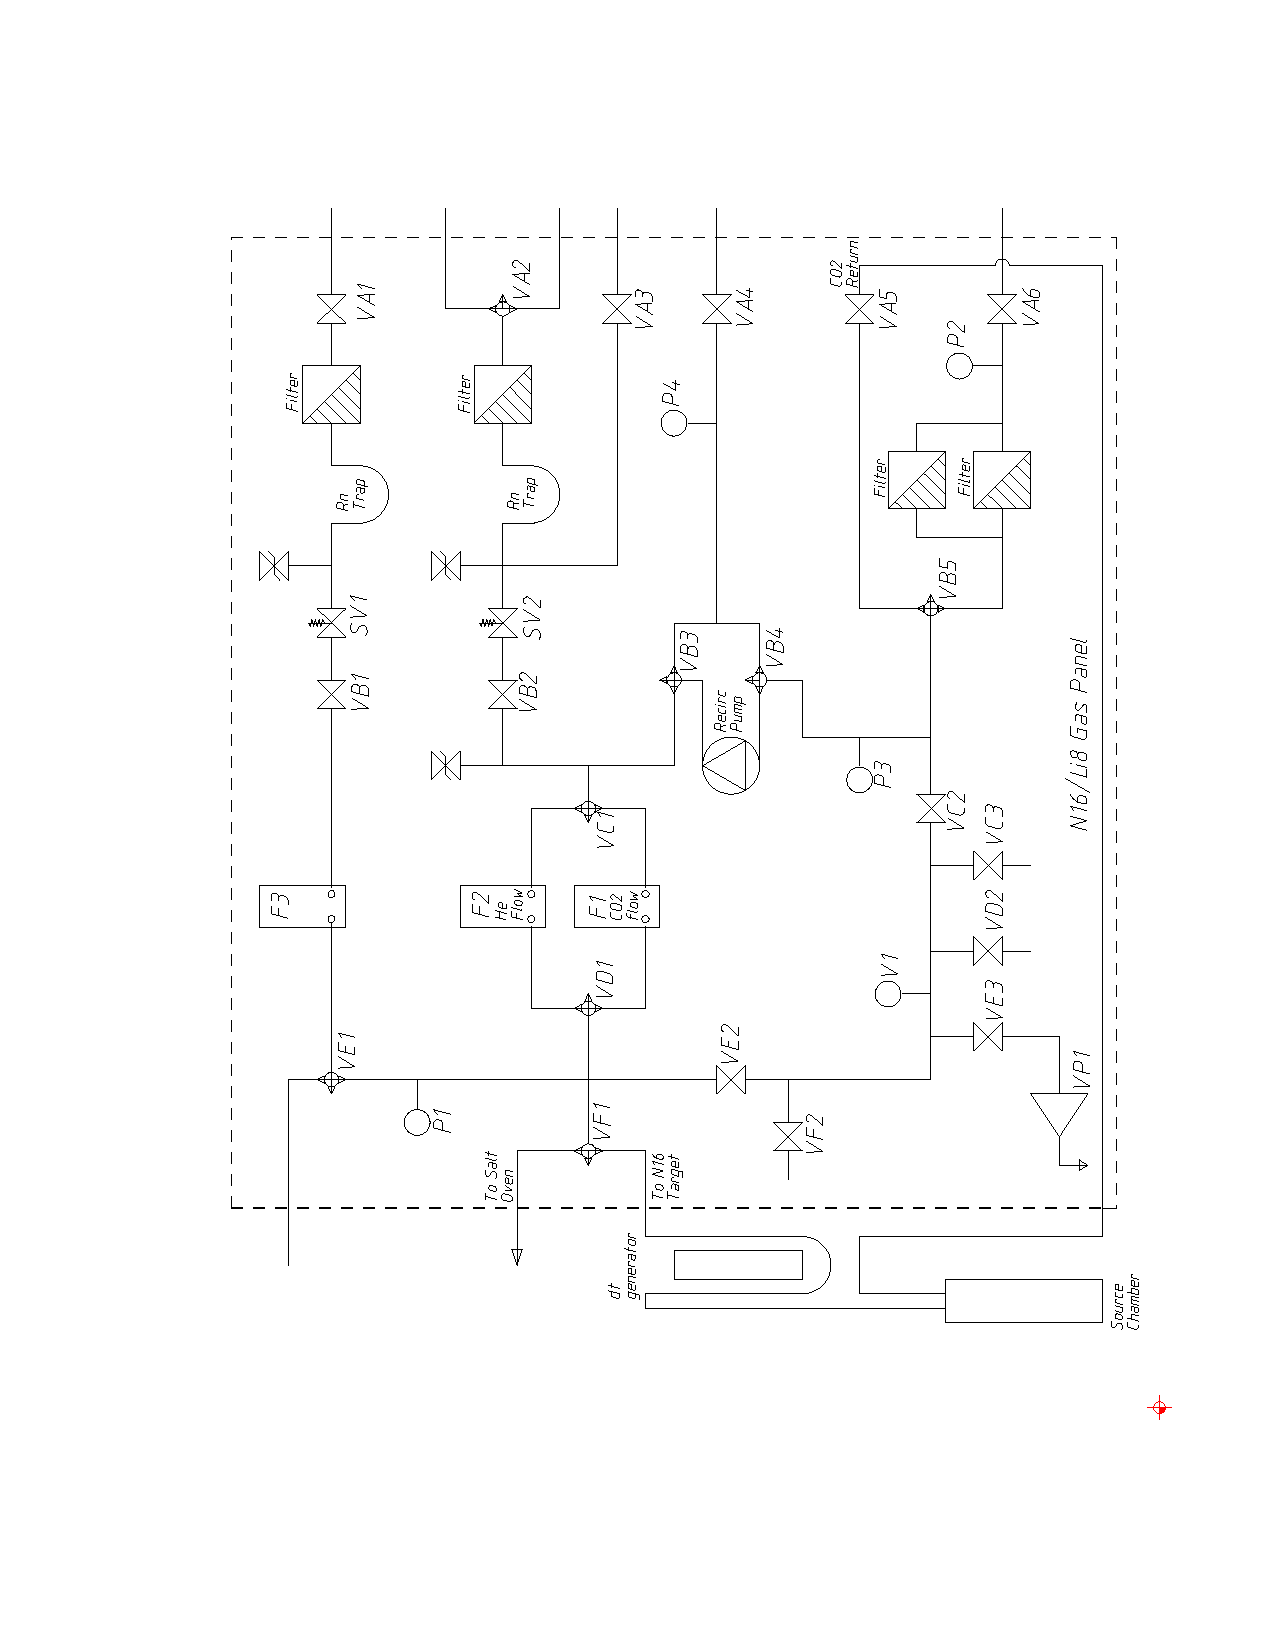
\includegraphics[width=\textwidth]{figures/dtgaspanelschema.pdf}
	\end{center}
	\caption{N16 Gas Panel}
	\label{fig:n16gaspanel}
\end{figure}

\begin{enumerate}
\item \CheckBox[name=gbsp1]{} Verify all valves on the gas board are closed.
\item \CheckBox[name=gbsp2]{} Verify the N$_{2}$/CO$_{2}$ flow control (side B) is off (fully CCW).
\item \CheckBox[name=gbsp3]{} Verify the Solenoid Valve II switch is in the OFF position.
\item \CheckBox[name=gbsp4]{} Enter the DCR using standard entry procedure and verify that
\begin{itemize}
\item \CheckBox[name=gbsp4a]{} the gas input line is connected to the "dry" end of the umbilical
\item \CheckBox[name=gbsp4b]{} the "blue" valve is in the open position
\item \CheckBox[name=gbsp4c]{} the gas return line is connected to the "dry" end of the umbilical 
\item \CheckBox[name=gbsp4d]{} the pressure transducer is powered up and that a voltmeter is connected to it.
\item \CheckBox[name=gbsp4e]{} the voltmeter is reading the correct (18 psi) "pressure".
\end{itemize}
{\it The pressure transducer is hooked up in a temporary way for the time being. Consult the OCE for details.}
\item \CheckBox[name=gbsp5]{} Turn on the power on the main instrument panel and the dual flow controller box.
\item \CheckBox[name=gbsp6]{} Flip the switch on flow controller box to "B" (for N$_{2}$ and/or CO$_{2}$). The reading takes a few minutes to equilibrate to zero or near zero.
\item \CheckBox[name=gbsp7]{} Ensure that the C)$_{2}$ bottle is hooked up to the input line at valve VA2.
\item \CheckBox[name=gbsp8]{} Check that VA2 is closed.
\item \CheckBox[name=gbsp9]{} Close the needle valve on the CO$_2$ bottle.
\item \CheckBox[name=gbsp10]{} Open the main CO$_2$ bottle valve.
\item \CheckBox[name=gbsp11]{} Set the regulator to 80 PSIG. note that once the gas starts flowing the regulator and bottle starts to cool off and you sill have to readjust the setting.
\item \CheckBox[name=gbsp12]{} Record the bottle pressure:
\begin{center}
\begin{tabular}{|c|c|}
\hline
Transducer & Reading \\
\hline
CO$_{2}$ Bottle Pressure & \\
(PSIG) & \\
\hline
\end{tabular}
\end{center}
{\it The pressure of a full bottle is 850 to 900 psi G. The CO$_{2}$ in the bottle is in liquid or solid form and the pressure will stay relatively high until gas only and will drop rapidly thereafter. The CO$_{2}$ regulator has a small white plastic insert (disc with samll hole) in order to seal to the bottle. Don't damage or lose it.}
\item \CheckBox[name=gbsp13]{} Open the inline needle valve after the CO$_2$ regulator.
\item \CheckBox[name=gbsp14]{} Open SVII by setting the switch on the main control panel to {\bf MAN}.
\item \CheckBox[name=gbsp15]{} Open the manual shut-off valve VB2.
\item \CheckBox[name=gbsp16]{} Direct flow to the CO$_2$/N$_2$ flow meter using valve VC1.
\item \CheckBox[name=gbsp17]{} Set the CO$_2$/N$_2$ flow meter to manual and turn the control knob on turn so that some gas will flow.
\item \CheckBox[name=gbsp18]{} Direct flow towards the CO$_2$/N$_2$ flow meter using valve VD1.
\item \CheckBox[name=gbsp19]{} Direct flow to the N16 target chamber using valve VF1. Make sure you are not sending it to the oven!
\item \CheckBox[name=gbsp20]{} Open valve VF2 to accept the returning CO$_2$.
\item \CheckBox[name=gbsp21]{} Open valve VC2.
\item \CheckBox[name=gbsp22]{} Direct the flow towards the exhaust using valve VB4.
\item \CheckBox[name=gbsp23]{} Open the exhast needle valve VA4 fully.
\item \CheckBox[name=gbsp24]{} {\bf Slowly} open valve VA2 and look to see if gas is flowing.
\item \CheckBox[name=gbsp25]{} {\bf Slowly} increase the flow until you reach around a 200-280 reading. Make sure P1 never goes above 100 PSIA. Remember that the time constants are long.
\item \CheckBox[name=gbsp26]{} Record Gas Pressure and Flow.
\begin{center}
\begin{tabular}{|c|c|}
\hline
Transducer & Reading \\
\hline
P1 & \\
(PSIA) & \\
\hline
P2 & \\
(PSIA) & \\
\hline
P3 & \\
(PSIA) & \\
\hline
P4 & \\
(PSIA) & \\
\hline
Flow & \\
(cc/s x (1/1000)) & \\
\hline
Target & \\
Position & \\
\hline
\end{tabular}
\end{center}
\item \CheckBox[name=gbsp27]{} Go back to the DCR and verify that the pressure in the N16 source chamber is within the acceptable upper limit. {\it This is done by checking the voltage reading from the pressure transducer. The transducer gets its power from the monitor PMT supply. Contact the OCE for details.}
\end{enumerate}
\pagebreak

\subsection{ Adjusting the neutron generator target position}

This procedure describes how to change the position of the neutron generator target ladder position. This procedure is used to move from the N16 target to the Li8 target or to adjust the neutron capture efficiency on a target (for example if it is desired to decrease the N16 rate). The nominal target positions for the N16 and Li8 are listed in table \ref{tab:ngenpos}
\begin{table}
\begin{center}
\begin{tabular}{|c|c|}
\hline
Target & Position \\
\hline
N16 & 36.4 \\
Li8 & 101 \\
\hline
\end{tabular}
\caption{Neutron Generator Target Positions}
\end{center}
\label{tab:ngenpos}
\end{table}

{\bf Procedure}

\begin{center}
\begin{tabular}{|c|c|p{7cm}|l|}
\hline
\multicolumn{4}{|l|}{Adjusting Neutron Generator Target Position}\\
\hline
& & & \\
Date & Initial & Procedure & Data and Comments \\
& & & \\
\hline
& & & \\
& & Turn on Power & \\
& & & \\
\hline
& & & \\
& & Run switch in down position & \\
& & & \\
\hline
& & & \\
& & Stop switch in down position & \\
& & & \\
\hline
& & & \\
& & in1 in up position & \\
& & & \\
\hline
& & & \\
& & in2 in up position & \\
& & & \\
\hline
& & & \\
& & in3 in up position & \\
& & & \\
\hline
& & & \\
& & speed set to HIGH & \\
& & & \\
\hline
& & & \\
& & Use jog forward/reverse to change position to desired position & \\
& & & \\
\hline
& & & \\
& & Turn off controller box & \\
& & & \\
\hline
\end{tabular}
\end{center}

\subsection{ N16 PMT turn on procedure}

This procedure describes how to turn on the N16 monitoring PMT.

\begin{enumerate}
\item \CheckBox[name=n16pmt1]{} Verify that the HV controller is turned off and that the dial is turned fully CCW.
\item \CheckBox[name=n16pmt2]{} Verify that the controller cable is plugged into the HV controller.
\item \CheckBox[name=n16pmt3]{} Verify that the controller cable is connected to the "dry" end of the umbilical.
\item \CheckBox[name=n16pmt4]{} Connect a fast oscilloscope to the linear PMT output at the "dry" end of the umbilical. Terminate with a (real) 50 $\Omega$ resistor.
\item \CheckBox[name=n16pmt5]{} Set scope to something link 10 mV per division vertical, 10-20 ns per division horizontal, trigger on negative edge. Use AUTO trigger at first to verify presence of baseline/noise.
\item \CheckBox[name=n16pmt6]{} Turn on the NIM bin.
\item \CheckBox[name=n16pmt7]{} Turn on HV switch.
\item \CheckBox[name=n16pmt8]{} Start dialling (slowly!) up the HV while watching the scope. You should see the glitches and changes in baseline on the scope as you do so. If not stop immediately and check the scope is setup correctly.
\item \CheckBox[name=n16pmt9]{} Real PMT signals should be evident at a voltage setting at of above 2.00.
\item \CheckBox[name=n16pmt10]{} Slowly increase the setting to 2.37 while watching for signs of breakdown. If you see any {\bf stop immediately} and reduce the voltage. Contact the OCE. {\it There may be a tag attached to the power supply with a different voltage than the one listed above. Always use the value on the tag if there is one.}
\item \CheckBox[name=n16pmt11]{} Disconnect the scope.\\ The next steps need only be done if this procedure is executed as part of a general N16 procedure.
\item \CheckBox[name=n16pmt12]{} Verify that the FECD input at 17/15/4
  is disconnected. Leave the ''tee'' and 50 $\Omega$ terminator in place.
\item \CheckBox[name=n16pmt13]{} Use the N16 custom cable to connect the N16 PMT to the correct spigot near the door. Cable tie this cable to the URM. Don't cable tie to the "dry" end part of the N16 cable! \\ {\it It is important that this cable be a short as possible to get the correct trigger timing. Don't just use any random cable you find. Use the correct cable. Also the "dry" end of the N16 PMT cable is fragile. Do {\bf not} cable tie to it. Cable tie to the long cable instead.}
\item \CheckBox[name=n16pmt14]{} Do not connect 17/15/4 until permission has been obtained from the detector operator.
\end{enumerate}

\subsection{ N16 PMT turn off procedure}

This procedure describes how to turn off the N16 monitoring PMT.
\begin{enumerate}
\item \CheckBox[name=n16pof1]{} Disconnect the cable at 17/15/4. Leave
  the "tee" and the 50 $\Omega$ terminator in place.
\item \CheckBox[name=n16pof2]{} Disconnect the cable going from the "dry" end to the patch panel near the door. Coil it up and hang it on the cable rack.
\item \CheckBox[name=n16pof3]{} Turn down (slowly!) the HV control to a dial setting of zero.
\item \CheckBox[name=n16pof4]{} Turn off the HV supply.
\item \CheckBox[name=n16pof5]{} Turn off the NIM bin.\\ {\it This also turns off the power to the pressure transducer. You may have to delay the last two steps until a later time.}
\end{enumerate}

\pagebreak
\subsection{ N16 source startup procedure}

This procedure describes how to turn on the N16 source. An authorized DT and N16 operator is required to perform this procedure.

{\bf State Prior To This Procedure}
\begin{itemize}
\item \CheckBox[name=sspp1]{} DT generator is OFF.
\item \CheckBox[name=sspp2]{} Gas flow to N16 gas board and chamber is OFF.
\item \CheckBox[name=sspp3]{} N16 chamber is assembled and connected to gas board.
\end{itemize}

{\bf Summary of Procedure}
\begin{itemize}
\item \CheckBox[name=sopn161]{} Turn on DT generator.
\item \CheckBox[name=sopn162]{} Set up the N16 gas board.
\item \CheckBox[name=sopn163]{} Turn on the CO$_2$ gas flow to the gas board.
\item \CheckBox[name=sopn164]{} Adjust to desired flow rate.
\item \CheckBox[name=sopn165]{} Check pressure in N16 source chamber.
\item \CheckBox[name=sopn166]{} Turn on N16 PMT.
\item \CheckBox[name=sopn167]{} Adjust NOC and target position to desired $^{16}$N rate.
\end{itemize}

\begin{tabular}{|c|c|}
\hline
\multicolumn{2}{|l|}{}\\
\multicolumn{2}{|l|}{\bf N16 Source Startup Procedure}\\
\multicolumn{2}{|l|}{}\\
\hline
& \\
\TextField[name=dttfop,backgroundcolor=0.975 0.975 0.975,width=2cm]{Operator: } &
\TextField[name=dttfd,backgroundcolor=0.975 0.975 0.975,width=4cm]{Date: } \\
& \\
\hline
\end{tabular}
\begin{itemize}
\item \CheckBox[name=n16p1]{} Complete DT Generator startup procedure.
\item \CheckBox[name=n16p2]{} Complete Gas Board startup procedure.
\item \CheckBox[name=n16p3]{} Complete N16 PMT Turn On procedure.
\item \CheckBox[name=n16p4]{} Complete $^{16}$Detector Setup procedure.
\end{itemize}

\pagebreak
\subsection{ N16 source shutdown procedure}
\begin{tabular}{|c|c|}
\hline
& \\
\TextField[name=dttfop,backgroundcolor=0.975 0.975 0.975,width=2cm]{Operator: } &
\TextField[name=dttfd,backgroundcolor=0.975 0.975 0.975,width=4cm]{Date: } \\
& \\
\hline
\end{tabular}
\begin{enumerate}
\item \CheckBox[name=n16ssp1]{} Close the main CO$_{2}$ gas bottle valve.
\item \CheckBox[name=n16ssp2]{} Wait for pressure on P1, P2, P3, P4 to reach atmosphere (approximately18 PSIA).
\item \CheckBox[name=n16ssp3]{} Turn off regulator on CO$_{2}$ bottle.
\item \CheckBox[name=n16ssp4]{} Close inline valve near CO$_{2}$ regulator.
\item \CheckBox[name=n16ssp5]{} Close VA2.
\item \CheckBox[name=n16ssp6]{} Close SVII by flipping the switch on the main controller panel to {\bf Off}.
\item \CheckBox[name=n16ssp7]{} Close VB2.
\item \CheckBox[name=n16ssp8]{} Close VC1.
\item \CheckBox[name=n16ssp9]{} Turn the flow control knob to zero.
\item \CheckBox[name=n16ssp10]{} Close VD1.
\item \CheckBox[name=n16ssp11]{} Close VF1.
\item \CheckBox[name=n16ssp12]{} Close VF2.
\item \CheckBox[name=n16ssp13]{} Close VC2. 
\item \CheckBox[name=n16ssp14]{} Close VB4.
\item \CheckBox[name=n16ssp15]{} Close VA4.
\item \CheckBox[name=n16ssp16]{} Turn OFF power to Flowmeter, Stepper Motor panel and main instrument panel.
\end{enumerate}

\pagebreak
\subsection{ DT pit disassembly procedure}

This procedure describes how to disassemble the DT pit and how to remove the DT generator. Only qualified and authorised personnel are allowed to do this. Note that his task involves lifting and moving heavy objects. Make sure everyone involved is aware of the potential hazards (pinchpoints etc.) and make sure everyone is aware of what is to happen next. The DT generator and the stand should be treated as if contaminated until properly surveyed --- this means people handling it should be wearing gloves and the gloves should be disposed of in an appropriate manner. 
\begin{enumerate}
\item \CheckBox[name=dtpdp1]{} Ensure that the DT generator is off, the key has been removed and that the AC power to the controller has been disconnected.
\item \CheckBox[name=dtpdp2]{} Ensure that the gas system has been vented and that it is at room pressure.
\item \CheckBox[name=dtpdp3]{} Disconnect control cable from DT generator at electronics module and tag it.
\item \CheckBox[name=dtpdp4]{} Disconnect interlock cables at blocks.
\item \CheckBox[name=dtpdp5]{} Verify that survey meter is working and calibrated.
\item \CheckBox[name=dtpdp6]{} Do a survey of the blocks and surrounding area.
\item \CheckBox[name=dtpdp7]{} Remove top shielding block.
\item \CheckBox[name=dtpdp8]{} Do a survey around the bottom block.
\item \CheckBox[name=dtpdp9]{} Remove bottom block.
\item \CheckBox[name=dtpdp10]{} Survey area.
\item \CheckBox[name=dtpdp11]{} Remove cover over channel. Lift out cables.
\item \CheckBox[name=dtpdp12]{} Back off spacers holding the stand.
\item \CheckBox[name=dtpdp13]{} Lift DT generator stand about 12 inches.
\item \CheckBox[name=dtpdp14]{} Survey.
\item \CheckBox[name=dtpdp15]{} Continue lifting the stand until it cannot go any higher. Do survey every 12-16 inches. Note that the radiation level around the source itself is significantly higher than the rest. Take appropriate precautions.
\item \CheckBox[name=dtpdp16]{} Lift and swing out the bottom of the stand. Watch that the hook does not come off. 
\item \CheckBox[name=dtpdp17]{} Lower the stand to horizontal.
\item \CheckBox[name=dtpdp18]{} Disconnect the FNFM (mark the cables!) and make sure its position is marked relative to the head.
\item \CheckBox[name=dtpdp19]{} Undo the clamps securing the DT generator.
\item \CheckBox[name=dtpdp20]{} Carefully pull out the DT generator.
\item \CheckBox[name=dtpdp21]{} Attach end caps and place in shipping container.
\end{enumerate}

\subsection{ DT pit assembly procedure}

This procedure describes how to install the DT generator and how to assemble the DT pit. Only qualified and authorized personnel are allowed to do this. Note that this task involves lifting and moving heavy ohjects. Make sure everyone involved is aware of the potential hazards (pinchpoints etc.) and make sure everyone is aware of what is to happen next. The DT generator and the stand should be treated as if contaminated until properly surveyed --- this means people handling it should be wearing gloves and the gloves should be disposed of in an appropriate manner.
\begin{enumerate}
\item \CheckBox[name=dtpap1]{} Measure pressure at either end cap to determine if any leaks have developed.
\item \CheckBox[name=dtpap2]{} Remove end caps.
\item \CheckBox[name=dtpap3]{} Slide DT generator into the stand. Be careful not to hit anything.
\item \CheckBox[name=dtpap4]{} Mount clamps securing it. 
\item \CheckBox[name=dtpap5]{} Attach FNFM and connect wires. Make sure signal and HV cables are not interchanged. Ensure FNFM is in correct location.
\item \CheckBox[name=dtpap6]{} Hoist the stand into a vertical position and swing the end into the steel tube.
\item \CheckBox[name=dtpap7]{} Do a sanity check (no cables or gas tubes caught or pinched? No loose parts etc.)
\item \CheckBox[name=dtpap8]{} Lower stand into pit.
\item \CheckBox[name=dtpap9]{} Ensure AC to DT controller is disconnected and the control cable is disconnected from the electronics module.
\item \CheckBox[name=dtpap10]{} Connect the control cable to DT generator. Connect interlock cables.
\item \CheckBox[name=dtpap11]{} Make sure water sensors are in place both inside and outside the stainless steel sleeve. 
\item \CheckBox[name=dtpap12]{} Place cables in channel and position cover over top.
\item \CheckBox[name=dtpap13]{} Lift bottom block into position.
\item \CheckBox[name=dtpap14]{} Lift top block into position
\item \CheckBox[name=dtpap15]{} Connect interlocks.
\item \CheckBox[name=dtpap16]{} Connect control cable to electronics module.
\item \CheckBox[name=dtpap15]{} Connect AC power to controller.
\end{enumerate}

\subsection{ NCD counter calibration procedure}

This procedure describes how to cross-calibrate the NCD counter. It is to be carried out by qualified and authorized persons only.
\begin{enumerate}
\item \CheckBox[name=ncdcc1]{} Turn on the NCD counter and set HV to 1850 V (see DT generator startup procedure).
\item \CheckBox[name=ncdcc2]{} Place $^{252}$Cf source (horizontally) on top of the NCD counter (at the "NCD" label).
\item \CheckBox[name=ncdcc3]{} Recored count rate in log book. {\it the expected count rate in this configuration is 106.2 counts per minute (March 30/2005)}
\item \CheckBox[name=ncdcc4]{} Remove source.
\item \CheckBox[name=ncdcc5]{} Measure background count rate.  {\it Should be $\approx$ 15.5 per minute}
\item \CheckBox[name=ncdcc6]{} Turn on DT generator (see DT generator startup procedure) and record count rate at miniumum and maximum NOC rates. {\it Expected count rates ar 3 and 18 per second at minimum and maximum NOC rates respectively.}
\item \CheckBox[name=ncdcc7]{} Turn off DT generator.
\item \CheckBox[name=ncdcc8]{} Turn off NCD counter.
\end{enumerate}

\section{Revision History}
\begin{tabular}{|c|c|c|p{6cm}|}
\hline\hline
\multicolumn{4}{|l|}{Originating Date: 2017-08-08}\\
\hline
Revision No. & Effective Date & Author & Summary of Change \\
& (YYYY-MM-DD) & & \\
\hline
01 & 2017-08-23 & Ryan Bayes & Drafted from SNO Calibration Operators Manual (PCA, Revision 2) with minor revisions.\\
\hline
02 & 2018-05-30 & Ryan Bayes & Updated with minor corrections and
branding correction\\
\hline
& & & \\
\hline \hline

\end{tabular}




\fancyhf{}
% \lhead{\begin{tabular}{|p{8.25cm}} \hline {\large \bf SNO+ Laser Procedures} \\ \\ \\ \\ \end{tabular}}
\lhead{\begin{tabular}{|p{8.25cm}|p{6cm}|}  
	\hline 
		{\large \bf Salt Oven Usage Procedures}  
										& Document No:  \\ 
								\cline{2-2} & Revision No: 01\\  
								\cline{2-2} & Effective Date: 2018-04-30\\ 
								\cline{2-2} & Page \thepage \\  \end{tabular}}




\begin{tabular}{||l|l|l||}
\hline\hline
& \multicolumn{2}{p{8cm}||}{\bf Salt Oven Usage Procedures} \\

\includegraphics[width=6cm]{figures/SNOplus_logo.png} & \multicolumn{2}{p{8cm}||}{} \\
\hline
\multicolumn{2}{||p{8.5cm}|}{Document Number:} & Revision Number: 01\\
\hline
\multicolumn{3}{||l||}{Document Owner: SNO+ Calibration Post-Doc} \\
\hline
\multicolumn{3}{||l||}{Reviewer:}\\
\hline
Name: & Signature & Date \\
\hline
\multicolumn{3}{||l||}{Authorizer:}\\
\hline
Name: & Signature & Date \\
\hline\hline
\end{tabular}
\thispagestyle{empty}


\section{Purpose}
This document describes the procedure for preparing and operating the Barnstead Thermolyne F21100 for use with a Sodium Chloride (NaCl) loaded quartz tube. The tube furnace heats the salt to a desired temperature of ~610C, just below its melting point. A stream of Helium flows through the heated tube, along with the heated NaCl aerosol. The tube has a water cooling section before the gas outlet, preventing damage to the following gas lines and the Umbilical. 

These procedures are meant to suppliment the use of the DT generator
in the operation of the Cherenkov source for the production of
$^{8}$Li. Any operations that will require the salt oven will also
require the DT Generator procedures. Some operations given here will
supercede those given in the DT Generator procedures as stated in the
Cherenkov deployment procedures. 

\paragraph{Warnings}
\begin{small}
Refer to THA for required precautions needed for tube furnace operations. 
Always use heat resistance gloves when handling the salt tube.
Ensure a proper barricade is in place around the oven work space.
Ensure proper signage is in place to warn others of the hazards present beyond the barricade. 
\end{small}

\section{Procedures}
\subsection{Preparing Oven}
\begin{enumerate}
\item \CheckBox[name=oprep1]{} Only use Tube Furnace in designated area
\item \CheckBox[name=oprep2]{} Make sure the furnace is empty before loading the salt tube
\item \CheckBox[name=oprep3]{} Load the salt tube in the oven
\item \CheckBox[name=oprep4]{} Connect Helium gas inlet and outlet to the tube
\item \CheckBox[name=oprep5]{} Connect the output end to the water cooling loop using the attached flex hose
\end{enumerate}

\subsection{Starting Water Cooling Loop}
\begin{enumerate}
\item \CheckBox[name=cloop1]{} Ensure the needle valve behind the gas board is closed.
\item \CheckBox[name=cloop2]{} Check that the inlet line is attached to the water line after the valve and that the outlet line is running into the drain channel.
\item \CheckBox[name=cloop3]{} Insert the input line into the sleeve on the salt tube closer to the oven. Clamp the line using the hose clamp provided.
\item \CheckBox[name=cloop4]{} Insert the output line into the sleeve on the salt oven nearer to the He gas outlet. Clamp the line using the hose clamp provided.
\item \CheckBox[name=cloop5]{} Slowly open the valve. Ensure that all of the bubbles are out of the line before starting the Helium flow.
\item \CheckBox[name=cloop6]{} Check the seal on the input and output lines for water leaks. If the water pressure is too high water will leak from the cooling loop connections. If there is a leak close the water valve until the leak is no longer present.
\end{enumerate}


\subsection{Turn on Oven}
\begin{enumerate}
\item \CheckBox[name=toov1]{} {Turn on the furnace, make sure the setpoint is 615C}
\item \CheckBox[name=toov2]{} {Use the “UP” or “DOWN” button while in the home display to change the setpoint}
%\end{eu}
\subsubsection{Tuning Cycle}
%\begin{itemize}
\item \CheckBox[name=toov3]{} {Press the “PAGE” button until “Atun” is displayed}
\item \CheckBox[name=toov4]{} {Press the “SCROLL” button, the display will read \textbf{tunE}}
\item \CheckBox[name=toov5]{} {Press either “UP” or “DOWN”  to select \textbf{ON}}
\item \CheckBox[name=toov6]{} {Press both “SCROLL” and “PAGE” to return to the main display }
\item \CheckBox[name=toov7]{} {Wait for the tuning to complete}
%\end{}
\subsubsection{Continuous Heating}
%\begin{itemize}
\item \CheckBox[name=toov8]{} {Press the “PAGE” button until \textbf{SP} is displayed }
\item \CheckBox[name=toov9]{} {Press the “SCROLL” button until \textbf{tm.OP} is displayed }
\item \CheckBox[name=toov10]{} {Press either “UP” or “DOWN”  to select \textbf{Opt.2}. This setting will ramp and maintain setpoint temperature}
\item \CheckBox[name=toov11]{} {Press the “SCROLL” button until \textbf{StAt} is displayed}
\item \CheckBox[name=toov12]{} {Press either “UP” or “DOWN”  to select \textbf{run} }
\item \CheckBox[name=toov13]{} {Press both “SCROLL” and “PAGE” to return to the main display  }
\end{enumerate}

\section{Flow Gas}
\begin{enumerate}
\item \CheckBox[name=gflow1]{} Ensure that all of the valves on the gas board are closed.
\item \CheckBox[name=gflow2]{} Check that the valves on the He, N$_{2}$, and CO$_{2}$ bottles are closed.
\item \CheckBox[name=gflow3]{} Verify that the "Solenoid Valve II" switch is in the OFF position.
\item \CheckBox[name=gflow4]{} Enter the DCR using standard entry procedure and verify that
	\begin{itemize}
	\item \CheckBox[name=gflow5]{} the gas input line is connected to the "dry" end of the umbilical
	\item \CheckBox[name=gflow6]{} the gas return line is connected to the "dry" end of the umbilical.
	% \item the pressure transducer is powered up and that a voltmeter is connected to it
	\end{itemize}
\item \CheckBox[name=gflow7]{} Turn on the power onf the main instrument panel and the dual flow controller box.
\item \CheckBox[name=gflow8]{} Flip the switch on the flow controller box to "B" (for N$_{2}$ and/or CO$_{2}$). The reading takes a few minutes to equilibrate to zero or near zero. 
\item \CheckBox[name=gflow9]{} Ensure that the CO$_{2}$ and He bottles are hooked up to the input line at VA2. Ensure that the N$_{2}$ bottle is connected to VA1.
\item \CheckBox[name=gflow10]{} Check that VA2 and VA2 are closed.
\item \CheckBox[name=gflow11]{} Close the needle valve on the CO$_2$ bottle.
\item \CheckBox[name=gflow12]{} Open the main valves on the CO$_{2}$, He and N$_{2}$ bottles.
\item \CheckBox[name=gflow13]{} Set the regulator on the CO$_{2}$ and He bottle to 33~psi. Set the N$_{2}$ regulator to 20~psi.
\item \CheckBox[name=gflow14]{} Record the bottle pressure:
\begin{center}
\begin{tabular}{|c|c|}
\hline
Transducer & Reading \\
\hline
CO$_{2}$ Bottle Pressure & \\
\hline
He Bottle Pressure & \\
\hline
N$_{2}$ Bottle Pressure & \\
\hline
\end{tabular}
\end{center}
{\emph The pressure of a full CO$_{2}$ bottle is 850 to 900~psi. The
  CO$_{2}$ in the bottle is in liquid or solid form and the pressure
  will stay relatively high until gas only and will drop rapidly
  thereafter. The helium bottle is simply gas under pressure and the
  pressure will drain steadily throughout its use. }
% \item Open the inlie needle valve after the CO$_{2}$ regulator.
\item \CheckBox[name=gflow15]{} Open SVII by setting the switch on the main control panel to
  {\bf MAN}.
\item \CheckBox[name=gflow16]{} Open the manual shut off valve VB2
\item \CheckBox[name=gflow17]{} Direct flow to the He flow meter using valve VD1.
\item \CheckBox[name=gflow18]{} Set the He flow meter to manual and turn the control knob one
  turn so that some gas will flow.
\item \CheckBox[name=gflow19]{} Direct flow towards the He flow meter using valve VD1.
\item Direct flow to the Salt Oven using valve VF1.
\item \CheckBox[name=gflow20]{} Open SVI by setting the switch on the main control panel to
  {\bf MAN}.
\item \CheckBox[name=gflow21]{} Open the manual shut off valve VB1.
\item \CheckBox[name=gflow22]{} Set the N$_{2}$ flow meter to manual and turn the control knob
  one quarter turn.
\item \CheckBox[name=gflow23]{} Direct the N$_{2}$ flow toward P1 (and VF1) so that the N$_{2}$
  mixes with the He flow.
\item \CheckBox[name=gflow24]{} Open valve VF2 to accept the returning CO$_{2}$.
\item \CheckBox[name=gflow25]{} Open valve VC2.
\item \CheckBox[name=gflow26]{} Direct the flow towards the exhaust using valve VB4.
\item \CheckBox[name=gflow27]{} Open the exhast needle valve VA4 fully.
\item \CheckBox[name=gflow28]{} {\bf Slowly} open valve VA2 and look to see if gas is flowing.
\item \CheckBox[name=gflow29]{} {\bf Slowly} increase the flow until you reach around a 200-280
  reading. Make sure P1 never goes above 100 PSI. Remember that the
  time constants are long.
\item \CheckBox[name=gflow30]{} Record gas Pressures and Flow.
\begin{center}
\begin{tabular}{|c|c|}
\hline
Transducer & Reading \\
\hline
P1 & \\
(PSIA) & \\
\hline
P2 & \\
(PSIA) & \\
\hline
P1 & \\
(PSIA) & \\
\hline
P2 & \\
(PSIA) & \\
\hline
Flow & \\
(cc/s $\times$ (1/1000)) & \\
\hline
Target & \\
Position & \\
\end{tabular}
\end{center}
  
\end{enumerate}

\section{Turn off Oven}
\begin{enumerate}
\item \CheckBox[name=ofov1]{} {Press the “PAGE” button until \textbf{SP} is displayed }
\item \CheckBox[name=ofov2]{} {Press the “SCROLL” button until \textbf{StAt} is displayed}
\item \CheckBox[name=ofov3]{} {Press either “UP” or “DOWN”  to select \textbf{off} }
\item \CheckBox[name=ofov4]{} {Press both “SCROLL” and “PAGE” to return to the main display  }
\item \CheckBox[name=ofov5]{} {The oven should start to lose heat, let the salt tube cool to ambient temperature}
\item \CheckBox[name=ofov6]{} {Turn off tube furnace}
\end{enumerate}



\chapter{Pumping and Perging Volumes}
\part{Water Calibration Procedures}
\chapter{Laserball PCA}

\fancyhf{}
% \lhead{\begin{tabular}{|p{8.25cm}} \hline {\large \bf SNO+ Laser Procedures} \\ \\ \\ \\ \end{tabular}}
\lhead{\begin{tabular}{|p{8.25cm}|p{6cm}|}  
	\hline 
		{\large \bf SNO+ Laser Ball PCA Procedures}  
										& Document No:  \\ 
								\cline{2-2} & Revision No: 01\\  
								\cline{2-2} & Effective Date: 2017-06-14\\ 
								\cline{2-2} & Page \thepage \\  \end{tabular}}


\begin{tabular}{||l|l|l||}
\hline\hline
& \multicolumn{2}{p{8cm}||}{\bf SNO+ Laser Ball PCA Procedures} \\

\includegraphics[width=6cm]{figures/SNOplus_logo.png} & \multicolumn{2}{p{8cm}||}{} \\
\hline
\multicolumn{2}{||p{8.5cm}|}{Document Number:} & Revision Number: 01\\
\hline
\multicolumn{3}{||l||}{Document Owner: SNO+ Calibration Post-Doc} \\
\hline
\multicolumn{3}{||l||}{Reviewer:}\\
\hline
Name: & Signature & Date \\
\hline
\multicolumn{3}{||l||}{Authorizer:}\\
\hline
Name: & Signature & Date \\
\hline\hline
\end{tabular}
\thispagestyle{empty}

\section{Purpose}

The calibration of the SNO+ PMTs requires a standardized light source. The standardized light is provided by a dye laser coupled to the laserball which may be deployed into the detector AV. 

\section{Supporting Procedures}

This procedure may be supplemented by documents available from the SNO calibration home page
\url{http://www.sno.phy.queensu.ca/private/calibration/index.html}.
These procedures will be reviewed as necessary.\\

{\bf Online Manipulator Documentation} Contains online manual for all commands and operations with the manip program running on the calibration computer. This is the reference source for commands done from the manip console.\\

{\bf Manipulator User Manual} Contains an overview of the manipulator system and descriptions of sources and some procedures. In particular it describes how to start the manmon program for controlling and monitoring the manipulator.\\

{\bf Manipulator Reference Manual} contains technical information on the manipulator.\\ \\ \\ \\ \\ 

\section{Outline}

The outline of the procedure is:
\begin{enumerate}
\item Prepare the laser and URM for use (turn on N$_{2}$ supply etc).
\item Flush URM2 with N$_{2}$ gas to remove O$_{2}$ and Rn. (if the cover gas system is in place)
\item Calibrate URM2 central rope.
\item Lower source into glovebox.
\item Connect side ropes to source. (if not single axis mode)
\item Deploy source into detector.
\item Take PCA data.
\item Retract source to glovebox.
\item Remove side ropes. (if not single axis mode)
\item Retract source into source tube above gatevalve.
\item Shutdown laser and gas flow to laser and URM.
\end{enumerate} 

\section{Procedures}

\begin{tabular}{|p{8cm}|p{5cm}|}
\hline
&\\
\TextField[name=opd,backgroundcolor=0.975 0.975 0.975,width=4cm]{Operator(s):} &
\TextField[name=opd,backgroundcolor=0.975 0.975 0.975,width=2cm]{Date:} \\
&\\
\hline
\end{tabular}

The procedures in this section are intended to be followed sequentially for the PCA calibration except where it is noted that a following procedure can be skipped. Specifically, if the PCA is to be done in {\it single axis} mode, the side ropes do not need to be attached or detached from the source. 
% Procedures supplementary to the main PCA calibration are found in section 8.3.

\begin{enumerate}
\subsection{Prior to PCA}

\item  \CheckBox[name=prior1]{}  Permission for procedure and confirmation of equipment readiness has been received from Head of Calibration Group or the Site Activities Coordinator. \TextField[name=auth,backgroundcolor=0.975 0.975 0.975,width=3cm]{Record authorizer name}
\item \CheckBox[name=prior2]{} Laserball is mounted in URM2 which is mounted on 10" valve on glovebox.
\item \CheckBox[name=prior3]{} 10" gatevalve is closed and locked.

\subsection{Readying Laser and URM for Operation}

\item \CheckBox[name=rluo1]{} Verify that the LN$_{2}$ dewar in the junction is at least 1/4 full. If not, request that it be swapped out with another dewar. Record liquid level of Dewar, 
\begin{center}
\begin{tabular}{|p{6cm}|}
\hline
\\
\TextField[name=lN2l,backgroundcolor=0.975 0.975 0.975,width=2cm]{LN$_{2}$ Level:} \\
\\
\hline
\end{tabular}
\end{center}
\item \CheckBox[name=rluo2]{} Turn on the N$_{2}$ flow to laser from dewar at junction (marked {\bf Gas Use} on dewar).
\begin{center}
\begin{tabular}{|p{6cm}|}
\hline
\\
\TextField[name=tN2t,backgroundcolor=0.975 0.975 0.975,width=2cm]{Note Time:}\\
\\
\hline
\end{tabular}
\end{center}

\item \CheckBox[name=rluo3]{} Turn on the pressure build valve (marked {\bf Pressure Builder} on dewar). The pressure builder valve opens a controlled leak on the dewar to maintain the 150 psi pressure head. If the valve is not opened, the gas pressure to the laser will eventually drop below the operating level.
\item \CheckBox[name=rluo4]{} Contact the Detector Operator and get permission to enter the DCR. Make sure that the DCR activity bit is set and that the detector operator knows that the laser and URM are being prepared for use. 
\item \CheckBox[name=rluo5]{} Turn on light in DCR following standard procedure. (See Detector Operator Manual).
\item \CheckBox[name=rluo6]{If cover gas present:} Remove the flush return line on the URM. The presence of the buffer line makes it difficult to measure the O$_{2}$ from the URM.
\item \CheckBox[name=rluo7]{If cover gas present:} Check that flush inlet line is connected to URM2. If not connect it. Open the valve on the source tube. It may be necessary to valve off other URMs to get sufficient flow.
\item \CheckBox[name=rluo8]{If cover gas present:} Set up Gas Board in ''bypass mode'' for ''URM flush" only. If you are using the high pressure feed {\bf do not exceed} 10 psi on the regulator. Bypass mode maximizes the flow to the URM.
\item \CheckBox[name=rluo9]{If cover gas present:} Check that the flow meter (located at South-East corner of pipe box) is railed. If not, open needle valve near the flowmeter fully. {\bf Flush should continue until O$_{2}$ reading at the rear of the URM is less than 0.8\%.} This may take up to an hour depending on when the URM was last flushed.
\item \CheckBox[name=rluo10]{} Check that the source clamps are in the OUT position. {\bf Both} knobs have to be in the extreme {\bf OUT} position. {\bf WARNING: If the source is moved with the clamps in the IN position, the source, umbilical, and manipulator may be severely damaged!} The clamps are used to secure the source while the URM is being moved on and off the glovebox.
\item \CheckBox[name=rluo11]{} Check the pressure on the air cylinder for the umbilical takeup mechanism. It should be between 45 and 55 psig. {\bf Do not operate the URM if the pressure is below 40 psig.} If the pressure falls below 10 psig at any point (even momentarily) call the \TextField[name=ocecall,backgroundcolor=0.975 0.975 0.975,width=2cm]{OCE}.
\item \CheckBox[name=rluo12]{} Verify that the 10" gate valve is locked in the closed position. The valve is closed when the handle points towards the pipe box and the slot on the handle stem points AWAY from the source tube.
\item \CheckBox[name=rluo13]{} Calibrate the central rope length (see procedure: Central Rope Position Calibration). Record changes in length of central rope and umbilical. 
\begin{center}
\begin{tabular}{|lp{4cm}|}
\hline
 & \\
$\Delta l$ rope & \TextField[name=dlr,backgroundcolor=0.975 0.975 0.975,width=4cm]{}\\
& \\
$\Delta l$ umbilical & \TextField[name=dlu,backgroundcolor=0.975 0.975 0.975,width=4cm]{}\\
& \\
\hline
\end{tabular}
\end{center}
The current fiducial mark for URM2 on the 10" gate valve is $z_{mark} = 1549.3$. Note the fiducial mark is written on the source tube. 
\item \CheckBox[name=rluo14]{} Check that all seals are in place on URM. Including:
	\begin{itemize}
	\item \CheckBox[name=urms1]{} flush inlet line
	\item \CheckBox[name=urms2]{} window on front of URM motorbox
	\item \CheckBox[name=urms3]{} window on rear of URM motorbox
	\item \CheckBox[name=urms4]{} umbilical feedthrough on rear of motorbox
	\item \CheckBox[name=urms5]{} view port window cover on source tube
	\item \CheckBox[name=urms6]{} window on rear of stretcher box
	\end{itemize}
\item \CheckBox[name=rluo15]{} Check that you are familiar with the section on operating the laser especially the {\bf Emergency Shutdown Procedure}. Also, be aware that UV absorbing safety glasses {\bf MUST} be worn while the laser is running unless {\bf ALL} covers on the laser are in place.
\item \CheckBox[name=rluo16]{} Plug in the powercord to the laser.
\item \CheckBox[name=rluo17]{} Check the POWER switch on the laser is to {\bf remote}.
\item \CheckBox[name=rluo18]{} Check the CONTROL switch on the laser is set to {\bf remote}.
\item \CheckBox[name=rluo19]{} Check that the manual shutoff valve on the right of MV5 is open.
\item \CheckBox[name=rluo20]{} Check that the manual shutoff valve MV9 is open.
\item \CheckBox[name=rluo21]{} Reset the "Kill Switch" by pushing the red reset button.
\item \CheckBox[name=rluo22]{} Type \verb+n2laser poweron+ on the manip computer. This turns on the low voltage power and energizes the N$_{2}$ gas valve.
\item \CheckBox[name=rluo23]{} Verify that N$_{2}$ is flowing through flow gauge FG5 to the laser head. If there is no flow consult an expert. {\bf Running the laser without sufficient N$_{2}$ flow causes serious damage to the laser head!}
\item \CheckBox[name=rluo24]{} Record observed laser gas pressure and flow values. Note that the expected values listed below may be superseded by ones listed on one or more tags attached to the valves or flow meters. Always use the values found on the tags.
\begin{center}
\begin{tabular}{|l|c|c|}
\hline
Transducer & Expect & Observed \\
\hline
&&\\
PG2 & 110-150 psig & \TextField[name=pg2,backgroundcolor=0.975 0.975 0.975,width=2cm]{}\\
&&\\
\hline
&&\\
PG3 & 90-110 psig & \TextField[name=pg3,backgroundcolor=0.975 0.975 0.975,width=2cm]{} \\
&&\\
\hline
&&\\
PT4 & 100-110 psig & \TextField[name=pt4,backgroundcolor=0.975 0.975 0.975,width=2cm]{} \\
&&\\
\hline
&&\\
FG5 & $\approx 50$ (bottom of ball) & \TextField[name=fg5,backgroundcolor=0.975 0.975 0.975,width=2cm]{} \\
&&\\
\hline
&&\\
PT6 & $\approx 90$ psig & \TextField[name=pg3,backgroundcolor=0.975 0.975 0.975,width=2cm]{} \\
&&\\
\hline
\end{tabular}
\end{center}
PG2, PG3, and FG5 are read off the gas panel on the end of the laser cabinet. PT4 and PT6 are read from the manipulator computer either from the \verb+manmon+ laser window or using the commands,
\begin{center}
\begin{tabular}{ll}
\verb+n2laser hipressure+ & (for PT4) \\
\verb+n2laser lowpressure+ & (for PT6) \\
\end{tabular}
\end{center}
Gas must flow through the laser for $\approx 10$ min before turning the laser high voltage on.
\item \CheckBox[name=rluo25]{} Block the laser light using the command \verb+n2laser block+.
\item \CheckBox[name=rluo26]{} Select dyecell 4 (500 nm) by typing \verb+dyelaser cell 4+
\item \CheckBox[name=rluo27]{} Check the state of the laser by issuing the command \verb+n2laser monitor+. It will tell you the general state of the laser. 
	\begin{itemize}
	\item \CheckBox[name=lst1]{} Check that all 4 stirmotors are on.
	\item \CheckBox[name=lst2]{} Check that there is 120V to the laser.
	\item \CheckBox[name=lst3]{} Check that the filterwheels do not report any problems.
	\end{itemize}
\item \CheckBox[name=rluo28]{If cover gas present} Wait until the O$_2$ level in the URM is at or below 0.8\%.
\subsection{Deploying Source from Source Tube Into Glovebox}
\item \CheckBox[name=rluo29]{If cover gas present:} Verify that the URM is below 0.8\% O$_{2}$
\item \CheckBox[name=rluo30]{If cover gas present:} Check that flush return line is connected to URM2. If not, connect it. It may be necessary to move it from another URM.
\item \CheckBox[name=rluo31]{} Turn off DCR lights.
\item \CheckBox[name=rluo32]{If cover gas present:} Record the Cover Gas O$_{2}$ level.
\begin{center}
\begin{tabular}{|c|}
\hline
\\
\TextField[name=CGO2,backgroundcolor=0.975 0.975 0.975,width=2cm]{Cover Gas O$_{2}$ Reading:}\\
\\
\hline
\end{tabular}
\end{center}
\item \CheckBox[name=rluo33]{} Establish communications with the detector operator and request that the detector be put in a {\bf Maintenance} run. 
\item \CheckBox[name=rluo34]{} Open gate valve ({\bf Slowly!}). Record the time the valve is opened.
\begin{center}
\begin{tabular}{|c|}
\hline
\\
\TextField[name=tgvo,backgroundcolor=0.975 0.975 0.975,width=2cm]{Time Gate Valve Opened:}\\
\\
\hline
\end{tabular}
\end{center}
\item \CheckBox[name=rluo35]{} Lock gate valve open.
\item \CheckBox[name=rluo36]{} With flashlight perform light leak check on URM. In particular check the seal of the source tube window and around the base of the source tube. Also, check around any inspection panel which may have been removed in the recent past.
\item \CheckBox[name=rluo37]{} Using the dimmer switch, {\bf slowly} bring up breaker 9 lights in the DCR with a person still watching the OWL monitor.
% \item \CheckBox[name=rluo38]{} In ORCA, source type is set to {\bf LASERBALL}.
\item \CheckBox[name=rluo39]{} ORCA is in a {\bf transitional run}.
\item \CheckBox[name=rluo40]{} Verify that {\bf manip\_logger} on the calibration computer and logging the {\bf Laserball} source. Check that it is writing to the database by locating \url{couch.ug.snopl.us/manip/_all_docs} and verify that entries exist for \verb+N2LASER+ and \verb+LASERBALL+ corresponding to the current date.
\item \CheckBox[name=rluo41]{} Check movement of laserball down
\begin{center}
\begin{tabular}{|l|l|}
\hline
console & \verb+ manip > laserball by 0 0 -5+ \\
\hline
manmon & in laserball window: \\ &  set x=0, y=0, z=-5 \\ & click on {\bf move by} \\
\hline
\end{tabular}
\end{center}
The laserball should move down by 5 cm. The tension on the rope should be 40-60 N. The tension on the umbilical should be 10-30 N.
\item \CheckBox[name=rluo42]{} Check that the source offset and orientation is set correctly. At the console type \verb+laserball sourceoffset+. The current laserball has an offset of -64.5 cm. If the reported number is different contact the OCE. FOr single axis deployment mode the orientation should be 0; i.e. confirm from the console by typing \verb+laserball orientation+. It should return \verb+0+. If deployed with side ropes the orientation depends on what direction the slot faces. If in doubt contact the OCE.
\item \CheckBox[name=rluo43]{} Deploy source into the glovebox:
\begin{center}
\begin{tabular}{|l|l|}
\hline
console & \verb+ manip > laserball to 0 0 1380+ \\
\hline
manmon & in laserball window: \\ &  set x=0, y=0, z=1380 \\ & click on {\bf move to} \\
\hline
\end{tabular}
\end{center}

\subsection{Deploying Manipulator into Centre of Detector from Glovebox}
\item \CheckBox[name=rluo44]{} Contact Water Supervisor and advise him/her that the source is being lowered into the AV. The water group maintains a very small differential pressure between the AV water and the cavity water. The volume of the source is enough to disrupt this differential pressure.
\item \CheckBox[name=rlup45]{} Check tensions on urm2rope and urm2umbilical. Rope tension should be appreoximately 30-50 N. Umbilical tension should be between 15-40 N. Note that the tensions are reduced once the sources is submerged.
\item \CheckBox[name=rlup46]{} Move laserball to centre of detector.
\begin{center}
\begin{tabular}{|l|l|}
\hline
console & \verb+ manip > laserball to 0 0 64.5+ \\
\hline
manmon & in laserball window: \\ &  set x=0, y=0, z=64.5 \\ & click on {\bf move to} \\
\hline
\end{tabular}
\end{center}
\subsection{Turning on the Laser}
\item \CheckBox[name=rlup47]{} Verify on the console that the control power on the laser is on: \\ \verb+n2laser monitor+\\ All voltages should be on, all stir motors should be ON, both filterwheels should be IDLE, the dye cell motor should be IDLE and gas should be flowing. If not contact OCE.
\item \CheckBox[name=rlup48]{} Verify that the N2 gas has been flowing through the laser for $\approx 10$~min. Note that the gas flow is turned on and off with the \verb+n2laser poweron/poweroff+ commands.
\item \CheckBox[name=rlup49]{} Select desired wavelength or dye cell
\begin{center}
\begin{tabular}{|l|l|}
\hline
console & \verb+ manip > dyelaser cell <0-9>+ \\
 & or \\
 & \verb+ manip > dyelaser wavelength <wavelength>+ \\
\hline
manmon & in laser window: \\ & click on button above desired dye cell \\
\hline
\end{tabular}
\end{center}
\item \CheckBox[name=rlup50]{} Set ND=6.0 or higher.
\begin{center}
\begin{tabular}{|l|l|}
\hline
console & \verb+ manip > n2laser setnd 6.0+ \\
\hline
manmon & in laser window: $\to$ Windows $\to$ Neutral Density Settings\\
& click on desired neutral density \\
\hline
\end{tabular}
\end{center}
The filter wheels are set to a large attenuation when first turning on the laser to prevent a large amount of light being introduced into the detector and overwhelming the data acquisition. Once the laser is on, the rate and intensity can be adjusted to the desired level.
\item  \CheckBox[name=rlup51]{} Wait for the laser to return status READY
\item  \CheckBox[name=rlup52]{} Turn on the laser light
\begin{center}
\begin{tabular}{|l|l|}
\hline
console & \verb+ manip > n2laser start+ \\
\hline
manmon & in laser window: \\
& click on {\bf light on} \\
\hline
\end{tabular}
\end{center}
Now wait 90 seconds while the trigger is delayed. Laser will come on at 10 Hz trigger rate.
\item  \CheckBox[name=rlup52]{} Plug the Laserball Trigger signal into the EXTA input on the MTCD.
The trigger should be setup from previous PCAs, but the setup should
be verified.
\begin{itemize}
\item \CheckBox[name=vlts1]{} The cable running from port on the dye
laser marked as ``Trigger'' leads to the NIM bin discriminator input.
Ensure that the NIM bin is on.
\item \CheckBox[name=vlts2]{} There should be a jumper across the
``Delay'' channels of the NIM discriminator.
\item \CheckBox[name=vlts3]{} The output channel on the NIM
discriminator should be connected to the ``Input'' channel of the
Stanford Research Pulse Generator. Ensure that the Stanford pulser is
on and is using a trigger delay of 370 ns (press the ``DELAY'' button
to check).
\item \CheckBox[name=vlts4]{} The BNC cable leading to the MTCD should
be connected to the ``A$\sqcap$B'' to make an ECA high signal.
\textbf{Warning: TELLIE also uses the EXTA input. The TELLIE cable
should be placed in a visible location after it is removed from the
MTCD and muts be replaced when the PCA is complete.}
\end{itemize}
\subsection{Taking PCA Data}
\item {\bf PCA Runs} The exact nature of the PCA runs will vary. The "canonical" run tends to be 
	\begin{enumerate}
	\item \CheckBox[name=PCA1]{} Long Low Occupancy Run.
		\begin{itemize}
		\item 500~nm
		\item The centroid for the raw TAC is usually at 1800.
		\item 5-8\% occupancy (ND setting at 500~nm is
	approximately 1.2 to produce less than 500 NHIT per pulse).
		\item 35 Hz laser trigger rate.
		\item Run Type: LASERBALL\_PCA
		\item 10 subruns (2-3 hours)
		\end{itemize}
	\item \CheckBox[name=PCA2]{} Short Medium Occupancy Run.
		\begin{itemize}
		\item 500~nm
		\item The centroid for the raw TAC is usually at 1800.
		\item 20-25\% occupancy (ND setting at 500~nm is approximately 3.0).
		\item 5-10 Hz laser trigger rate (or best you can do without buffer overflow).
		\item Run Type: LASERBALL\_PCA
		\item 3 subruns (20 minjutes).
		\end{itemize}
	\end{enumerate}
	The laser can be run up to 45~Hz but the DAQ produces strange results at such rates.
\subsection{Turning Off Laser}
\item \CheckBox[name=TOL1]{} Unplug EXTA at the MTCD. Replace the
	TELLIE cable.
\item \CheckBox[name=TOL2]{} Turn off laser light  
\begin{center}
\begin{tabular}{|l|l|}
\hline
console & \verb+ manip > n2laser stop+ \\
\hline
manmon & in laser window: \\
& click on {\bf light off} \\
\hline
\end{tabular}
\end{center}
\item \CheckBox[name=TOL3]{} Turn off laser power
\begin{center}
\begin{tabular}{|l|l|}
\hline
console & \verb+ manip > n2laser poweroff+ \\
\hline
manmon & in laser window: \\
& click on {\bf power off} \\
\hline
\end{tabular}
\end{center}
\item \CheckBox[name=TOL4]{} Unplug laser power cord from wall outlet
The laser is unplugged when it is not intended to be used for extended periods. This is because it has been observed that on several occasions after an unscheduled power outage the laser has come up in a funny state.

\subsection{Retracting Manipulator to Glovebox}
\item \CheckBox[name=rmg1]{} Contact Water Supervisor. Inform him/her that the source is about to be removed from the detector.
\item \CheckBox[name=rmg2]{} Retract the laserball from AV into glovebox
 \begin{center}
\begin{tabular}{|l|l|}
\hline
console & \verb+ manip > laserball to 0 0 1300+ \\
\hline
manmon & in laserball window: \\ &  in laserball window:\\ & click on {\bf Position the pivot} \\ & set x=0, y=0, z=1300 \\ & click on {\bf move to} \\
\hline
\end{tabular}
\end{center}
\item \CheckBox[name=rmg2]{} Retract the laserball to position to disconnect side ropes
 \begin{center}
\begin{tabular}{|l|l|}
\hline
console & \verb+ manip > laserball to 0 0 1380+ \\
\hline
manmon & in laserball window: \\ &  in laserball window:\\ & click on {\bf Position the pivot} \\ & set x=0, y=0, z=1380 \\ & click on {\bf move to} \\
\hline
\end{tabular}
\end{center}
When moving the laserball to 1380, it is important to make sure you are moving with respect to the {\bf pivot} and {\bf not} the centre of the source which is 64.5 cm below the pivot. This is especially important if the sideropes are attached!

\subsection{Retracting source above gate valve; Side ropes not attached}
\item \CheckBox[name=sna1]{} Move laserball to 1530
\begin{center}
\begin{tabular}{|l|l|}
\hline
console & \verb+ manip > laserball to 0 0 1530+ \\
\hline
\end{tabular}
\end{center}
\item \CheckBox[name=sna2]{} Move laserball to 1540
\begin{center}
\begin{tabular}{|l|l|}
\hline
console & \verb+ manip > laserball to 0 0 1540+ \\
\hline
\end{tabular}
\end{center}
\item \CheckBox[name=sna3]{} Move laserball to 1550
\begin{center}
\begin{tabular}{|l|l|}
\hline
console & \verb+ manip > laserball to 0 0 1550+ \\
\hline
\end{tabular}
\end{center}
{\bf NOTE:\\
MINIMUM SAFE HEIGHT TO CLOSE GATEVALVE IS 1535~cm\\
If unable to get above this height, contact expert.}
\item \CheckBox[name=sna4]{} Retrieve the gatevalve key from the DCR lock box.
\item \CheckBox[name=sna5]{} Unlock the gatevalve.
\item \CheckBox[name=sna6]{} Carefully close the gate valve by rotating the handle {\it clockwise}. {\it Expect resistance when the handle is about 3.4 of the way to the closed position. This is the normal overcentering of the valve mechanism.} {\bf If resistance is felt before this or if any sounds are heard that might be caused by valve hitting the source, STOP and contact and expert.} Record the time the valve is closed.
\begin{center}
\begin{tabular}{|c|}
\hline
\\
\TextField[name=tgvc,backgroundcolor=0.975 0.975 0.975,width=2cm]{Time Gate Valve Closed:}\\
\\
\hline
\end{tabular}
\end{center}
\item \CheckBox[name=sna7]{} Lock the gatevalve in the {\bf CLOSED} position.
\item \CheckBox[name=sna8]{} Return the gatevalve key to the DCR lock box.
\item \CheckBox[name=sna9]{If cover gas present} Record the Cover Gas O$_{2}$ level
\begin{center}
\begin{tabular}{|c|}
\hline
\\
\TextField[name=cgor,backgroundcolor=0.975 0.975 0.975,width=2cm]{Cover Gas O$_{2}$ Reading:}\\
\\
\hline
\end{tabular}
\end{center}
\item \CheckBox[name=sna10]{If cover gas present} Close the URM flush valve is the source does not need dryiing out. {\it It is desirable to leave a minute flow of N$_{2}$ through the URM in order to dry out the source and the umbilical. Contact OCE for instructions.}
\item \CheckBox[name=sna11]{If cover gas present} Turn off the URM flush regulator (if the source does not need drying out).
\item \CheckBox[name=sna12]{} IF the laser is off, turn off gas flow at the LN$_{2}$ dewar in the junction:
\subsection{After Calibration}
\item \CheckBox[name=ac1]{} Source is above the gate valve.
\item \CheckBox[name=ac2]{} Gate valve is closed and locked.
\item \CheckBox[name=ac3]{} Laser is off.
\item \CheckBox[name=ac4]{} Manual shutoff valve to the right of MV5 is closed.
\item \CheckBox[name=ac5]{} Laser power cord is unplugged from wall outlet.
\item \CheckBox[name=ac6]{} High pressure LN$_{2}$ dewar is turned off (both {\bf Gas Use} valve and {\bf Pressure Building} valve).
\item \CheckBox[name=ac7]{} Flush return line is disconnected from rear of URM2.
\item \CheckBox[name=ac8]{} Gas board is set up to provide sufficient flow to dry out the inside of the URM.
\end{enumerate}

\section{Revision History}
\begin{tabular}{|c|c|c|p{6cm}|}
\hline\hline
\multicolumn{4}{|l|}{Originating Date: 2017-06-14}\\
\hline
Revision No. & Effective Date & Author & Summary of Change \\
& (YYYY-MM-DD) & & \\
\hline
01 & 2017-06-14 & Ryan Bayes & Drafted from SNO Calibration Operators Manual (PCA, Revision 2) with minor revisions and editable blocks added for user notes.\\
\hline
& & & \\
\hline
& & & \\
\hline \hline

\end{tabular}




\chapter{N16 Calibration}

\fancyhf{}
% \lhead{\begin{tabular}{|p{8.25cm}} \hline {\large \bf SNO+ Laser Procedures} \\ \\ \\ \\ \end{tabular}}
\lhead{\begin{tabular}{|p{8.25cm}|p{6cm}|}  
	\hline 
		{\large \bf SNO+ N16 Calibration Procedure}  
										& Document No:  \\ 
								\cline{2-2} & Revision No: 01\\  
								\cline{2-2} & Effective Date: 2017-08-25\\ 
								\cline{2-2} & Page \thepage \\  \end{tabular}}



\begin{tabular}{||l|l|l||}
\hline\hline
& \multicolumn{2}{p{8cm}||}{\bf SNO+ N16 Calibration Procedure} \\

\includegraphics[width=6cm]{figures/SNOplus_logo.png} & \multicolumn{2}{p{8cm}||}{} \\
\hline
\multicolumn{2}{||p{8.5cm}|}{Document Number:} & Revision Number: 01\\
\hline
\multicolumn{3}{||l||}{Document Owner: SNO+ Calibration Post-Doc} \\
\hline
\multicolumn{3}{||l||}{Reviewer:}\\
\hline
Name: & Signature & Date \\
\hline
\multicolumn{3}{||l||}{Authorizer:}\\
\hline
Name: & Signature & Date \\
\hline\hline
\end{tabular}

\thispagestyle{empty}

\section{Purpose}

This procedure describes, step by step, the process of performing an N16 calibration at the centre of the detector in single axis mode. It is intended as a guideline for operators who have been trained on the manipulator and N16. It assumes that the N16 source is mounted on URM3, located on the 6" gatevalve on the UI which is located on the northeast corner.

\section{Outline of the procedure}

\begin{enumerate}
\item Prepare the URM for use (turn on N$_{2}$ supply etc.)
\item Flush URM3 with N$_{2}$ gas to remove room air and radon.
\item Calibrate URM3 central rope.
\item Lower source into UI.
\item Deploy source into detector.
\item Take N16 data.
\item Retract source into source tube above gatevalve.
\item Shutdown N16 gas board and gas flow to laser and URM.
\end{enumerate}
You will need the following procedures to complete an N16 calibration.
\begin{itemize}
\item {\bf N16 Calibration} (this procedure)\\ \\ \\ \\ \\
\item {\bf Central Rope Calibration Procedure} 
\item {\bf DT Generator Turn On Procedure} 
\item {\bf N16 Source Startup Procedure}
\item {\bf N16 Source Shutdown Procedure}
\item {\bf DT Generator Turn Off Procedure}
\end{itemize}

\section{Procedure}

\begin{tabular}{|l|l|}
\hline
\multicolumn{2}{|l|}{} \\
\multicolumn{2}{|l|}{\bf N16 Calibration Procedure} \\
\multicolumn{2}{|l|}{} \\
\hline
& \\
\TextField[name=n16op,backgroundcolor=0.975 0.975 0.975,width=2cm]{Operator: } &
\TextField[name=n16d,backgroundcolor=0.975 0.975 0.975,width=4cm]{Date: } \\
& \\
\hline
\end{tabular}

The procedures in this section are intended to be followed sequentially for the N16 calibration except where it is noted that a following step can be skipped. Specifically, if the N16 is to be done in {\it single axis} mode, the side ropes do not need to be attached or detached from the source.

{\bf Prior to N16}

\begin{enumerate}
\item \CheckBox[name=n16p1]{} Permission for procedure and confirmation of equipment readiness has been received from the Head of the Calibration Group.
\item \CheckBox[name=n16p2]{} N16 is mounted on URM3 which is mounted on the UI 6" gatevalve.
\item \CheckBox[name=n16p3]{} The gatevalve is closed and locked (or the handle is removed).

{\bf Readying N16 Source and URM for Operation}

\item \CheckBox[name=n16p4]{} Contact Detector Operator and verify that the DCR activity bit is set.
\item \CheckBox[name=n16p5]{} Turn on lights in DCR following standard procedure.
\item \CheckBox[name=n16p6]{} Verify that the high pressure N$_{2}$ to the laser is valved off (end of laser, upper right hand corner). 
\item \CheckBox[name=n16p7]{} Verify that all valve on the gas board are closed and the regulator is set to zero.
\item \CheckBox[name=n16p8]{} Remove the flush return line on the URM. {\it The presence of the buffer line makes it difficult to measure the O$_{2}$ from the URM.}
\item \CheckBox[name=n16p9]{} Check that the flush inlet line is connected to URM3. If not connect it. Open the valve at the source tube. {\it It may be necessary to valve off the other URMs to get sufficient flow.}
\item \CheckBox[name=n16p10]{} Verify that the LN$_{2}$ dewar in the junction is at least 1/4 full. If not swap it out with another dewar. Record liquid level of dewar,
\begin{center}
\begin{tabular}{|c|}
\hline
\\
\TextField[name=n16n2l,backgroundcolor=0.975 0.975 0.975,width=2cm]{LN$_{2}$ Level:} \\
\\
\hline
\end{tabular}
\end{center}
\item \CheckBox[name=n16p11]{} Verify that the dewar gas pressure is above 20 psig. If not, swap it out with another dewar. Unlike the laser the $^16$N does not require a minimum of 100 psig N$_{2}$ is only used for flushing. Note that this dewar won't last long if the pressure is below 100 psig.
\item \CheckBox[name=n16p12]{} Turn on the high pressure N$_{2}$ flow from the dewar at junction (Marked {\bf Gas Use} on dewar).
\begin{center}
\begin{tabular}{|c|}
\hline
\\
\TextField[name=n16n2t,backgroundcolor=0.975 0.975 0.975,width=2cm]{Note Time:} \\
\\
\hline
\end{tabular}
\end{center}
\item \CheckBox[name=n16p13]{} Turn on pressure builder valve (Marked {\bf Pressure Builder} on dewar). {\it The pressure builder valve opens a controlled leak on the dewar to maintain the 150 psig pressure head. If the valve is not opened, the gas pressure to the laser and URM will eventually drop below the operating level (10 psig).}
\item \CheckBox[name=n16p14]{} Set up Gas Board in "bypass mode" for "URM flush" only. If you are using the high pressure feed {\bf do not exceed} 10 psi on the regulator. {\it Bypass mod maximizes the flow to the URM. (Gas enters at top left hand corner, flows through the regulator along the outside right hand side line down the URM with all other valves closed --- see the Gas Board Section for details)}.
\item \CheckBox[name=n16p15]{} Check that the flow meter (located at the east side of the pipe box) is railed. If not, open the needle valve near the flowmeter fully.\\ {\bf Flush should continue until O$_{2}$ reading at the rear of the URM is less than 0.8\%.} {\it This may take up to an hour depending on when the URM was last flushed.}
\item \CheckBox[name=n16p16]{} Once the URM is flushedd the N$_{2}$ supply may be switched from the high pressure dewar to the Wessington dewar. Check with the Operations Group first before switching. Do not use the Wessington if a transfer is in progress. Consult the gasboard section for details on how to switch. If the flush is continued from the high pressure deewar reduce the flow using the needle valve. A setting of 2 full turns above the point where the flowmeter rails is sufficient.
\item \CheckBox[name=n16p17]{} Verify (blue) valve on the N16 Umbilical gas feed line (the translucent line is OPEN. If not, open it.
\item \CheckBox[name=n16p18]{} Execute the N16 PMT Turn On Procedure.
\item \CheckBox[name=n16p19]{} Do not connect the PMT trigger cable to channel 4, slot 15 crate 17 before obtaining permission from the detector operator.
\item \CheckBox[name=n16p20]{} Check that the source clamps are in the RELEASE position. There are two clamps. Check both. {\bf WARNING: The clamp positions RELEASE and HOLD are 90 deg apart. Rotate the clamp in the SHORT direction (90 deg) from the HOLD to RELEASE position. The clamp must not be rotated the other way!}\\ {\it The clamps are used to secure the source while the URM is being moved on and off the UI. If the source is moved with the clampes in the HOLD position, it may severely damage the manupulator and the umbilical.}
\item \CheckBox[name=n16p21]{} Check the pressure on the air cylinder for the umbilical takeup mechanism. It should be between around 55 psig. {\bf Do not operate the URM if the pressure is below 40 psig.} If the pressure falls below 10 psig at any point (even momentarily) call the OCE. An internal inspection of the URM is mandatory before operating the unit again. {\it The pressure cylinder on the URM maintains tension on the umbilical takeup reel. A low gas pressure can result in the umbilical falling off the takeup reel and getting caught or jammed leading to destruction of the umbilical.} 
\item \CheckBox[name=n16p22]{} Verify that Gate Valve 3 is closed and locked (or handle is removed). {\it The valve is CLOSED when the handle points towards the pipebox and the slot on the handle stem points AWAY from the source tube.} % Note this will change with the new gate valves
\item \CheckBox[name=n16p23]{} Calibrate Central Rope Length (see procedure {\it Central Rope Position Calibration}). Record changes in length of central rope and umbilical. The current fiducial mark for URM3 on gatevate 3 is 
\[
z_{mark} = 1558.5
\]
Note: the fiducial mark is written on the source tube. If it differs from the above number use what is written on the source tube.
\begin{center}
\begin{tabular}{|c|}
\hline
\\
\TextField[name=n16dl,backgroundcolor=0.975 0.975 0.975,width=3cm]{$\Delta l$ rope:}\\
\\
\hline
\\
\TextField[name=n16du,backgroundcolor=0.975 0.975 0.975,width=2cm]{$\Delta l$ umbilical:}\\
\\
\hline
\end{tabular}
\end{center}
\item \CheckBox[name=n16p24]{} Check that all seals are in place on the URM. Including:
	\begin{itemize}
	\item \CheckBox[name=n16p24a]{} flush inlet line
	\item \CheckBox[name=n16p24b]{} window on front of URM motorbox
	\item \CheckBox[name=n16p24c]{} window on rear of URM motorbox
	\item \CheckBox[name=n16p24d]{} umbilical feedthrough on rear of motorbox
	\item \CheckBox[name=n16p24e]{} view port window cover on source tube
	\item \CheckBox[name=n16p24f]{} window on rear of stretcher box
	\end{itemize}
{\it Note that the flush outlet is small enough and is small enough that it does not pose a threat to the detector unless light is shone directly into it.}
\end{enumerate}

{\bf Deploying Source from Source Tube Into Glovebox}

\begin{enumerate}
\item \CheckBox[name=n16d1]{} Verify that the URM is below approximately 0.8\% O$_{2}$.
\item \CheckBox[name=n16d2]{} Check that the flush return line is connected to URM3. If not, connect it.
{\it It may be necessary to move it from another URM.}
% \item \CheckBox[name=n16d3]{} Turn off DCR lights.
\item \CheckBox[name=n16d4]{} Record the Cover Gas O$_{2}$ level
\begin{center}
\begin{tabular}{|c|}
\hline
\\
\TextField[name=n16co2,backgroundcolor=0.975 0.975 0.975,width=3cm]{Cover Gas O$_{2}$ Reading}\\
\\
\hline
\end{tabular}
\end{center}
\item \CheckBox[name=n16d5]{} Establish communications with the detector operator. Ensure that they are watching the detector in maintenance mode and to communicate any changes in the detector rate.
\item \CheckBox[name=n16d6]{} Open gate valve ({\bf Slowly}). Record the time the valve is opened
\begin{center}
\begin{tabular}{|c|}
\hline
\\
\TextField[name=n16tgvo,,backgroundcolor=0.975 0.975 0.975,width=3cm]{Time Gate Valve Opened:}\\
\\
\hline
\end{tabular}
\end{center}
\item \CheckBox[name=n16d7]{} Remove handle and key for gatevalve 3 and place {\bf Gatevalve Open} sign on valve.
\item \CheckBox[name=n16d8]{} With a flashligh perform light leak check on URM. In particular check the seal of the source tube window and around the base of the source tube. Also, check around any inspection panel which may have been removed in the recent past.
\item \CheckBox[name=n16d9]{} Bring up breaker 9 lights in the DCR with the detector operator watching the detector. If everything is okay bring up the other breakers. {\bf If there is any sign of a lightleak turn off the DCR lights immediately, close the gatevalve, and contact the OCE.}
\item \CheckBox[name=n16d12]{} Orca is in a {\bf source transitional run}.
\item \CheckBox[name=n16d13]{} Verify that {\bf manip\_logger} is running on the {\bf calibration} computer and logging the {\bf N16} source. This can be verified by opening \url{http://couch.ug.snopl.us/manip/_all_docs} and searching for the current date.
\item \CheckBox[name=n16d14]{} Check movement of N16 down:
	\begin{center}
	\begin{tabular}{|l|l|}
	\hline
	console & \verb+manip > n16 by 0 0 -5+ \\
	manmon & in n16 window: \\
	& set x= 0, y= 0, z= -5 \\
	& click on {\bf move by} \\
	\hline
	\end{tabular}
	\end{center}
{\it The N16 should move down 5~cm. The tension on the rope should be 90-110~N. The tension on the umbilical should be 10-40~N.}
\item \CheckBox[name=n16d15]{} Deploy source into the UI:
	\begin{center}
	\begin{tabular}{|l|l|}
	\hline
	console & \verb+manip > n16 to 0 0 1370+ \\
	manmon & in n16 window: \\
	& set x= 0, y= 0, z= 1370 \\
	& click on {\bf move to} \\
	\hline
	\end{tabular}
	\end{center}
\end{enumerate}

{\bf Deploying Manipulator into Centre of Detector from UI}
	
\begin{enumerate}
\item \CheckBox[name=n16c1]{} Contact Water Supervisor and advise him/her that the source is being lowered into the AV. {\it The water group maintains a very small differential pressure between the fluids inside and outside of the AV. The volume of the source is enough to disrupt this differential pressure and could result in and SDS trip.}
\item \CheckBox[name=n16c2]{} Check tensions on URM3ROPE and URM3UMBILICAL. Rope tension should be approximately 90-110~N. Umbilical tension should be 20-40~N.
\item \CheckBox[name=n16c3]{} Move N16 to centre of detector.
	\begin{center}
	\begin{tabular}{|l|l|}
	\hline
	console & \verb+manip > n16 to 0 0 71+ \\
	manmon & in n16 window: \\
	& click on {\bf Position the source} \\
	& set x= 0, y= 0, z= 0 \\
	& click on {\bf move to} \\
	\hline
	\end{tabular}
	\end{center}
As the source goes into the water, the rope tension will decrease to approximately 60~N and the umbilical to approximately 20~N
\end{enumerate}

{\bf Turning On N16 Source}

\begin{enumerate}
\item \CheckBox[name=n16t1]{} Check that you are familiar with the section on operating the DT generator and the associated gasboard especially the {\bf Emergency Shutdown Procedure}.
\item \CheckBox[name=n16t2]{} Execute procedure, Turning on DT Generator
\item \CheckBox[name=n16t3]{} Execute procedure, N16 Source Startup Procedure

{\bf Taking N16 Data}

\item \CheckBox[name=n16t4]{} Taking N16 Data. The exact nature of the N16 runs will vary. The "canonical" run tends to be 
\begin{itemize}
\item NOC setting of 10
\item Target setting of 36.4
\item Flow rate 280-300
\end{itemize}
\end{enumerate}

{\bf Turning Off the N16 Source}

\begin{enumerate}
\item \CheckBox[name=n16sd1]{} Execute procedure, {\it Shutting Down N16 Gas System}
\item \CheckBox[name=n16sd2]{} Execute procedure {\it Turning off DT Generator}
\end{enumerate}

{\bf Retracting Manipulator to UI}

\begin{enumerate}
\item \CheckBox[name=n16rmui1]{} Contact Water Supervisor. Inform him/her that the source is about to be removed from the Heavy water.
\item \CheckBox[name=n16rmui2]{} Retract N16 from AV into UI
	\begin{center}
	\begin{tabular}{|l|l|}
	\hline
	console & \verb+manip > n16 to 0 0 1300+ \\
	manmon & in n16 window: \\
	& click on {\bf Position the pivot}\\
	& set x= 0, y= 0, z= 1300 \\
	& click on {\bf move to} \\
	\hline
	\end{tabular}
	\end{center}
{\it If sideropes are attached move the source to approximately z=1370 and disconnect the sideropes before retracting the source any further. See the siderope procedures. When moving the N16 to 1370, it is important to make sure you are moving the {\bf pivot}, not the centre of the source which is approximately 71 cm below the pivot. This is especially important if the sideropes are attached!}
\end{enumerate}

{\bf Retracting the Source Above the Gate Valve. Side Ropes NOT Attached}

\begin{enumerate}
\item \CheckBox[name=n16ragv1]{} move N16 to 1530
	\begin{center}
	\begin{tabular}{|l|l|}
	\hline
	console & \verb+manip > n16 to 0 0 1530+ \\
	\hline
	\end{tabular}
	\end{center}
\item \CheckBox[name=n16ragv2]{}move N16 to 1540
	\begin{center}
	\begin{tabular}{|l|l|}
	\hline
	console & \verb+manip > n16 to 0 0 1540+ \\
	\hline
	\end{tabular}
	\end{center}
\item \CheckBox[name=n16ragv3]{}move N16 to 1550
	\begin{center}
	\begin{tabular}{|l|l|}
	\hline
	console & \verb+manip > n16 to 0 0 1550+ \\
	\hline
	\end{tabular}
	\end{center}
{\bf NOTE: MINIMUM SAFE HEIGHT TO CLOSE GATEVALVE IS 1530~cm.\\
if unable to get above this height (due to high tension, for example), contact OCE immediately.}
%\item \CheckBox[name=n16ragv4]{} Remove "Gatevalve open" sign.
\item \CheckBox[name=n16ragv5]{} Carefully close the gate valve by rotating the handle clockwise. {\it Expect resistance when the handle is about 3.4 of the way to the closed position. This is normal overcentering of the valve mechanism. {\bf If resistance is felt before this or if any sounds are heard that might be caused by the valve hitting the source, STOP and contact the OCE.}} Record the time the valve is closed.
\begin{center}
\begin{tabular}{|c|}
\hline
\\
\TextField[name=n16tgvc,,backgroundcolor=0.975 0.975 0.975,width=3cm]{Time Gate Valve Closed:}\\
\\
\hline
\end{tabular}
\end{center}
\item \CheckBox[name=n16ragv6]{} Remove handle and key.
\item \CheckBox[name=n16ragv7]{} Record the Cover Gas O$_{2}$ level
\begin{center}
\begin{tabular}{|c|}
\hline
\\
\TextField[name=n16co2c,backgroundcolor=0.975 0.975 0.975,width=3cm]{Cover Gas O$_{2}$ Reading}\\
\\
\hline
\end{tabular}
\end{center}
\item \CheckBox[name=n16ragv8]{} Execute N16 PMT Turn Off Procedure.
\item \CheckBox[name=n16ragv9]{} It is advisable to leave a slow N$_{2}$ flush of the URM in order to dry out the source and the inside of the URM. Contact the OCE to organize who will turn off the flow and when it should be done. If it is decided not to leave the flush on, follow the shutff procedure listed below:
\item Turn off gas flow at the LN$_{2}$ dewar in the junction:
	\begin{enumerate}
	\item \CheckBox[name=n16ragv10a]{} close {\bf Gas Use} valve
	\item \CheckBox[name=n16ragv10b]{} close {\bf Pressure Building} valve
	\end{enumerate}
\item \CheckBox[name=n16ragv11]{} Turn off the flush on the gasboard.
\item \CheckBox[name=n16ragv12]{} Close the URM flush valve.
\end{enumerate}

{\bf After Calibration}

\begin{enumerate}
\item \CheckBox[name=n16ac1]{} Source is above gate valve.
\item \CheckBox[name=n16ac2]{} Gate Valve is closed and handle plus key is removed.
\item \CheckBox[name=n16ac3]{} N16 PMT Power Supply set to 0V, Turned off, NIM bin turned off.
\item \CheckBox[name=n16ac4]{} N16 gas board is OFF.
\item \CheckBox[name=n16ac5]{} DT Generator is OFF.
\end{enumerate}

\section{Revision History}
\begin{tabular}{|c|c|c|p{6cm}|}
\hline\hline
\multicolumn{4}{|l|}{Originating Date: 2017-08-29}\\
\hline
Revision No. & Effective Date & Author & Summary of Change \\
& (YYYY-MM-DD) & & \\
\hline
01 & 2017-08-29 & Ryan Bayes & Drafted from SNO Calibration Operators Manual (Manipulator Operation Procedures, Revision 2) with minor revisions and editable blocks added for user notes. \\
\hline
& & & \\
\hline
& & & \\
\hline \hline

\end{tabular}


\chapter{Encapsulated Sources Calibration}
\fancyhf{}
% \lhead{\begin{tabular}{|p{8.25cm}} \hline {\large \bf SNO+ Laser Procedures} \\ \\ \\ \\ \end{tabular}}
\lhead{\begin{tabular}{|p{8.25cm}|p{6cm}|}  
	\hline 
		{\large \bf Acrylic Calibration Procedure}  
										& Document No:  \\ 
								\cline{2-2} & Revision No: 01\\  
								\cline{2-2} & Effective Date: 2017-08-25\\ 
								\cline{2-2} & Page \thepage \\  \end{tabular}}



\begin{tabular}{||l|l|l||}
\hline\hline
& \multicolumn{2}{p{8cm}||}{\bf Encapsulated Calibration Procedure} \\

\includegraphics[width=6cm]{figures/SNOplus_logo.png} & \multicolumn{2}{p{8cm}||}{} \\
\hline
\multicolumn{2}{||p{8.5cm}|}{Document Number:} & Revision Number: 01\\
\hline
\multicolumn{3}{||l||}{Document Owner: SNO+ Calibration Post-Doc} \\
\hline
\multicolumn{3}{||l||}{Reviewer:}\\
\hline
Name: & Signature & Date \\
\hline
\multicolumn{3}{||l||}{Authorizer:}\\
\hline
Name: & Signature & Date \\
\hline\hline
\end{tabular}
\thispagestyle{empty}

\section{Purpose}

The procedure describes step by strp the deployment process for an
acryilic source into the AV. It is basically identical to the
Laserball or N16 deploment procedure. It is intendedd as a guideline
for operators who have been trained on the manipulator and laser. It
assumes that the laserball is mounted on URM2 which is located on the
10'' gatevalve on the UI.

The outline of the procedure is:
\begin{enumerate}
\item Prepare the URM for use (turn on N$_{2}$ supply etc).
\item Flush URM2 with N$_{2}$ gas to remove O$_{2}$ and Rn.
\item Calibrate URM2 central rope.
\item Lower source into glovebox.
\item Conneect side ropes to source (if not single axis mode).
\item Deploy source into detector.
\item Take data.
\item Retract source into UI.
\item Remove side ropes (if not single axis mode).
\item Retract source inot source tube above gatevalve.
\item Shut down gas flow to URM.
\end{enumerate}

% \begin{form}

\begin{tabular}{|l|l|}
\hline
\multicolumn{2}{|l|}{} \\
\multicolumn{2}{|l|}{\bf Encapsulated Calibration Procedure} \\
\multicolumn{2}{|l|}{} \\
\hline
& \\
\TextField[name=acalop,backgroundcolor=0.975 0.975 0.975,width=2cm]{Operator: } &
\TextField[name=acald,backgroundcolor=0.975 0.975 0.975,width=4cm]{Date: } \\
& \\
\hline
\end{tabular}

The procedures in this section are intended to be followed
sequentially fro the source calibration except where it is noted the a
following procedure can be skipped. Specifically if the source run is
to be done in {\it single axis} mode, the side ropes do not need to be
attached or detached from the source.


{\bf Prior to Calibration Run}
\begin{enumerate}
  
\item \CheckBox[name=encp1]{} Permission for procedure and confirmation of equipment rediness
  has been received from Head of Calibration Group.
  
  \begin{center}
    \begin{tabular}{|l|}
      \hline
      \\
      \TextField[name=acalHCG,backgroundcolor=0.975 0.975
        0.975,width=2cm]{Authorizor's name:}
      \\
      \hline
    \end{tabular}
  \end{center}
  
\item \CheckBox[name=encp2]{} Source is mounted in URM2 which is mounted on 10'' valve on UI.
\item \CheckBox[name=encp3]{} 10'' gatevalve is closed and locked.

  {\bf Readying URM from Operation}

  \item \CheckBox[name=encp4]{} Verify that the LN$_{2}$ dewar in the junction is at least 1/4
    full. If not sway is out with another dewar. Record the liquid
    level of the dewar.
    
    \begin{center}
      \begin{tabular}{|l|}
        \hline
        \\
        \TextField[name=ln2level,backgroundcolor=0.975 0.975
          0.975,width=2cm]{LN$_{2}$ Level:}\\
        \\
        \hline
      \end{tabular}
    \end{center}
    
\item \CheckBox[name=encp5]{} Verify that the dewar gas pressure is approximately 130 to 150
  psig. If not, swap it out with another dewar.
\item \CheckBox[name=encp6]{} Turn on N$_{2}$ flow to laser from dewar at junction.
  
  \begin{center}
    \begin{tabular}{|l|}
      \hline
      \\
      \TextField[name=n2time,backgroundcolor=0.975 0.975 0.975,
        width=2cm]{Note Time:}\\
      \\
    \end{tabular}
  \end{center}

\item \CheckBox[name=encp7]{} Turn on pressure builder valve. {\it the pressure builder opens
  a controlled leak on the dewar to maintain the 150 psi pressure
  head. If the valve is not opened, the gas pressure to the laser
  will eventually drop below the operating level.}
\item \CheckBox[name=encp8]{} Once the URM is flushed, the N$_{2}$ supply may be switched
  from the high pressure dewar to the Wessington dewar. Check with
  the Operations Group first before switching. Do not use the
  Wessington if a transfer is in progress. Consult the gasboard
  section for details on how to switch.
\item \CheckBox[name=encp9]{} Contact Detector Operator and get permission to enter DCR. Make
  sure that the DCR activity bit is set.
\item \CheckBox[name=encp10]{} Turn on lights in DCR following standard procedure. (See
  Detector Operator Manual)
\item \CheckBox[name=encp1]{} Remove the flush return line on the URM. {\it The presence of the
  buffer line makes it difficult to measure the O$_{2}$ from the URM.}
\item \CheckBox[name=encp11]{} Check that the flush inlet line is connected to URM2. If not
  connect it. Open the valve on the source tube. {\it It may be
    necessary to valve off other URMs to get sufficient flow.}
\item \CheckBox[name=encp12]{} Set up Gas Board in `bypass mode' for `URM flush' only. If you
  are using the high pressure feed {\bf do not exceed} 10 psi on the
  regulator. {\it Bypass mode maximizes the flow to the URM.}
\item \CheckBox[name=encp13]{} Check that the flow meter (located at the South-East corner of
  the pipe box) is railed. If not, open needle valve near the
  flowmeter fully. {\bf Flush should continue until O$_2$ reading at
    the rear of the URM is less than 0.8\%.} {\it This may take up to
    an hour depending on when the URM was last flushed.}
\item \CheckBox[name=encp14]{} Check that the source clamps are in the OUT position. {\bf Both}
  knobs have to be in the extreme {\bf OUT} position. {\bf WARNING: If
    the source is moved with the clamps in the IN position, the
    source, umbilical and manipulator may be severely damaged!} {\it
    The clamps are used to secure the source while the URM is being
    moved on and off the glovebox.}
\item \CheckBox[name=encp15]{} Check the pressure on the air cylinder for the umbilical takeup
  mechanism. It should be between 45 and 55 psig. {\bf DO not operate
    the URM if the pressue is below 40 psig}. If the pressure falls
  below 10 psig at any point (even momentarily) call the OCE. An
  internal inspection of the URM is mandatory before operating the
  unig again. {\it The pressure cylinder on the URM maintains tension
    on the umbilical takeup reel. A low gas pressure can result in the
    umbilical falling off the takeup reel and getting caught or jammed
    leading to destruction of the umbilical.}
\item \CheckBox[name=encp16]{} Verify that the 10'' gatevalve is locked in the closed
  position. {\it The valve is CLOSED when the hangle points in toward
    the pipes and the slot on the handle stem points AWAY from the
    source tube.}
\item \CheckBox[name=encp17]{} Calibrate Central Rope Length (see procedure). Record changes in
  length of central rope and umbilical. The current fiducial mark for
  URM2 on the 10'' gatevalve is
  \[
  z_{mark} = 1549.3
  \]
  Note: the fiducial mark is written on the source tube. If it
  differes from the above number use it instead.

  \begin{center}
    \begin{tabular}{l}
      \hline
      \\
      \TextField[name=crcal1,backgroundcolor=0.975 0.975 0.975,
        width=2cm]{$\Delta$l rope:} \\
      \\
      \hline
      \\
      \TextField[name=cucal1,backgroundcolor=0.975 0.975 0.975,
        width=2cm]{$\Delta$l rope:} \\
      \\
      \hline
    \end{tabular}
  \end{center}

\item \CheckBox[name=encp18]{} Check that all seals are in place on URM. Including:
  \begin{itemize}
  \item \CheckBox[name=encp19]{} flush inlet line
  \item \CheckBox[name=encp20]{} window on front of URM motorbox
  \item \CheckBox[name=encp21]{} window on rear of URM motorbox
  \item \CheckBox[name=encp22]{} umbilical feedthrough on rear of motorbox
  \item \CheckBox[name=encp23]{} view port window cover on source tube
  \item \CheckBox[name=encp24]{} window on rear of stretcher box
  \end{itemize}
\item \CheckBox[name=encp25]{} Wait until the O$_{2}$ level in the URM is at or below 0.8\%

  \begin{center}
    {\bf Deploying Source rfom Source Tube Into Glovebox}
  \end{center}
  
\item \CheckBox[name=encp26]{} Verify that the URM is below 0.8\% O$_{2}$.
\item \CheckBox[name=encp27]{} Check that flush return line is connected to URM2. If not
  connect it. {\it It may be necessary to move it from another URM.}
\item \CheckBox[name=encp28]{} Turn off DCR lights.
\item \CheckBox[name=encp29]{} Record the Cover Gas O$_{2}$ level
  \begin{center}
    \begin{tabular}{l}
      \hline
      \\
      \TextField[name=cg0ra,backgroundcolor=0.975 0.975 0.975,
        width=2cm]{Cover Gas O$_{2}$ Reading:}\\
      \\
      \hline
    \end{tabular}
  \end{center}
\item \CheckBox[name=encp30]{} Establish communication with the detector operator. Ensure that
  the detector is in a Transition run. The detector operator should
  monitor the detector rates.
\item \CheckBox[name=encp31]{} Open gate valve ({\bf Slowly!}.\\
  Record the time the valve is opened.
  \begin{center}
    \begin{tabular}{|l|}
      \hline \\ \TextField[name=tgvoa,backgroundcolor=0.975 0.975 0.975,
        width=2cm]{Time Gate Valve Opened}\\
      \\
      \hline
    \end{tabular}
  \end{center}

\item \CheckBox[name=encp32]{} Secure the gate valve either by locking or removing the handle.
\item \CheckBox[name=encp33]{} With flashlight, and participation of the detector operator,
  perform a light leak check on the URM. In particular, check the seal
  of the source tube window and around the base of the source
  tube. Also, check around any inspection panel which may have been
  removed in the recent past.
\item \CheckBox[name=encp34]{} Bring up the lights on breaker 9 in the DCR with the detector
  operator monitoring the detector rate.
\item \CheckBox[name=encp35]{} Verify that {\bf manip\_logger} is running on the calibration
  computer and is logging the Encapsulated source by checking the latest
  entries in couch.ug.snopl.us/manip/\_all\_docs.
\item \CheckBox[name=encp36]{} Check movement of the acrylic source down:
  \begin{center}
    \begin{tabular}{|l|l|}
      \hline
      console & \verb+manip > ambe by 0 0 -5+ \\
      \hline
      manmon & in ambe window: \\
      & set x=0, y=0, z=-5\\
      & click on {\bf move by} \\
      \hline
    \end{tabular}
  \end{center}
  {\it The source should move down 5 cm. The tension on the rope
    should be 40-60 N. The tension on the umbilical should be 10-30
    N.}
\item \CheckBox[name=encp37]{} Check that the source offset is set correctly. At the console
  type \verb+acrylic sourceoffset+. The actual offset depends on the
  exact configuration (canned/un-canned, spacer present etc.)
\item \CheckBox[name=encp38]{} Deploy source into the glovebox:
  \begin{center}
    \begin{tabular}{|l|l|}
      \hline
      console & \verb+manip > ambe to 0 0 1380+ \\
      \hline
      manmon & in ambe window: \\
      & set x=0, y=0, z=1380\\
      & click on {\bf move to} \\
      \hline
    \end{tabular}
  \end{center}
\item \CheckBox[name=encp39]{} Contact Water Supervisor and advise him/her that the source is
  being lowered into the D$_{2}$O. {\it The water group maintains a
    very small differential pressure between the water inside and
    outside of the heavy water. The volume of the source is enough to
    disrupt this differential pressure.}
\item \CheckBox[name=encp40]{} Check tension of urm2rope and urm2umbilical. Rope tension should
  be approximately 30-50 N. Umbilical tension should be between 15-40
  N. Note that the tensions are reduced once the source is submerged.
\item \CheckBox[name=encp41]{} Move acrylic source to centre of detector (assuming source
  offset is 70 cm).
  \begin{center}
    \begin{tabular}{|l|l|}
      \hline
      console & \verb+manip > acrylic to 0 0 70+ \\
      \hline
      manmon & in acrylic window: \\
      & set x=0, y=0, z=70\\
      & click on {\bf move to} \\
      \hline
    \end{tabular}
  \end{center}      
\item \CheckBox[name=encp42]{} Take data. The exact configuration will vary.

  \begin{center} {\bf Retracting Manipulator to UI} \end{center}

\item \CheckBox[name=encp43]{} Contact Water Supervisor. Inform him/her that the source is
  about to be removed from the D$_{2}$O.
\item \CheckBox[name=encp44]{} Retract encapsulated source from AV into glovebox.
  \begin{center}
    \begin{tabular}{|l|l|}
      \hline
      console & \verb+manip > ambe to 0 0 1300+ \\
      \hline
      manmon & in ambe window: \\
      & set x=0, y=0, z=1300\\
      & click on {\bf move to} \\
      \hline
    \end{tabular}
  \end{center}
\item \CheckBox[name=encp44]{} Retract encapsulated source to posisition to disconnect side ropes
  \begin{center}
    \begin{tabular}{|l|l|}
      \hline
      console & \verb+manip > ambe to 0 0 1380+ \\
      \hline
      manmon & in ambe window: \\
      & set x=0, y=0, z=1380\\
      & click on {\bf move to} \\
      \hline
    \end{tabular}
  \end{center}
  {\it When moving the encapsulated source to 1380, it is important to make
    sure you are moving with respect to the {\bf pivot} and not the
    centre for the source which is approximately 70 cm below the
    pivot. This is especially important if the sideropes are
    attahced!}
  
  \begin{center} {\bf Retracting source above gate valve. Side ropes
      NOT attached.}
  \end{center}
  
\item \CheckBox[name=encp45]{} Move the encapsulated source to 1530
  \begin{center}
    \begin{tabular}{|l|l|}
      \hline
      console & \verb+manip > ambe to 0 0 1530+ \\
      \hline
    \end{tabular}
  \end{center}
\item \CheckBox[name=encp46]{} Move the encapsulated source to 1540
  \begin{center}
    \begin{tabular}{|l|l|}
      \hline
      console & \verb+manip > ambe to 0 0 1540+ \\
      \hline
    \end{tabular}
  \end{center}
\item \CheckBox[name=encp47]{} Move the encapsulated source to 1550
  \begin{center}
    \begin{tabular}{|l|l|}
      \hline
      console & \verb+manip > ambe to 0 0 1550+ \\
      \hline
    \end{tabular}
  \end{center}
      {\bf NOTE:\\
        MINIMUM SAFE HEIGHT TO CLOSE GATEVALVE IS 1535~cm.\\
        If unable to get above this height, contact expert.}
    \item \CheckBox[name=encp48]{} Retrieve the gatevalve key from the DCR lock box, if the
      gate valve handle is locked. Retrieve the handle from the DCR
      desk if the handle was removed.
    \item \CheckBox[name=encp49]{} Ready the gatevalve to be closed by unlocking or replacing
      the handle.
    \item \CheckBox[name=encp50]{} Carefully close the gate valve by rotating the handle {\bf
      clockwise}. {\it Expect resistance when the handle is about 3.4
      of the way to the closed position. This is the normal
      overcentering of the valve mechanism.} {\bf If resistance is
      felt before this or if any sounds are heard that might be caused
      by the valve hitting the source, STOP and contact and expert.}
      Record the time the valve is closed.

      \begin{center}
        \begin{tabular}{|l|}
          \hline \\ \TextField[name=tgvca,backgroundcolor=0.975 0.975 0.975,
        width=2cm]{Time Gate Valve Closed}\\
          \\
          \hline
        \end{tabular}
      \end{center}

    \item \CheckBox[name=encp51]{} Lock the gatevalve in the {\bf CLOSED} position.
    \item \CheckBox[name=encp52]{} Return the gatevalve key to the DCR lock box.
    \item \CheckBox[name=encp53]{} Record the Cover Gas O$_{2}$ level
      
      \begin{center}
        \begin{tabular}{|l|}
          \hline \\ \TextField[name=cgora1,backgroundcolor=0.975 0.975 0.975,
        width=2cm]{Time Gate Valve Closed}\\
          \\
          \hline
        \end{tabular}
      \end{center}

    \item \CheckBox[name=encp54]{} Close the URM flush valve if the source does not need drying
      out. {\it It is desireable to leave a minute flow of N$_{2}$
        through the URM in order to dry out the source and the
        umbilical. Contact OCE for instruction.}
    \item \CheckBox[name=encp55]{} Turn off the URM flush regulator (if the source does not
      need drying out).
    \item \CheckBox[name=encp56]{} If the laser is off, turn off the gas flow at the LN$_{2}$
      dear in the junction:
      \begin{enumerate}
      \item \CheckBox[name=encp57]{} close the {\bf Gas Use} valve.
      \item \CheckBox[name=encp1]{} close the {\bf Pressure Building} valve.
      \end{enumerate}
    \item \CheckBox[name=encp58]{} If the source is retracted, and gate valve closed, turn off
      gas flow at the high pressure LN$_{2}$ dewar in the junction:
      \begin{enumerate}
      \item \CheckBox[name=encp59]{} close the {\bf Gas Use} valve.
      \item \CheckBox[name=encp60]{} close the {\bf Pressure Building} valve.
      \end{enumerate}
      \begin{center} {\bf Afterr Calibration} \end{center}
    \item \CheckBox[name=encp61]{} Source is above gate valve.
    \item \CheckBox[name=encp62]{} Gate valve is closed and locked.
    \item \CheckBox[name=encp63]{} High pressure LN$_{2}$ dewar is turned off (bot {\bf Gas
      Use} valve and {\bf Pressure Building} valve) if source is not
      to be dryed out.
    \item \CheckBox[name=encp64]{} Flush return line is disconnected from rear of URM2.
    \item \CheckBox[name=encp65]{} Gas board is set up to provide sufficient flow to dry out
      the inside of the URM.
\end{enumerate}

% \end{form}


\chapter{Cherenkov Source Calibration}

\fancyhf{}
% \lhead{\begin{tabular}{|p{8.25cm}} \hline {\large \bf SNO+ Laser Procedures} \\ \\ \\ \\ \end{tabular}}
\lhead{\begin{tabular}{|p{8.25cm}|p{6cm}|}  
	\hline 
		{\large \bf SNO+ Cherenkov Calibration Procedure}  
										& Document No:  \\ 
								\cline{2-2} & Revision No: 01\\  
								\cline{2-2} & Effective Date: 2017-08-25\\ 
								\cline{2-2} & Page \thepage \\  \end{tabular}}


\begin{tabular}{||l|l|l||}
\hline\hline
& \multicolumn{2}{p{8cm}||}{\bf SNO+ Cherenkov Calibration Procedure} \\

\includegraphics[width=6cm]{figures/SNOplus_logo.png} & \multicolumn{2}{p{8cm}||}{} \\
\hline
\multicolumn{2}{||p{8.5cm}|}{Document Number:} & Revision Number: 01\\
\hline
\multicolumn{3}{||l||}{Document Owner: SNO+ Calibration Post-Doc} \\
\hline
\multicolumn{3}{||l||}{Reviewer:}\\
\hline
Name: & Signature & Date \\
\hline
\multicolumn{3}{||l||}{Authorizer:}\\
\hline
Name: & Signature & Date \\
\hline\hline
\end{tabular}
\thispagestyle{empty}

\section{Purpose}

This procedure describes, step by step, the process of performing an
calibration using the Cherenkov source the centre of the detector in
single axis mode. It is intended as a guideline for operators who have
been trained on the manipulator and Cherenkov. It assumes that the Cherenkov
source is mounted on URM1, located on the 10" gatevalve on the UI
which is located on the south side of the UI.

\section{Outline of the procedure}

\begin{enumerate}
\item Prepare the URM for use (turn on N$_{2}$ supply etc.)
\item Flush URM1 with N$_{2}$ gas to remove room air and radon.
\item Calibrate URM1 central rope.
\item Lower source into UI.
\item Deploy source into detector.
\item Take $^{8}$Li data.
\item Retract source into source tube above gatevalve.
\item Shutdown N16 gas board and gas flow to URM.
\end{enumerate}
You will need the following procedures to complete an Cherenkov calibration.
\begin{itemize}
\item {\bf Cherenkov Calibration} (this procedure)\\ \\ \\ \\ \\
\item {\bf Central Rope Calibration Procedure} 
\item {\bf DT Generator Turn On Procedure} 
\item {\bf Cherenkov Source Startup Procedure}
\item {\bf Cherenkov Source Shutdown Procedure}
\item {\bf DT Generator Turn Off Procedure}
\end{itemize}

\section{Procedure}

\begin{tabular}{|l|l|}
\hline
\multicolumn{2}{|l|}{} \\
\multicolumn{2}{|l|}{\bf Cherenkov Calibration Procedure} \\
\multicolumn{2}{|l|}{} \\
\hline
& \\
\TextField[name=li8op,backgroundcolor=0.975 0.975 0.975,width=2cm]{Operator: } &
\TextField[name=li8d,backgroundcolor=0.975 0.975 0.975,width=4cm]{Date: } \\
& \\
\hline
\end{tabular}

The procedures in this section are intended to be followed sequentially for the Cherenkov calibration except where it is noted that a following step can be skipped. Specifically, if the Cherenkov is to be done in {\it single axis} mode, the side ropes do not need to be attached or detached from the source.

{\bf Prior to Cherenkov}

\begin{enumerate}
\item \CheckBox[name=li8p1]{} Permission for procedure and confirmation of equipment readiness has been received from the Head of the Calibration Group.
\item \CheckBox[name=li8p2]{} Cherenkov is mounted on URM1 which is mounted on the UI 10" gatevalve.
\item \CheckBox[name=li8p3]{} The gatevalve is closed and locked (or the handle is removed).

{\bf Readying Cherenkov Source and URM for Operation}

\item \CheckBox[name=li8p4]{} Contact Detector Operator and verify that the DCR activity bit is set.
\item \CheckBox[name=li8p5]{} Turn on lights in DCR following standard procedure.
\item \CheckBox[name=li8p6]{} Verify that the high pressure N$_{2}$ to the laser is valved off (end of laser, upper right hand corner). 
\item \CheckBox[name=li8p7]{} Verify that all valves on the gas board are closed and the regulator is set to zero.
\item \CheckBox[name=li8p8]{} Remove the flush return line on the URM. {\it The presence of the buffer line makes it difficult to measure the O$_{2}$ from the URM.}
\item \CheckBox[name=li8p9]{} Check that the flush inlet line is connected to URM1. If not connect it. Open the valve at the source tube. {\it It may be necessary to valve off the other URMs to get sufficient flow.}
\item \CheckBox[name=li8p10]{} Verify that the LN$_{2}$ dewar in the junction is at least 1/4 full. If not swap it out with another dewar. Record liquid level of dewar,
\begin{center}
\begin{tabular}{|c|}
\hline
\\
\TextField[name=li8n2l,backgroundcolor=0.975 0.975 0.975,width=2cm]{LN$_{2}$ Level:} \\
\\
\hline
\end{tabular}
\end{center}
\item \CheckBox[name=li8p11]{} Verify that the dewar gas pressure is above 20 psig. If not, swap it out with another dewar. Unlike the laser the $^16$N does not require a minimum of 100 psig N$_{2}$ is only used for flushing. Note that this dewar won't last long if the pressure is below 100 psig.
\item \CheckBox[name=li8p12]{} Turn on the high pressure N$_{2}$ flow from the dewar at junction (Marked {\bf Gas Use} on dewar).
\begin{center}
\begin{tabular}{|c|}
\hline
\\
\TextField[name=li8n2t,backgroundcolor=0.975 0.975 0.975,width=2cm]{Note Time:} \\
\\
\hline
\end{tabular}
\end{center}
\item \CheckBox[name=li8p13]{} Turn on pressure builder valve (Marked {\bf Pressure Builder} on dewar). {\it The pressure builder valve opens a controlled leak on the dewar to maintain the 150 psig pressure head. If the valve is not opened, the gas pressure to the laser and URM will eventually drop below the operating level (10 psig).}
\item \CheckBox[name=li8p14]{} Set up Gas Board in "bypass mode" for "URM flush" only. If you are using the high pressure feed {\bf do not exceed} 10 psi on the regulator. {\it Bypass mod maximizes the flow to the URM. (Gas enters at top left hand corner, flows through the regulator along the outside right hand side line down the URM with all other valves closed --- see the Gas Board Section for details)}.
\item \CheckBox[name=li8p15]{} Check that the flow meter (located at the east side of the pipe box) is railed. If not, open the needle valve near the flowmeter fully.\\ {\bf Flush should continue until O$_{2}$ reading at the rear of the URM is less than 0.8\%.} {\it This may take up to an hour depending on when the URM was last flushed.}
\item \CheckBox[name=li8p16]{} Once the URM is flushedd the N$_{2}$ supply may be switched from the high pressure dewar to the Wessington dewar. Check with the Operations Group first before switching. Do not use the Wessington if a transfer is in progress. Consult the gasboard section for details on how to switch. If the flush is continued from the high pressure deewar reduce the flow using the needle valve. A setting of 2 full turns above the point where the flowmeter rails is sufficient.
\item \CheckBox[name=li8p17]{} Verify (blue) valve on the LI8 Umbilical gas feed line (the translucent line is OPEN. If not, open it.
\item \CheckBox[name=li8p18]{} Execute the Cherenkov PMT Turn On Procedure.
\item \CheckBox[name=li8p19]{} Do not connect the PMT trigger cable to channel 4, slot 15 crate 17 before obtaining permission from the detector operator.
% \item \CheckBox[name=li8p20]{} Check that the source clamps are in the RELEASE position. There are two clamps. Check both. {\bf WARNING: The clamp positions RELEASE and HOLD are 90 deg apart. Rotate the clamp in the SHORT direction (90 deg) from the HOLD to RELEASE position. The clamp must not be rotated the other way!}\\ {\it The clamps are used to secure the source while the URM is being moved on and off the UI. If the source is moved with the clampes in the HOLD position, it may severely damage the manupulator and the umbilical.}
\item \CheckBox[name=li8p21]{} Check the pressure on the air cylinder for the umbilical takeup mechanism. It should be between around 55 psig. {\bf Do not operate the URM if the pressure is below 40 psig.} If the pressure falls below 10 psig at any point (even momentarily) call the OCE. An internal inspection of the URM is mandatory before operating the unit again. {\it The pressure cylinder on the URM maintains tension on the umbilical takeup reel. A low gas pressure can result in the umbilical falling off the takeup reel and getting caught or jammed leading to destruction of the umbilical.} 
\item \CheckBox[name=li8p22]{} Verify that the 10'' gate valve is closed and locked (or handle is removed). {\it The valve is CLOSED when the handle points towards the pipebox and the slot on the handle stem points AWAY from the source tube.} % Note this will change with the new gate valves
\item \CheckBox[name=li8p23]{} Calibrate Central Rope Length (see procedure {\it Central Rope Position Calibration}). Record changes in length of central rope and umbilical. The current fiducial mark for URM1 on gatevate 3 is 
\[
z_{mark} = 1548.95
\]
Note: the fiducial mark is written on the source tube. If it differs from the above number use what is written on the source tube.
\begin{center}
\begin{tabular}{|c|}
\hline
\\
\TextField[name=li8dl,backgroundcolor=0.975 0.975 0.975,width=3cm]{$\Delta l$ rope:}\\
\\
\hline
\\
\TextField[name=li8du,backgroundcolor=0.975 0.975 0.975,width=2cm]{$\Delta l$ umbilical:}\\
\\
\hline
\end{tabular}
\end{center}
\item \CheckBox[name=li8p24]{} Check that all seals are in place on the URM. Including:
	\begin{itemize}
	\item \CheckBox[name=li8p24a]{} flush inlet line
	\item \CheckBox[name=li8p24b]{} window on front of URM motorbox
	\item \CheckBox[name=li8p24c]{} window on rear of URM motorbox
	\item \CheckBox[name=li8p24d]{} umbilical feedthrough on rear of motorbox
	\item \CheckBox[name=li8p24e]{} view port window cover on source tube
	\item \CheckBox[name=li8p24f]{} window on rear of stretcher box
	\end{itemize}
{\it Note that the flush outlet is small enough and is small enough that it does not pose a threat to the detector unless light is shone directly into it.}
\end{enumerate}

{\bf Deploying Source from Source Tube Into Glovebox}

\begin{enumerate}
\item \CheckBox[name=li8d1]{} Verify that the URM is below approximately 0.8\% O$_{2}$.
\item \CheckBox[name=li8d2]{} Check that the flush return line is connected to URM1. If not, connect it.
{\it It may be necessary to move it from another URM.}
% \item \CheckBox[name=li8d3]{} Turn off DCR lights.
\item \CheckBox[name=li8d4]{} Record the Cover Gas O$_{2}$ level
\begin{center}
\begin{tabular}{|c|}
\hline
\\
\TextField[name=li8co2,backgroundcolor=0.975 0.975 0.975,width=3cm]{Cover Gas O$_{2}$ Reading}\\
\\
\hline
\end{tabular}
\end{center}
\item \CheckBox[name=li8d5]{} Establish communications with the detector operator. Ensure that they are watching the detector in maintenance mode and to communicate any changes in the detector rate.
\item \CheckBox[name=li8d6]{} Open gate valve ({\bf Slowly}). Record the time the valve is opened
\begin{center}
\begin{tabular}{|c|}
\hline
\\
\TextField[name=li8tgvo,,backgroundcolor=0.975 0.975 0.975,width=3cm]{Time Gate Valve Opened:}\\
\\
\hline
\end{tabular}
\end{center}
\item \CheckBox[name=li8d7]{} Remove handle and key for the 10'' gatevalve and place {\bf Gatevalve Open} sign on valve.
\item \CheckBox[name=li8d8]{} With a flashligh perform light leak check on URM. In particular check the seal of the source tube window and around the base of the source tube. Also, check around any inspection panel which may have been removed in the recent past.
\item \CheckBox[name=li8d9]{} Bring up breaker 9 lights in the DCR with the detector operator watching the detector. If everything is okay bring up the other breakers. {\bf If there is any sign of a lightleak turn off the DCR lights immediately, close the gatevalve, and contact the OCE.}
\item \CheckBox[name=li8d12]{} Orca is in a {\bf source transitional run}.
\item \CheckBox[name=li8d13]{} Verify that {\bf manip\_logger} is running on the {\bf calibration} computer and logging the {\bf LI8} source. This can be verified by opening \url{http://couch.ug.snopl.us/manip/_all_docs} and searching for the current date.
\item \CheckBox[name=li8d14]{} Check movement of li8 down:
	\begin{center}
	\begin{tabular}{|l|l|}
	\hline
	console & \verb+manip > li8 by 0 0 -5+ \\
	manmon & in Li8 window: \\
	& set x= 0, y= 0, z= -5 \\
	& click on {\bf move by} \\
	\hline
	\end{tabular}
	\end{center}
{\it The Li8 should move down 5~cm. The tension on the rope should be 90-110~N. The tension on the umbilical should be 10-40~N.}
\item \CheckBox[name=li8d15]{} Deploy source into the UI:
	\begin{center}
	\begin{tabular}{|l|l|}
	\hline
	console & \verb+manip > li8 to 0 0 1370+ \\
	manmon & in li8 window: \\
	& set x= 0, y= 0, z= 1370 \\
	& click on {\bf move to} \\
	\hline
	\end{tabular}
	\end{center}
\end{enumerate}

{\bf Deploying Manipulator into Centre of Detector from UI}
	
\begin{enumerate}
\item \CheckBox[name=li8c1]{} Contact Water Supervisor and advise him/her that the source is being lowered into the AV. {\it The water group maintains a very small differential pressure between the fluids inside and outside of the AV. The volume of the source is enough to disrupt this differential pressure and could result in and SDS trip.}
\item \CheckBox[name=li8c2]{} Check tensions on URM1ROPE and
  URM1UMBILICAL. Rope tensions in air should be approximately 70-90~N. Umbilical tension should be 60-80~N.
\item \CheckBox[name=li8c3]{} Move LI8 to centre of detector.
	\begin{center}
	\begin{tabular}{|l|l|}
	\hline
	console & \verb+manip > li8 to 0 0 50+ \\
	manmon & in li8 window: \\
	& click on {\bf Position the source} \\
	& set x= 0, y= 0, z= 0 \\
	& click on {\bf move to} \\
	\hline
	\end{tabular}
	\end{center}
As the source goes into the water, the rope tension will decrease to approximately 30~N and the umbilical to approximately 16~N
\end{enumerate}

{\bf Turning On Cherenkov Source}

\begin{enumerate}
\item \CheckBox[name=li8t1]{} Check that you are familiar with the section on operating the DT generator and the associated gasboard especially the {\bf Emergency Shutdown Procedure}.
\item \CheckBox[name=li8t2]{} Execute procedure, Turning on DT Generator
\item \CheckBox[name=li8t3]{} Execute procedure, Cherenkov Source Startup Procedure

{\bf Taking Cherenkov Data}

\item \CheckBox[name=li8t4]{} Taking Cherenkov Data. The exact nature of the Cherenkov runs will vary. The "canonical" run tends to be 
\begin{itemize}
\item NOC setting of 10
\item Target setting of 101.0
\item He flow rate 0.255 (L/s), and N$_{2}$ flow rate below 0.05
  (cm$^{3}$/s $\times 10$)
\end{itemize}
\end{enumerate}

{\bf Turning Off the Cherenkov Source}

\begin{enumerate}
\item \CheckBox[name=li8sd1]{} Execute procedure, {\it Shutting Down N16 Gas System}
\item \CheckBox[name=li8sd2]{} Execute procedure {\it Turning off DT Generator}
\end{enumerate}

{\bf Retracting Manipulator to UI}

\begin{enumerate}
\item \CheckBox[name=li8rmui1]{} Contact Water Supervisor. Inform him/her that the source is about to be removed from the Heavy water.
\item \CheckBox[name=li8rmui2]{} Retract LI8 from AV into UI
	\begin{center}
	\begin{tabular}{|l|l|}
	\hline
	console & \verb+manip > li8 to 0 0 1300+ \\
	manmon & in li8 window: \\
	& click on {\bf Position the pivot}\\
	& set x= 0, y= 0, z= 1300 \\
	& click on {\bf move to} \\
	\hline
	\end{tabular}
	\end{center}
{\it If sideropes are attached move the source to approximately z=1370 and disconnect the sideropes before retracting the source any further. See the siderope procedures. When moving the LI8 to 1370, it is important to make sure you are moving the {\bf pivot}, not the centre of the source which is approximately 50 cm below the pivot. This is especially important if the sideropes are attached!}
\end{enumerate}

{\bf Retracting the Source Above the Gate Valve. Side Ropes NOT Attached}

{\it The Cherenkov source is a tight fit. Specifically the width of
  only just fits inside the flange. Make sure to always gently guide
  the sphere through the flanges. In case a hard impact happens, the
  source will need to be inspected before future deployments.}

\begin{enumerate}
\item \CheckBox[name=li8ragv1]{} move LI8 to 1530
	\begin{center}
	\begin{tabular}{|l|l|}
	\hline
	console & \verb+manip > li8 to 0 0 1530+ \\
	\hline
	\end{tabular}
	\end{center}
\item \CheckBox[name=li8ragv2]{}move LI8 to 1540
	\begin{center}
	\begin{tabular}{|l|l|}
	\hline
	console & \verb+manip > li8 to 0 0 1540+ \\
	\hline
	\end{tabular}
	\end{center}
\item \CheckBox[name=li8ragv3]{}move LI8 to 1550
	\begin{center}
	\begin{tabular}{|l|l|}
	\hline
	console & \verb+manip > li8 to 0 0 1550+ \\
	\hline
	\end{tabular}
	\end{center}
{\bf NOTE: MINIMUM SAFE HEIGHT TO CLOSE GATEVALVE IS 1530~cm.\\
if unable to get above this height (due to high tension, for example), contact OCE immediately.}
%\item \CheckBox[name=li8ragv4]{} Remove "Gatevalve open" sign.
\item \CheckBox[name=li8ragv5]{} Carefully close the gate valve by rotating the handle clockwise. {\it Expect resistance when the handle is about 3.4 of the way to the closed position. This is normal overcentering of the valve mechanism. {\bf If resistance is felt before this or if any sounds are heard that might be caused by the valve hitting the source, STOP and contact the OCE.}} Record the time the valve is closed.
\begin{center}
\begin{tabular}{|c|}
\hline
\\
\TextField[name=li8tgvc,,backgroundcolor=0.975 0.975 0.975,width=3cm]{Time Gate Valve Closed:}\\
\\
\hline
\end{tabular}
\end{center}
\item \CheckBox[name=li8ragv6]{} Remove handle and key.
\item \CheckBox[name=li8ragv7]{} Record the Cover Gas O$_{2}$ level
\begin{center}
\begin{tabular}{|c|}
\hline
\\
\TextField[name=li8co2c,backgroundcolor=0.975 0.975 0.975,width=3cm]{Cover Gas O$_{2}$ Reading}\\
\\
\hline
\end{tabular}
\end{center}
\item \CheckBox[name=li8ragv8]{} Execute Cherenkov PMT Turn Off Procedure.
\item \CheckBox[name=li8ragv9]{} It is advisable to leave a slow N$_{2}$ flush of the URM in order to dry out the source and the inside of the URM. Contact the OCE to organize who will turn off the flow and when it should be done. If it is decided not to leave the flush on, follow the shutff procedure listed below:
\item Turn off gas flow at the LN$_{2}$ dewar in the junction:
	\begin{enumerate}
	\item \CheckBox[name=li8ragv10a]{} close {\bf Gas Use} valve
	\item \CheckBox[name=li8ragv10b]{} close {\bf Pressure Building} valve
	\end{enumerate}
\item \CheckBox[name=li8ragv11]{} Turn off the flush on the gasboard.
\item \CheckBox[name=li8ragv12]{} Close the URM flush valve.
\end{enumerate}

{\bf After Calibration}

\begin{enumerate}
\item \CheckBox[name=li8ac1]{} Source is above gate valve.
\item \CheckBox[name=li8ac2]{} Gate Valve is closed and handle plus key is removed.
\item \CheckBox[name=li8ac3]{} Cherenkov PMT Power Supply set to 0V, Turned off, NIM bin turned off.
\item \CheckBox[name=li8ac4]{} N16 gas board is OFF.
\item \CheckBox[name=li8ac5]{} DT Generator is OFF.
\end{enumerate}

\section{Revision History}
\begin{tabular}{|c|c|c|p{6cm}|}
\hline\hline
\multicolumn{4}{|l|}{Originating Date: 2017-08-29}\\
\hline
Revision No. & Effective Date & Author & Summary of Change \\
& (YYYY-MM-DD) & & \\
\hline
01 & 2017-08-29 & Ryan Bayes & Drafted from SNO Calibration Operators Manual (Manipulator Operation Procedures, Revision 2) with minor revisions and editable blocks added for user notes. \\
\hline
& & & \\
\hline
& & & \\
\hline \hline

\end{tabular}




\part{Scintillator Calibration Procedures}
\chapter{Source Handling Procedures}
%
\fancyhf{}
% \lhead{\begin{tabular}{|p{8.25cm}} \hline {\large \bf SNO+ Laser Procedures} \\ \\ \\ \\ \end{tabular}}
\lhead{\begin{tabular}{|p{8cm}|p{3cm}|p{3cm}|}  
	\hline 
		{\large \bf SNO+ Cleaning Module Procedures}  
										& Document No:  & Rev. No: 01\\ 
								\cline{2-3} & Date: 2019-07-07 & 
								Page \thepage \\  \hline \end{tabular}}


\begin{tabular}{||l|l|l||}
\hline\hline
& \multicolumn{2}{p{8cm}||}{\bf SNO+ Cleaning Module Procedures} \\

\includegraphics[width=6cm]{figures/SNOplus_logo.png} & \multicolumn{2}{p{8cm}||}{} \\
\hline
\multicolumn{2}{||p{8.5cm}|}{Document Number:} & Revision Number: 01\\
\hline
\multicolumn{3}{||l||}{Document Owner: SNO+ Calibration Post-Doc} \\
\hline
\multicolumn{3}{||l||}{Reviewer:}\\
\hline
Name: & Signature & Date \\
\hline
\multicolumn{3}{||l||}{Authorizer:}\\
\hline
Name: & Signature & Date \\
\hline\hline
\end{tabular}
\thispagestyle{empty}



\section{Purpose}

The cleaning module is a "hands off" means of cleaning the calibration sources and evaluating the cleanliness of the source. However, to connect and disconnect the source from the umbilical it is impractical to make use of the source connector in a glove box, so it is expected that the connection will be made with the source and umbilical exposed to the DCR air. Special steps must be taken to mitigate the effect of this exposure on the source, URM and experiment at large.

\subsection{Definitions}
\begin{itemize}
\item {\bf Cleaning Module} An apparatus that can be attached directly to the source tube gate valve that sprays a flow of LAB directly onto a source to facilitate cleaning and a drain from which samples of LAB can be drawn for testing.
\item {\bf Storage Module} An air tight apparatus in which a source may be stored between deployments when disconnected from the URM.
\item {\bf Source Cart} A cart intended only for use in the DCR with a surface suitable for working on sources and a recessed section that can hold the cleaning module. Should have drawers suitable for the storage of tools required for exchanging sources; the necessary tools should stay with the cart. 
\item {\bf Source Connector} A device by which a source may be temporarily connected to an umbilical while also allowing fibre optic or electrical connections.
\item {\bf URM (Umbilical Retrieval Mechanism)} The device in which the umbilical is stored in preparation to deployment that also includes drive mechanisms for the central rope and umbilical to facilitate vertical movement of sources.
\item {\bf Source Tube} A solid length of tube connecting to the bottom of the URM with a bellows below that terminates on a gate valve that connects to a nipple  assembly on the UI when the URM is in a position ready for deployment. 
\item {\bf Umbilical} A length of Tygothane tubing containing an optical fiber and five electrical wires to which calibration sources are attached for deployment in the AV.
\item {\bf Boil Off Nitrogen} Nitrogen sourced from a cryogenic nitrogen dewar that is installed in the Utility drift and is transported to the DCR by way of copper conduit (high pressure) or from the international dewar (low pressure). The pressure of the high pressure nitrogen boil off for purging purposes must be regulated using the gas board in the DCR to less than 20 psi.
\end{itemize}

\subsection{Description of the Cleaning Module}

The cleaning module consists of a 3' tube with a 10" interior diameter. Inlet and outlet gas connections are supplied to allow nitrogen flushing of the module independent of the URM system. Two LAB sprayers near the top of the cleaning module provides a stream of LAB to actively rinse off the source and provide a stream that can fill the cleaning module. A drain at the bottom of the cleaning module allows the LAB to be sampled. The flange at the top of the source allows the cleaning module to the gate valve at the bottom of the URM source bellows. A cart with a jack is provided to carry and lift the cleaning module into position, and provide a clean working surface for source work.

\section{Procedures}
The following procedures must be done within the deck clean room and all necessary protocols must be followed. It is assumed that the operator is to perform all operations using latex gloves in addition to standard PPE. Dust counts should be monitored prior to operations involving opening the  URM source tube or exposing a source. If the dust count appears to be high, the DCR should be cleaned and the intended procedure should be suspended. All procedures listed here should be completed with the participation of a local calibration expert. 

\subsection{Connecting the URM to the UI}

\subsection{Disconnecting the URM from the UI}

\subsection{Using the Source Connector}

\subsection{Attaching a Source to the Umbilical}\label{ss:sourceattach}
The instructions below presuppose that the source is not connected to the umbilical. Note that the following only applies to the North side URM as the South side URM will have the Cherenkov source permanently attached to its umbilical. Sources of LAB, and boil off nitrogen should be procured before attempting the following procedure. 

\begin{}


\begin{enumerate}
\item Begin with the source in the cleaning module
\item Start the flushing the cleaning module with N$_{2}$ 
\item Move the URM back from the UI over the working area West of the UI
\item Position the cleaning module cart under the URM
\item Close the URM cover gas bag and start actively flushing the URM with N$_{2}$
\item Open the gate valve and lower the source connector until it can reach the source.
\item Connect the source to the umbilical via the source connector. 
\item Raise the source into the source tube
\item Connect the cleaning module to the source tube gate valve
\item Connect the LAB supply to the cleaning module
\item Start the LAB flow and lower the source through the LAB stream. The source should be  raised and lowered through the spray to remove surface contamination. The initial rinse should continue until the source (and the source connector) are completely immersed in LAB.
\item Monitor the O$_2$ levels in the URM to validate the cover gas viability. The URM radon levels should also be monitored directly using the RAD7. The cover gas should be considered viable after the measured radon levels are consistent with zero. Once the cover gas is deemed viable the N$_{2}$ flush can be terminated and the cover gas bags can be opened to the URM. 
\item Drain the LAB from the cleaning module and take a sample to be submitted for analysis.
\item Repeat spraying the source with LAB as above until the source is again immersed in LAB. Allow the source to sit in the LAB for some time (order of a week) periodically draining the LAB, submitting samples for analysis and spraying the source until the source is again immersed. Record the status of the LAB cleanliness for each sample preparation (need to define a quantifiable cleanliness criteria)
\item Once the LAB cleanliness criteria is reached (TBD) the source should be raised into the source tube, the gate valve closed and the cleaning module disconnected from the gate valve. 
\item Move the URM back to the UI and reconnect the gate valve to the nipple assembly on the UI
\end{enumerate}
\subsection{Cleaning a Source Prior to Use}
Here, the minimum guidelines for cleaning a source should be set out. Each group should have their own specific cleaning instructions which should be compiled with this document. However, prior to use each source should
\begin{enumerate}
\item be inspected by a designated person to look for signs of corrosion or damage to the source
\item be wiped down using ultra pure water to initially pick up surface contaminants
\item be wiped down with an alconox mixture to futher remove surface contaminants
\item be wiped down with ultra pure water again to remove the alcanox
\end{enumerate}

\subsection{Detaching a Source from the Umbilical}
Required for this procedure is a storage module for the source. This module should be connected to a pump/purge system to keep the source in a nitrogen environment between uses.
\begin{enumerate}
\item Ensure that the source storage module is available for use on the source cart.
\item Disconnect the URM from the UI.
\item Move the URM back to the working area and place the source cart in the working area
\item Disconnect the URM cover gas bag and flush nitrogen through the URM.
\item Open the source tube gate valve over the working surface of the source cart.
\item Lower the source to the working surface of the source cart.
\item Disconnect the source from the umbilical at the source connector.
\item Place the source in the storage module. Close the storage module and pump nitrogen into the storage module.
\item If a new source is not to be immediately connected to the umbilical, retract the source connector back into the URM source tube and close the gate valve. Continue the URM purge until O$_{2}$ monitor and RAD7 values are below established thresholds before the cover gas bags are reconnected. 
\item If a new source is to be reconnected refer to Section \ref{ss:sourceattach}.
\end{enumerate}

\subsection{Procedure for the operation of LAB set up}
\begin{enumerate}
\item Make connections  for the  airline fitting at the specified port on the system for starting the pump.
\item Check the connection for the inlet and recirculation line at the LAB storage tank(Ensure that the tank is filled to the minimum level required for the cleaning).
\item Set the bottom MV1  toward the injection line and the MV4  toward  line to the vessel.
\item Start the pump by providing the pressure from the Air line ( Maximum upto 125 psi,pressure can be controlled by the pressure control valve) and allow the LAB flow in the system.
\item Wait until an adequate amount of fluid is pumped in the system. 
\item Once this is achieved, stop the pump and set the MV1 toward the recirculation  line.
\item Turn on the pump again and run the operation
\item Place the source in the storage module. Close the storage module and pump nitrogen into the storage module.
\item If a new source is not to be immediately connected to the umbilical, retract the source connector back into the URM source tube and close the gate valve. Continue the URM purge until O$_{2}$ monitor and RAD7 values are below established thresholds before the cover gas bags are reconnected. 
\item If a new source is to be reconnected refer to Section \ref{ss:sourceattach}.
\end{enumerate}



\chapter{Source Cleaning Vessel Reference manual}
\section{Introduction and Purpose}
The Source Cleaning Vessel (SCV) is an apparatus for the cleaning of calibration sources and comprises a cylindrical tube, plugs, flanges, conical base and spray nozzles. The central part of the vessel is made up of a  cylindrical tube and connected with the top and bottom parts through flanges. The nozzles from top and bottom uniformly spray Linear Alkyl Benzene (LAB) on the source  and the drain port in the base allows to collect the liquid to return to the pump or for sampling and testing.The following document describes all information regarding the SCV and its related parts and it provides hyperlinks to references and suppliers. Figure~\ref{fig:SCV} depicts its dimension and associated parts.
\begin{figure}[!htpb]
  \centering
  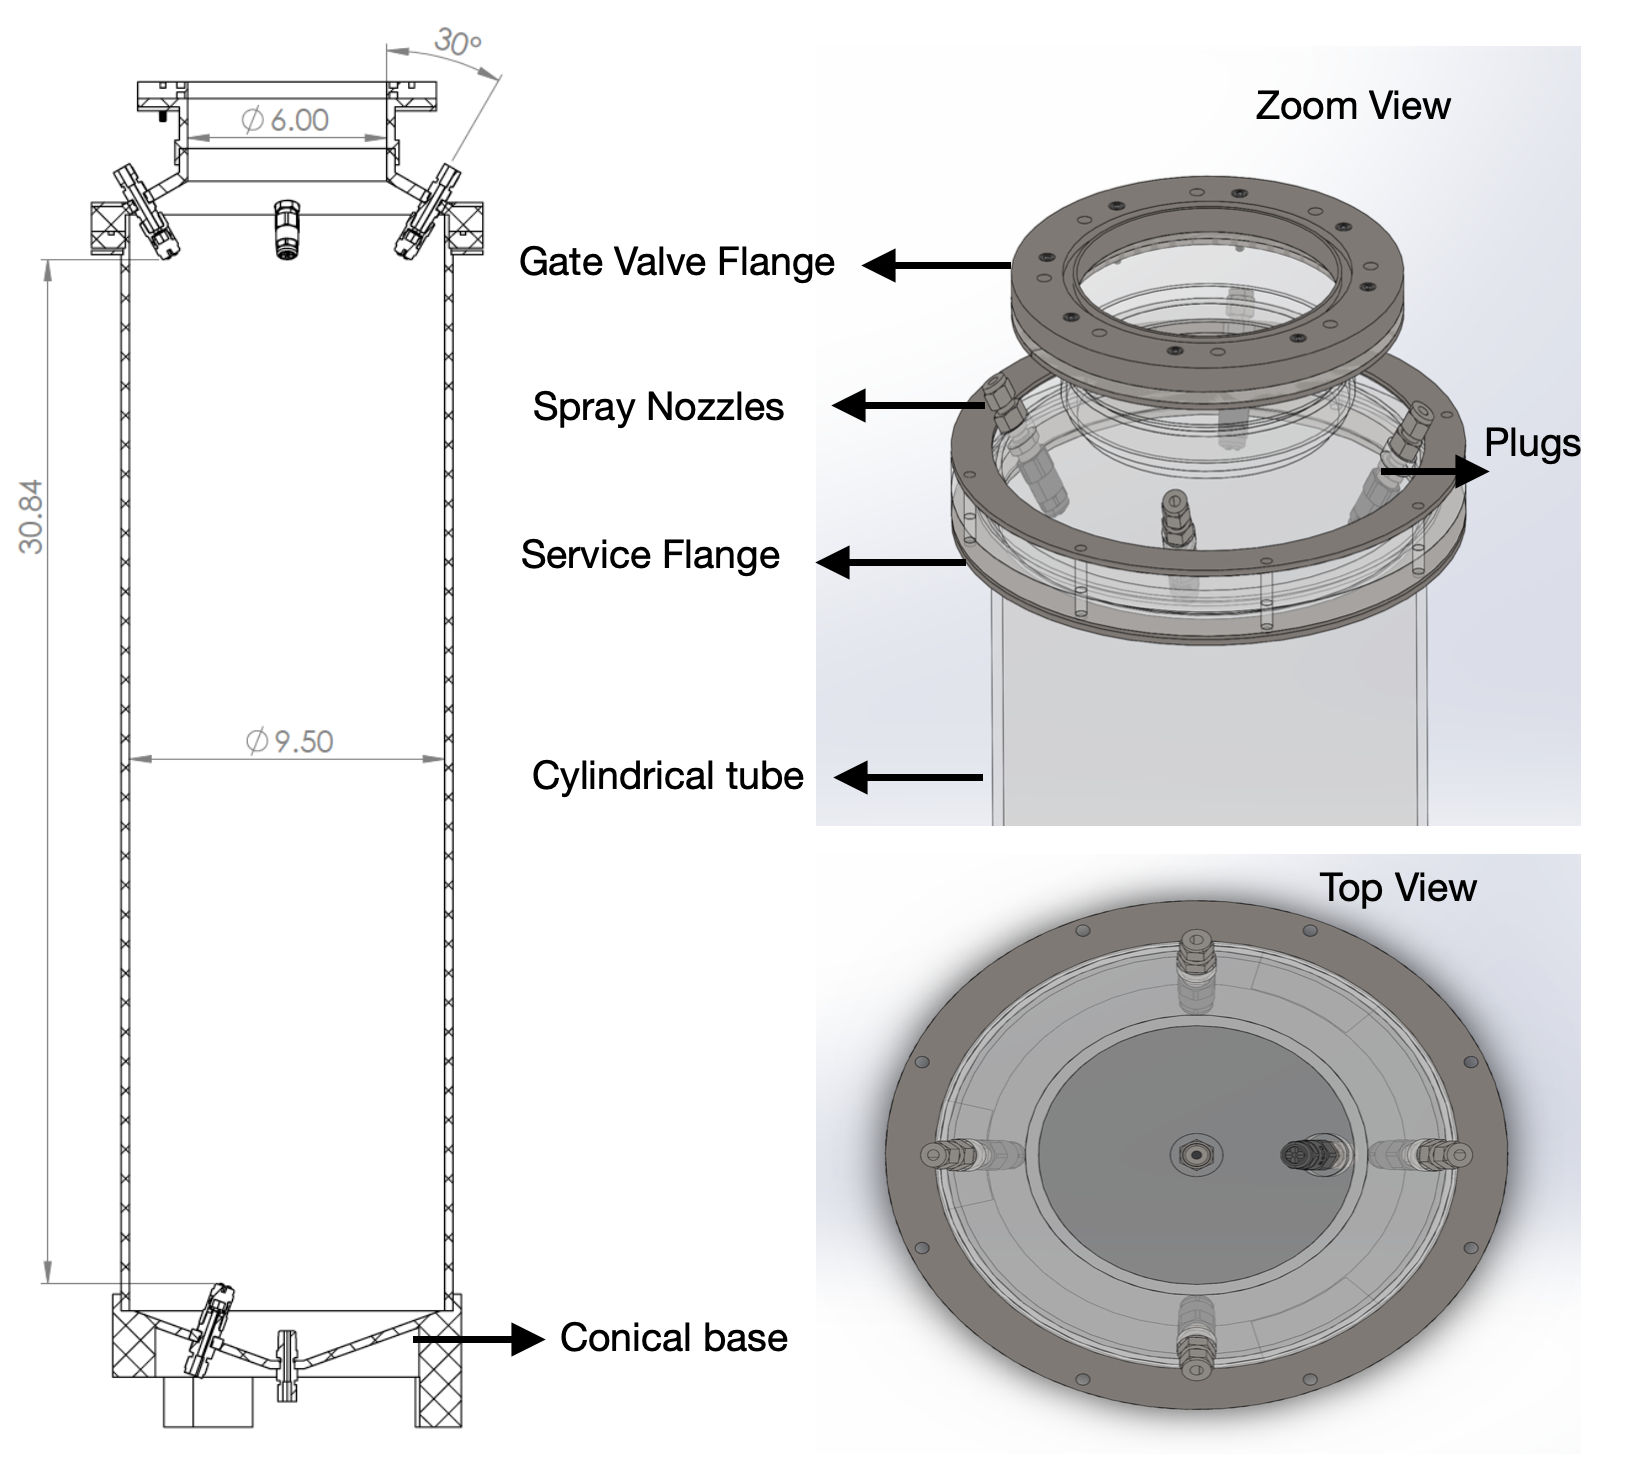
\includegraphics[width = 12cm, height=6cm ]{figures/SCV1}
  \caption{Source Cleaning Vessel}
  \label{fig:SCV}
\end{figure}

\section{ Definitions and Parts of the SCV}

\textbf{Cylindrical tube}: \\
It embodies the central part of the vessel that accommodates the source.\\
\\
Purchased From: Johnston industrial plastics limited\\
\\
Link:  \url{https://www.johnstonplastics.com}\\
\\
Dimension for the vessel: 9.50$''$(ID) x 0.25$''$(Thickness) x 30.84$''$(Length).\\
\\
Material: Cast Acrylic.\\
\\
**I will add a final drawing.\\
\\
\textbf{Plug rings}:\\
These are small rings to hold the bulkhead fittings.\\
\\
\begin{figure}[!htpb]
  \centering
  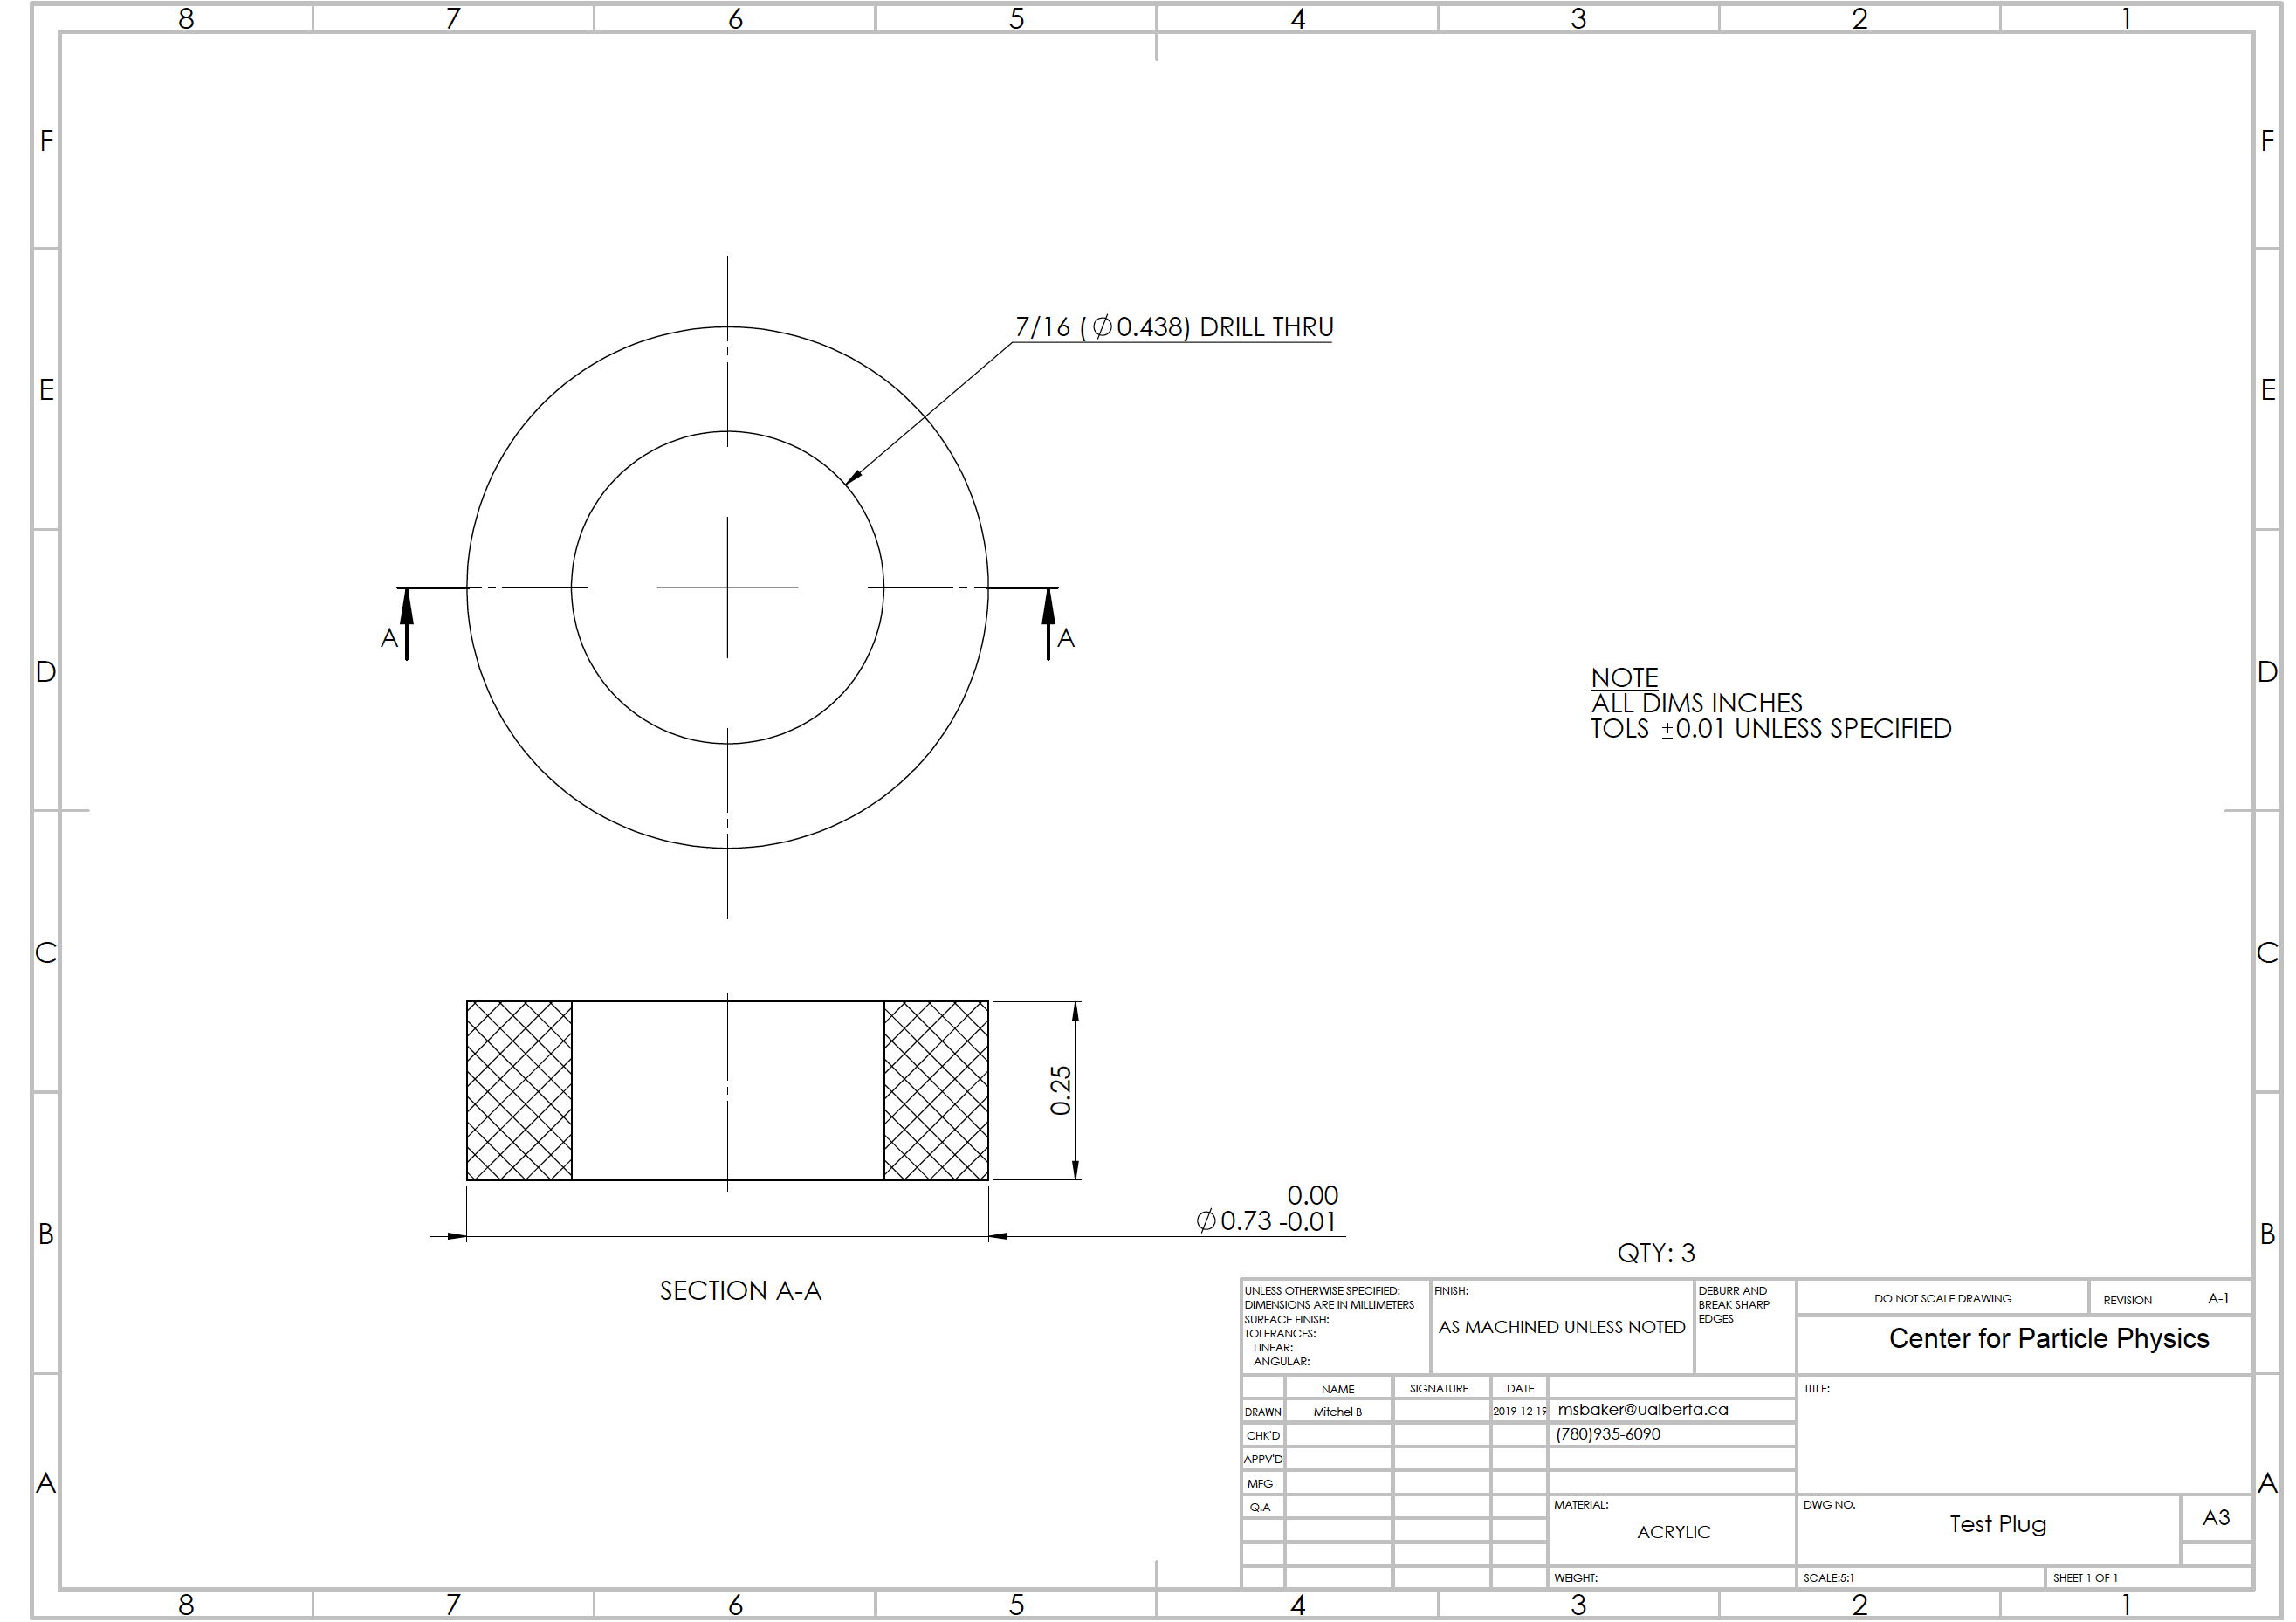
\includegraphics[width = 12cm, height=10cm ]{figures/plug}
  \caption{Drawing of the plug ring}
  \label{fig:plug}
\end{figure}
\\
Dimension: 0.43$''$(ID) x 0.25$''$(Thickness) x 0.73$''$(Length).\\
\\
Material: Acrylic ( Rod from physics workshop)\\
\\
/%\begin{figure}[!htpb]
 % \centering
  %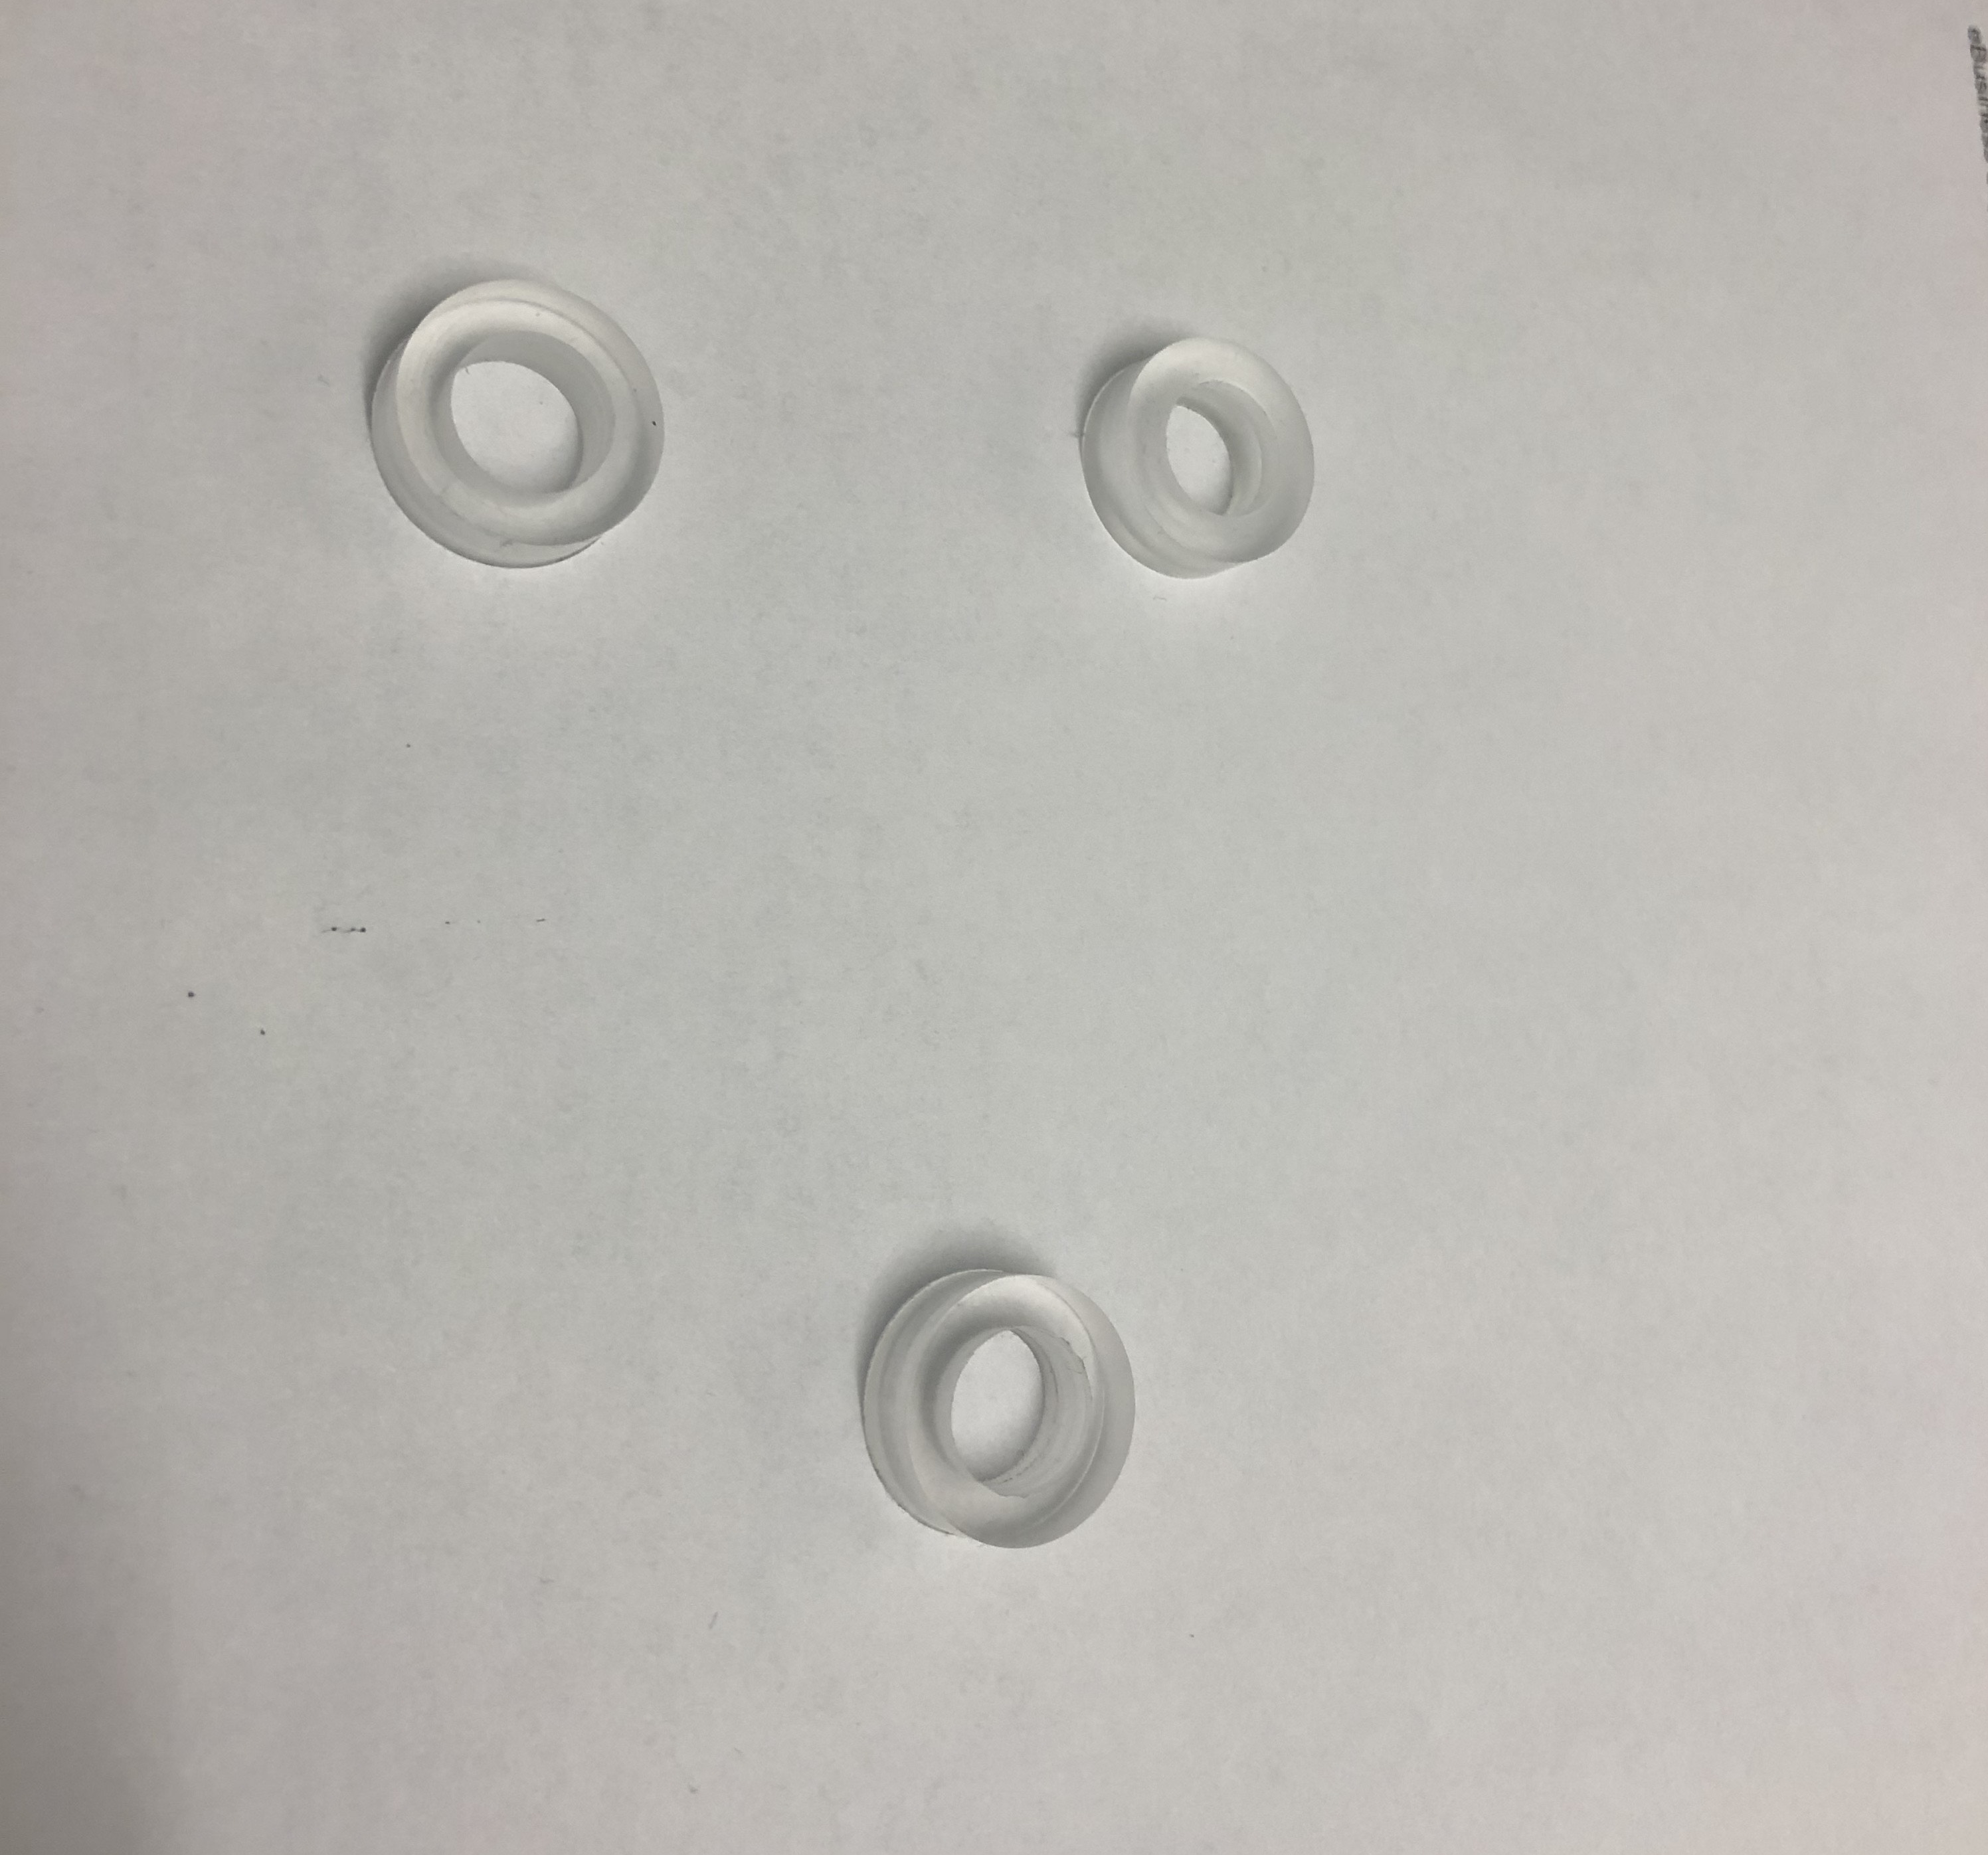
\includegraphics[width = 7cm, height=6cm ]{figures/plug1}
  %
  % 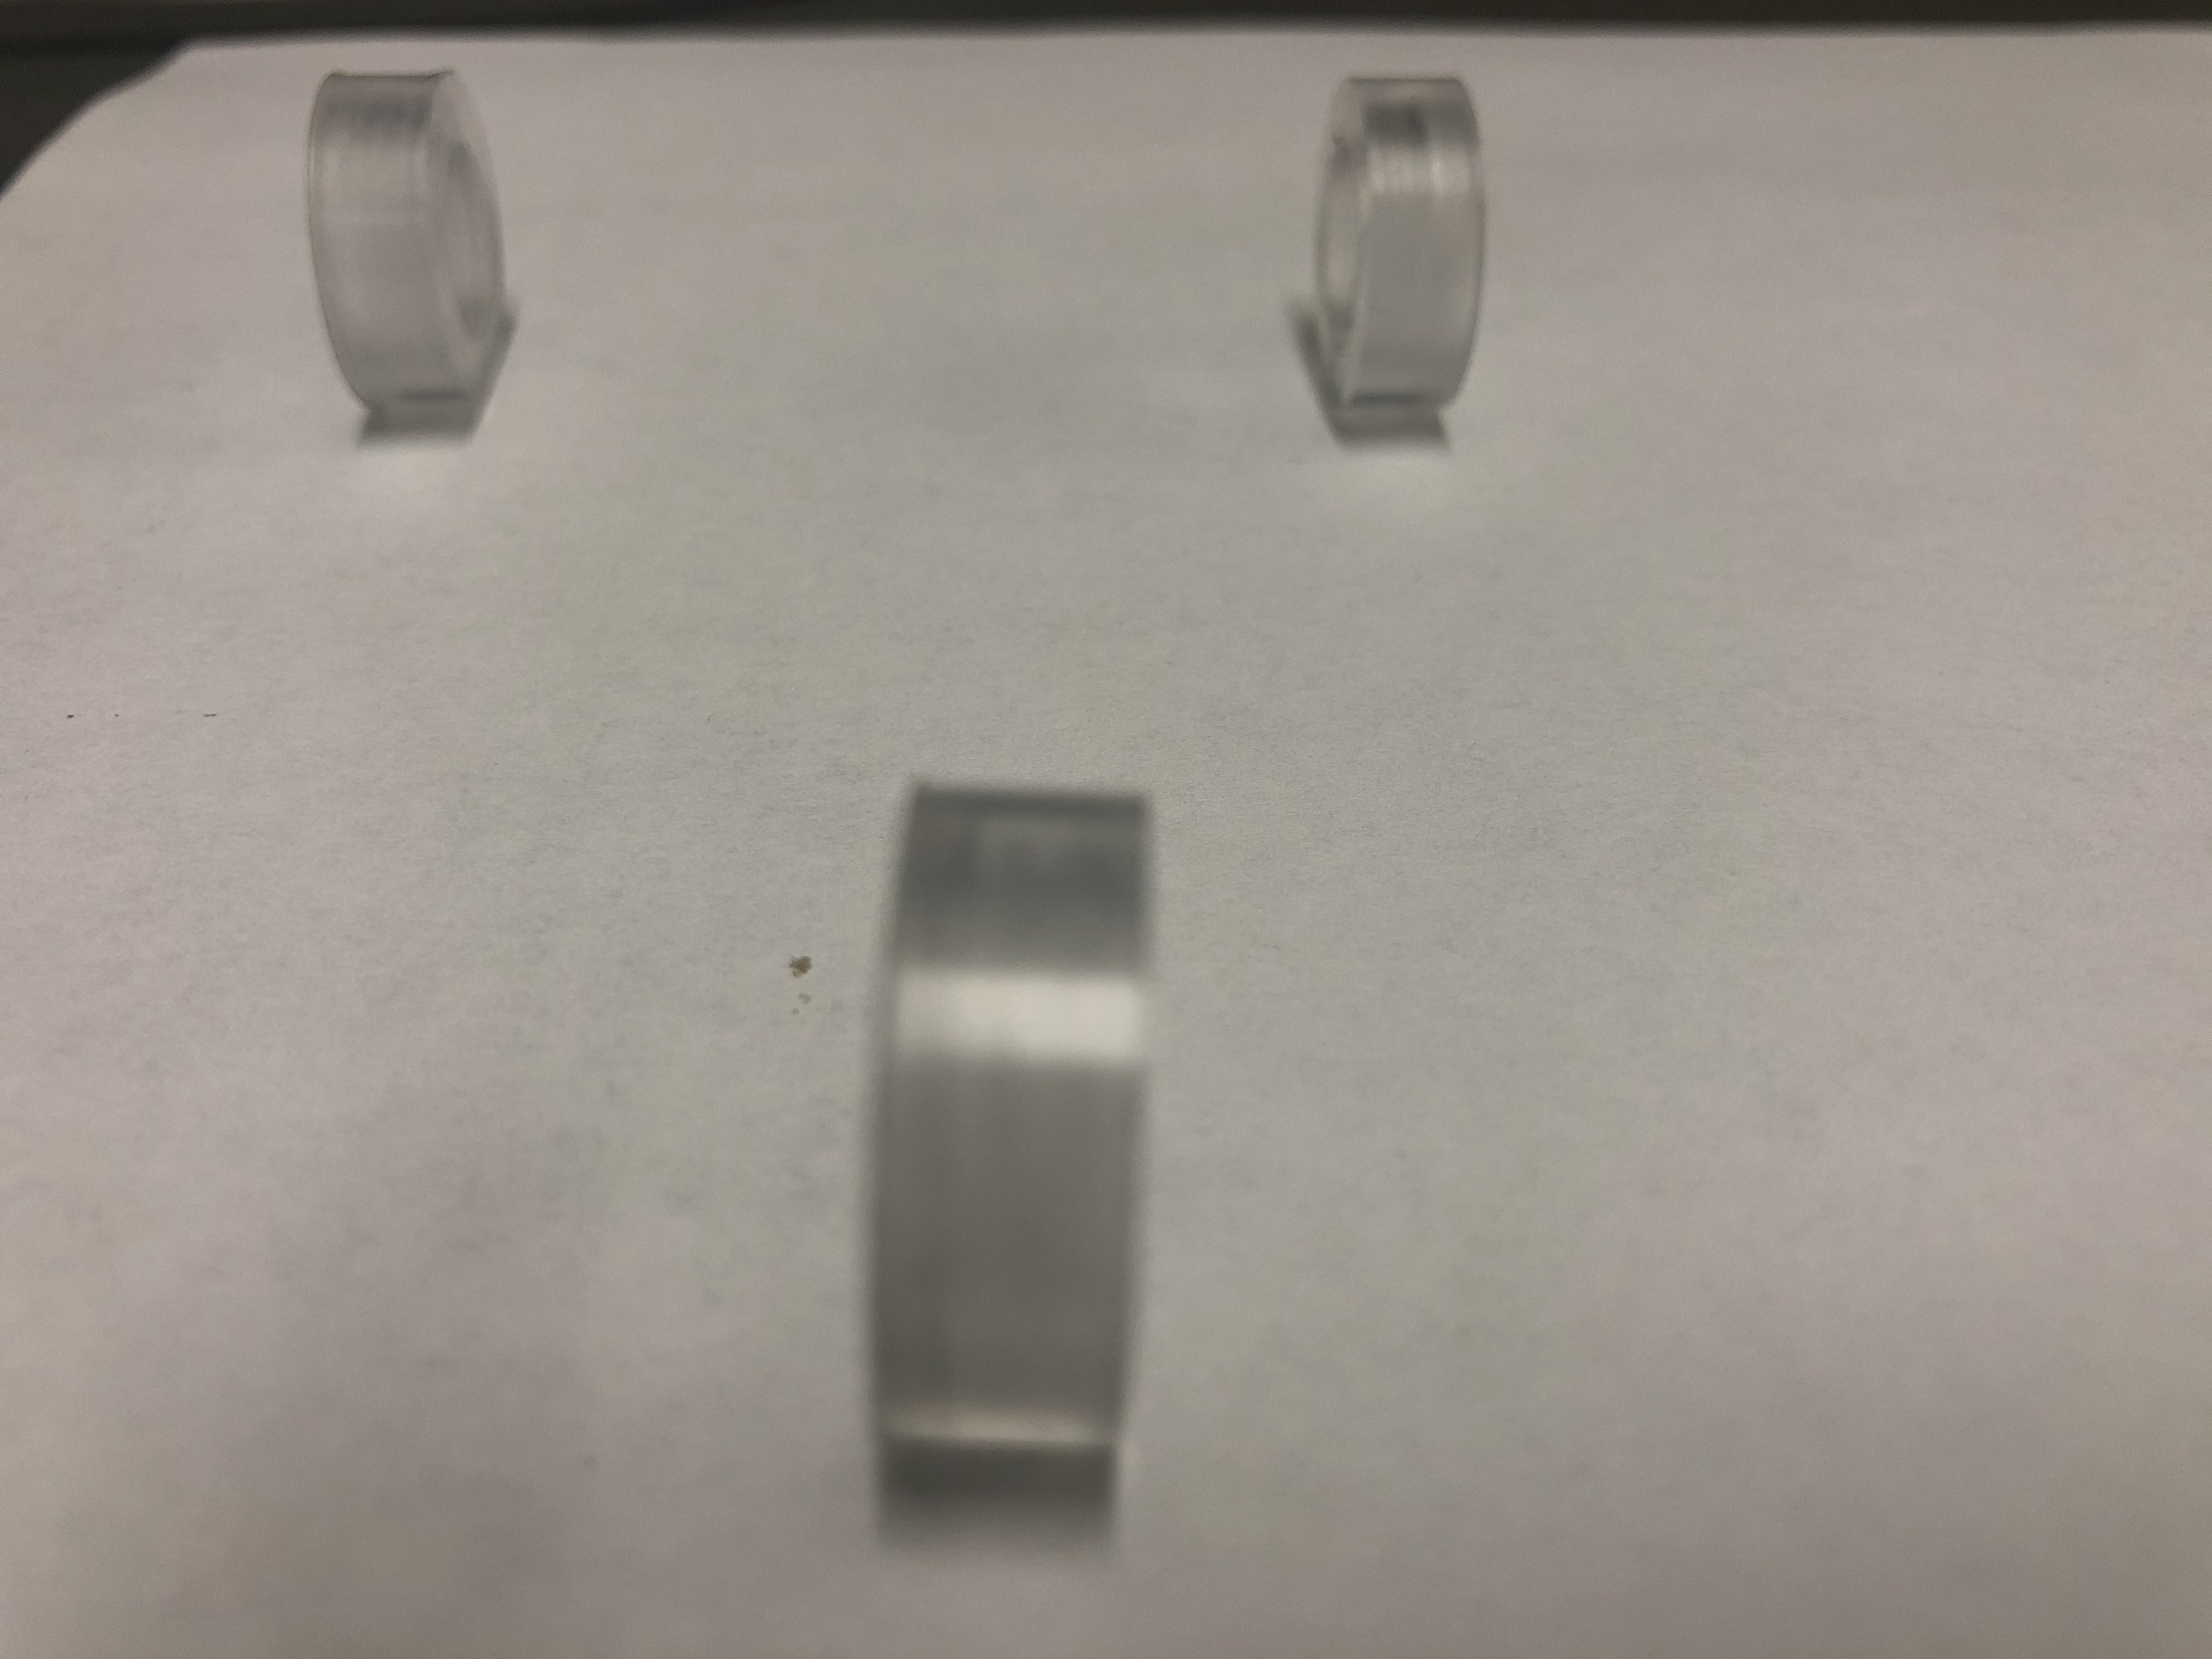
\includegraphics[width = 7cm, height=6cm ]{figures/plug2}
  %\caption{Plugs for bulkhead fittings}
  %l\abel{fig:plug1}
%\end{figure}
%
\\
\textbf{Flanges}:\\
Dimension for one of the service flange that we have machined for our test design:\\
\\
9.75$''$(ID) x 0.50$''$ (Thickness) x 11.80$''$(Length) \\
(I will add drawings of other flanges according to our final design once I got from Mitchel) .\\
\\
Material: Acrylic ( Acrylic sheet from lab L2-92)\\
\begin{figure}[!htpb]
  \centering
  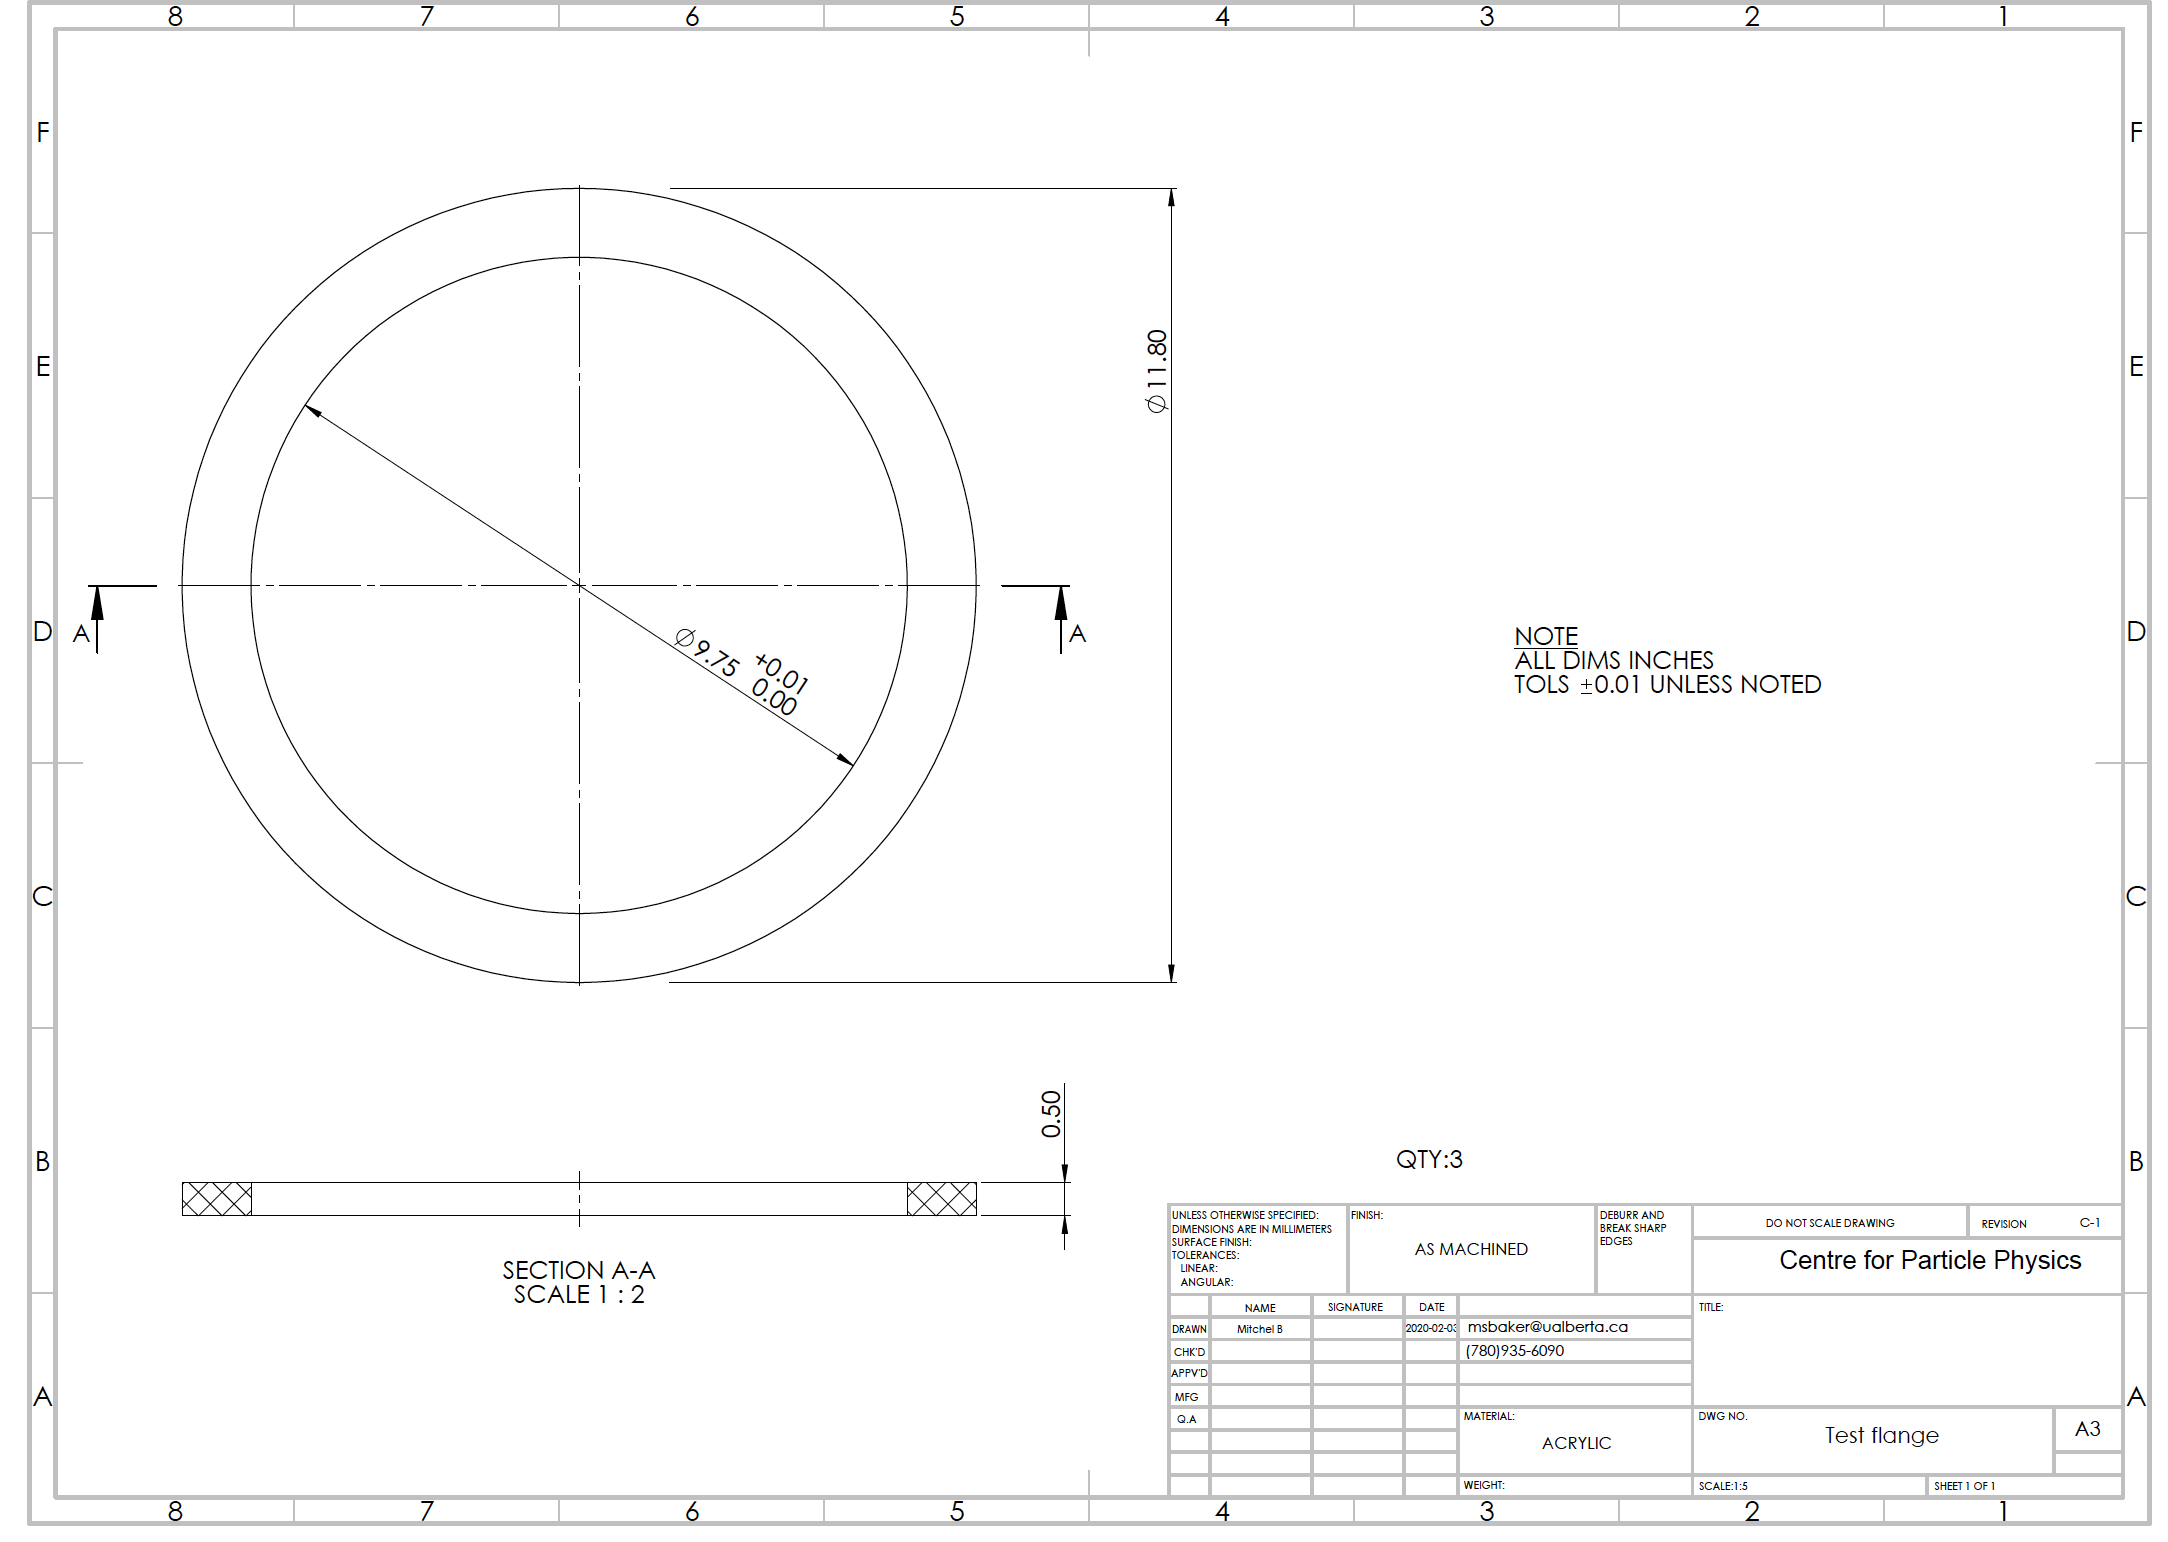
\includegraphics[width = 12cm, height=10cm ]{figures/flange}
  \caption{Drawing of the service flange}
  \label{fig:flange}
\end{figure}\\
\textbf{Conical Base}:
It is the bottom part of the vessel with a conical shape and provides a drainage port to collect LAB. The conical geometry allows the used fluid to drain from vessel.\\
\\
Material: Acrylic(Acrylic sheet from physics lab)\\
\begin{figure}[!htpb]
  \centering
  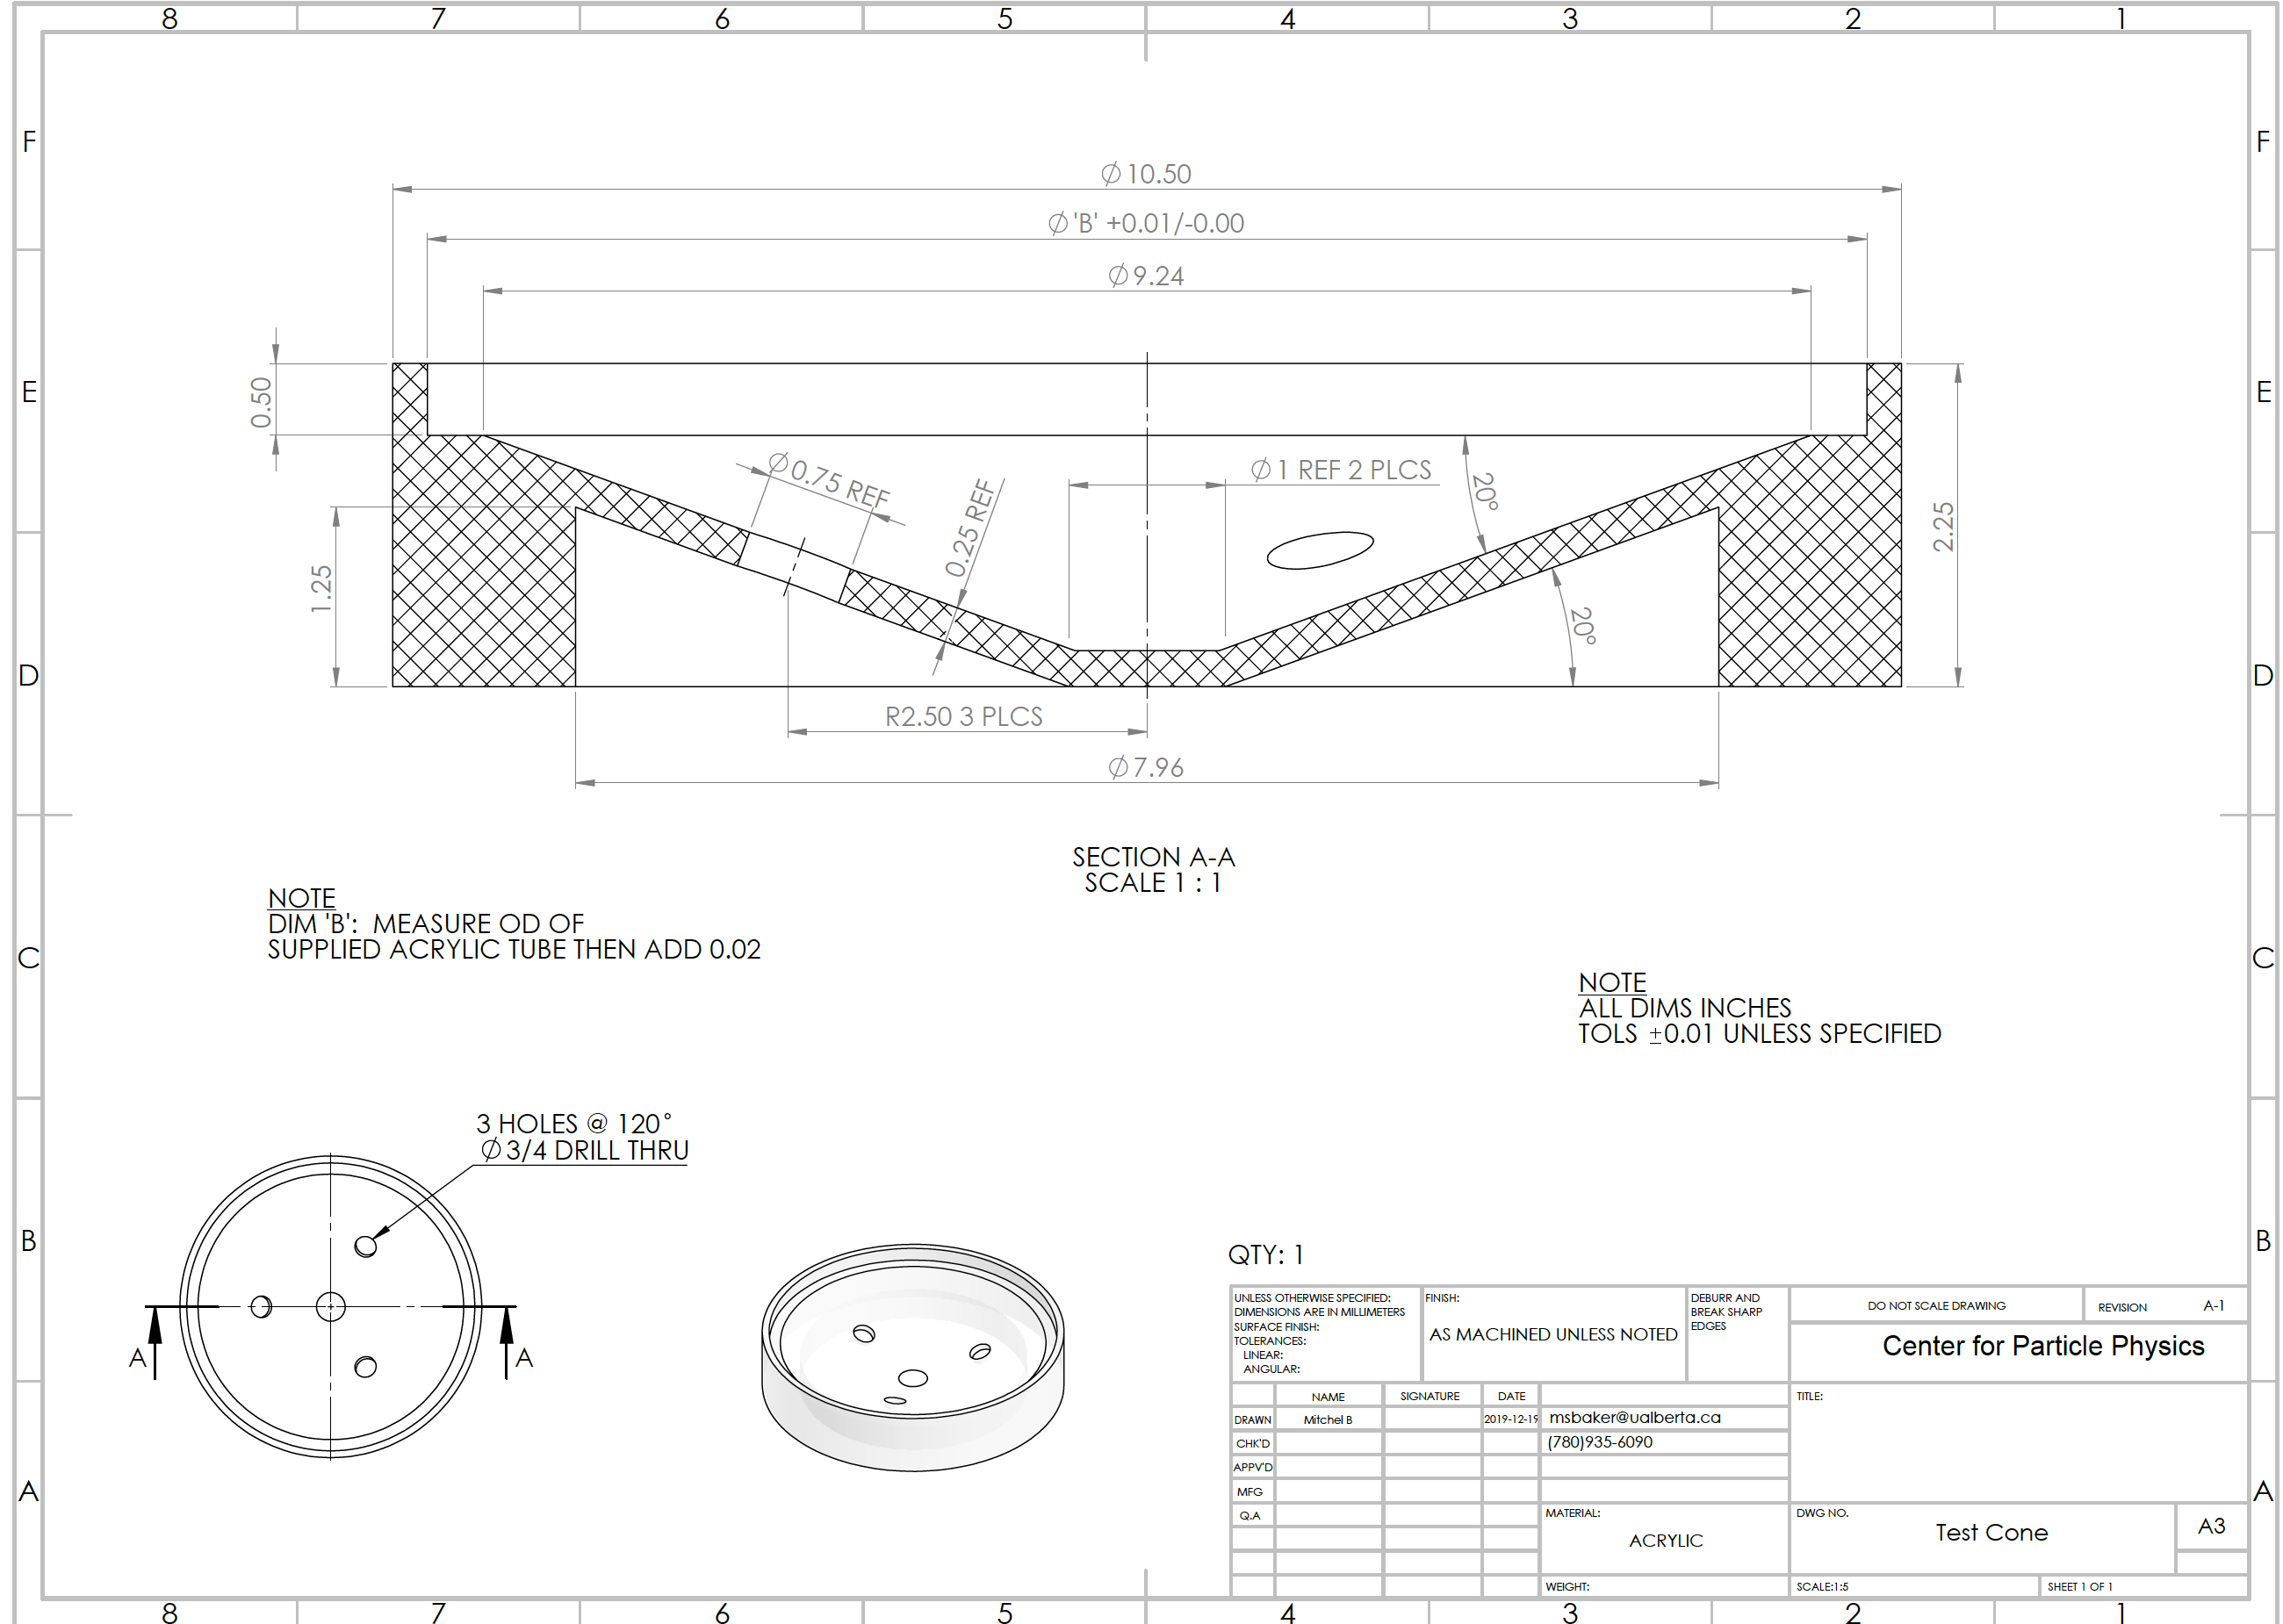
\includegraphics[width = 12cm, height=10cm ]{figures/base}
  \caption{Drawing of the Conical base}
  \label{fig:base}
\end{figure}
\\
\textbf{Spray Nozzles}:
The Spray nozzles are simple devices used to break apart a fluid flow into a spray pattern. It is one of the crucial parts of any cleaning system and needs to be chosen appropriately for effective cleaning. There are many variables that should be explored and investigated before the selection of suitable nozzles for any cleaning system. The variables are as follow:\\

\textbf{Dust particle size} \\                                              

\textbf{Spray drop size}\\

\textbf{Spray pattern}\\

\textbf{Spray angle}\\

\textbf{Operating pressure}\\

\textbf{Nozzle placement}\\
\\
Keeping in mind these requirements and after exploring all the variables according to the need of our system, we have chosen Full cone wide-angle ( 112 and 120 deg) hydraulic nozzles(Figure~\ref{fig:nzl})
\begin{figure}[!htpb]
  \centering
  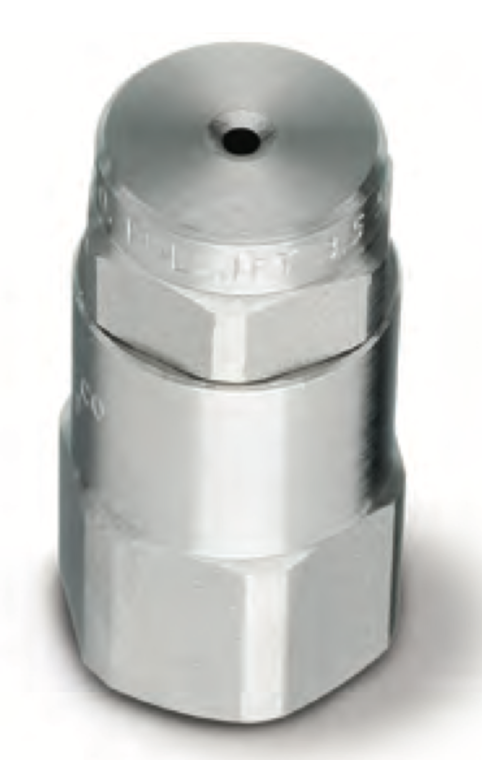
\includegraphics[width = 5cm, height=6cm ]{figures/nzl}
  \caption{Full cone wide angle nozzle}
   \label{fig:nzl}
\end{figure}
\\
Purchased from: Spraying system Canada ltd.(\url{ https://www.spray.ca}\\
\\
Material: Stainless steel 316\\
\\
Part Number: 1/4G-316SS4.3W \\
\\
In our case, we have placed nozzles on the top and bottom to rinse the source from all sides.\\
\\
\textbf{Bulkhead Fitting and O rings}: \\
\\
\textbf{Bulkhead fitting}:
It is an item that is designed to allow a connection through the wall of a container or vessel. The details of the fittings that we are using are follow:\\
\\
\begin{figure}[!htpb]
  \centering
  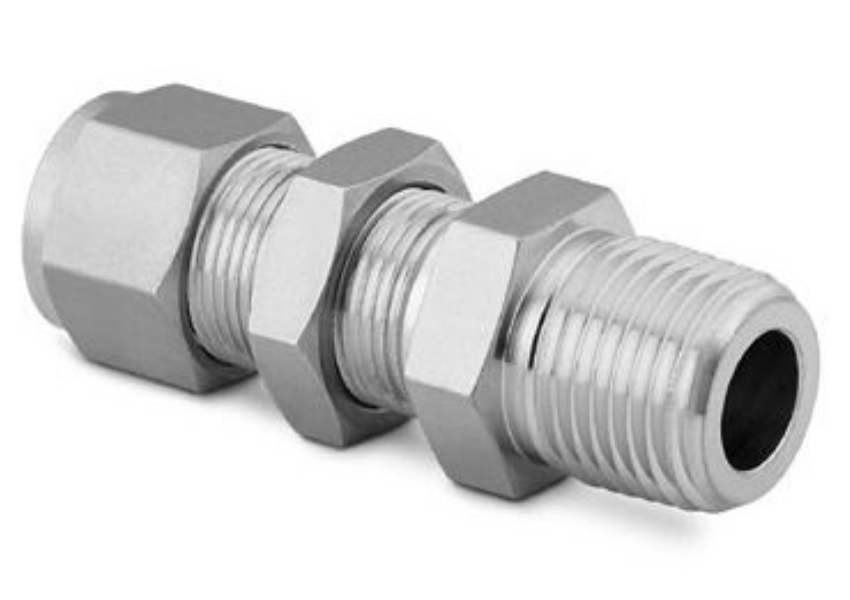
\includegraphics[width = 5cm, height=6cm ]{figures/ftng}
  \caption{Swagelog bulkhead fitting}
  \label{fig:ftng}
\end{figure}
\\
Purchased from: Swagelok Edmonton Valve and Fitting Inc.\\
\\
Material: Stainless steel 316.   \\                           
\\
Part Number: SS-400-11-4\\
\\
Connection type: Bulkhead Male Connector, 1/4$''$Tube OD x 1/4 $''$Male NPT\\
\\
\textbf{O rings}: 
\\
They are commonly used in sealing applications. In our operation we are using chemical resistant Viton Fluoroelastomer O-Ring with the bulkhead fitting for the airtight sealing.\\
\\
Purchased from: McMASTER-CARR.\\
\\
Material: Viton® Fluoroelastomer Rubber\\                                
\\
Part number: 9464K17\\
\\
\url{https://www.mcmaster.com}\\
\\
\begin{figure}[!htpb]
  \centering
  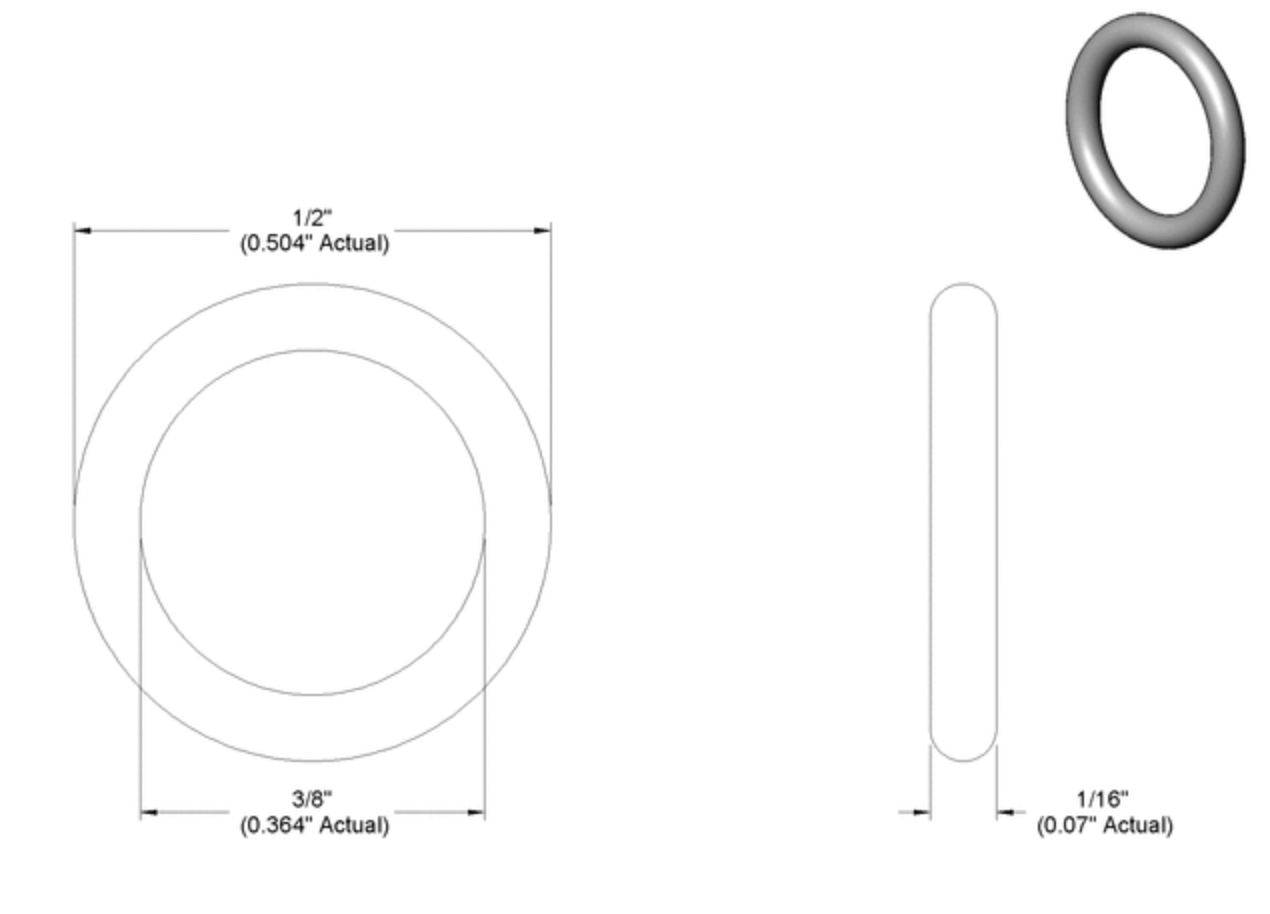
\includegraphics[width = 7cm, height=6cm ]{figures/oring1}
  \caption{Viton Fluoroelastomer O-Ring}
  \label{fig:oring}
\end{figure}
\\
\section{ Linear Alkyl Benzene (LAB) cleaning set up}
This setup is designed to provide clean LAB for the cleaning of SNO+ sources . The complete unit consists of different parts such as pump, filters, pulsation dampener, piping system, fitting and cart.  LAB is noncorrosive (SDS) hence doesn’t demand any specific storage but from previous experience and observations, it is recommended to use stainless steel and PTFE wetted parts only, LAB is known to swell and degrade elastomers over time. \\
\\
\textbf{Parts of LAB set up}:\\
The details of all the parts associated with the unit are as following:\\
\\
\textbf{Piping system and fittings}:\\
\begin{itemize}
\item  1/2$''$ 316 stainless steel tubing with a wall thickness of 0.049$''$: \url{https://www.mcmaster.com/89785k845}.
\end{itemize}

The list of fittings includes:\\
\begin{itemize}
\item Four hose connections (1/2$''$ to 3/8$''$): SS-815-6: \url{ https://www.swagelok.com/en/catalog/Product/Detail?part=SS-815-6}
\end{itemize}

\begin{itemize}
\item Four 1/2$''$ unions: SS-810-6 
\end{itemize}

\begin{itemize}
\item Five 1/2$''$ MNPT to Female Swagelok Connect: SS-810-1-8 
\end{itemize}

\begin{itemize}
\item One 1/2$''$  MNPT to Male Swagelok connect: SS-8-TA-1-8 
\end{itemize}

\begin{itemize}
\item One 3/4$''$ MNPT to Male Swagelok connect: SS-8-TA-1-12
\end{itemize}

\begin{itemize}
\item Three   1/2$''$ tees, and one  1/2$''$ tee with a 1/4$''$ connection: SS-810-3: 
\end{itemize}

\begin{itemize}
\item Stainless Steel Swagelok Tube Fitting, Male Tube Adapter, 1/4 $''$ Tube OD x 1/4 $''$ Male NPT: SS-4-TA-1-4
\end{itemize}

\begin{itemize}
\item Stainless Steel Swagelok Tube Fitting, Male Tube Adapter, 1/4 $''$  Tube OD x 1/8$''$ Male NPT: SS-4-TA-1-2 
\end{itemize}

\begin{itemize}
\item Stainless Steel Swagelok Tube Fitting, Reducing Union Tee, 1/2 $''$  x 1/2 $''$  x 1/4 $''$ Tube OD: SS-810-3-8-4
\end{itemize}

\begin{itemize}
\item One pressure gauge. It has a range from 0 to 100 psi: PGI-63C-OG100-LAQX
\end{itemize} 
\textbf{Valves}: All valves are manufactured by Swagelok and were purchased through Edmonton Valve and Fitting. The list includes:\\
\\
\begin{itemize}
\item Two 3-way 1/2 $''$ valves:SS-45XS8: 
\end{itemize}

\begin{itemize}
\item Two 1/4 $''$valves for the drain ports on the filter housings: SS-42GS4
\end{itemize} 
\textbf{Pump, Filter, and Pulsation Dampener}\\
\\
\textbf{Air Operated Diaphragm Pump}\\
The choice to go with an pump was based on experience from similar wash systems built. Additionally, it is cost effective compared to other pumps and does not require electricity to operate. The Air Operated Double Diaphragm  pump was manufactured by Sandpiper. It has a housing made out of aluminum and stainless steel and all wetted materials are made up of stainless steel and PTFE. \\
\begin{itemize}
\item \url{https://www.sandpiperpump.com/products/standard-duty-ball/s05-metallic}
\item \url{https://www.mcmaster.com/41655k27}\\
\end{itemize}

\begin{figure}[!htpb]
  \centering
  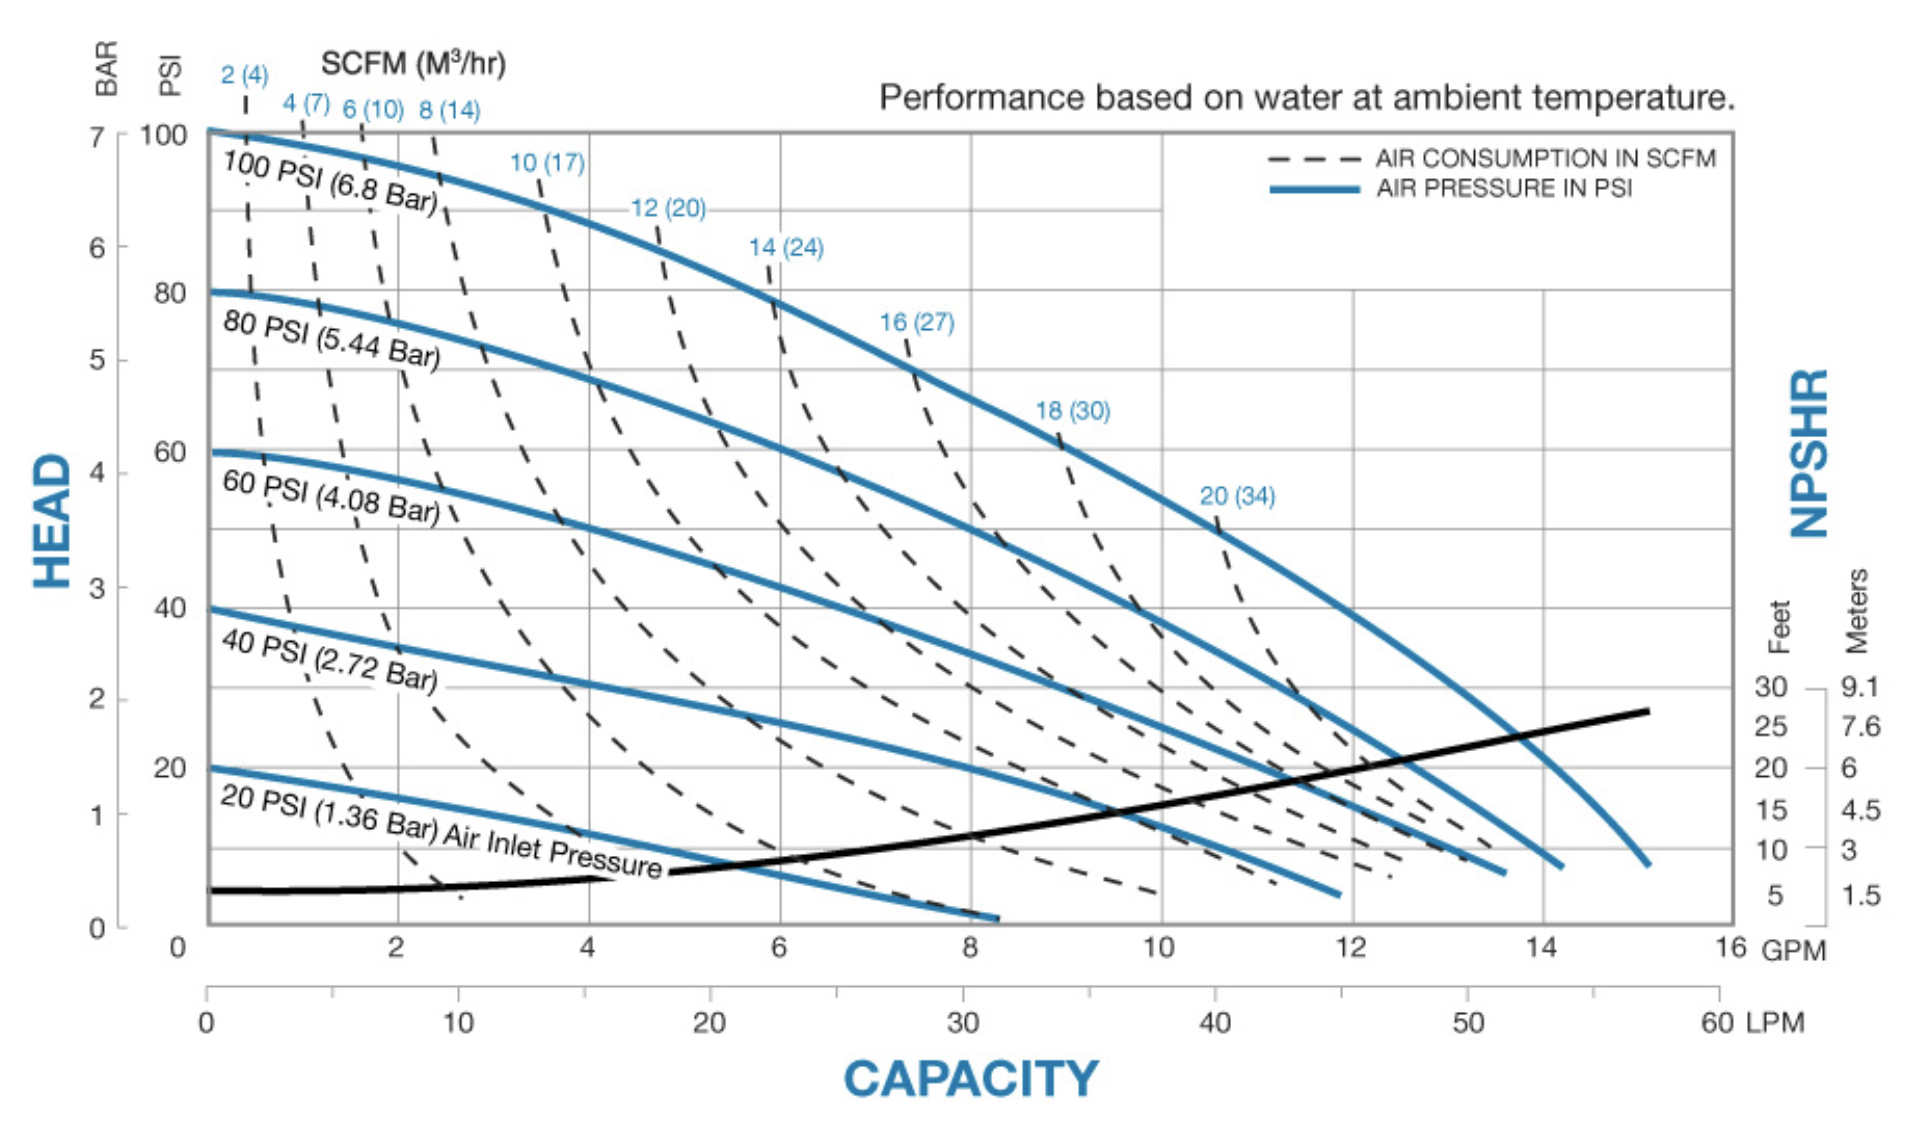
\includegraphics[width = 12cm, height=10cm ]{figures/curve}
  \caption{Performance curve}
  \label{fig:curve}
\end{figure} 
 
The diaphragm and check valve balls are made out of PTFE and the maximum air pressure the pump can handle is 125 psi .The purchased air regulator has an air flow of 53 cfm at 100 psi and has a maximum pressure of 140 psi.\ The performance curve of the pump is shown in Figure~\ref{fig:curve} \\
 \\
 \textbf{Filter Housing}\\
To not impede the flow rate of the fluid, 20$''$ long filter housings have purchased and to accommodate the filters, two stainless steel Shelco 20$''$  Filter housings have procured through CPS Filtration. They are designed for a 20$''$ (length) and 2.5$''$  (diameter) filter cartridge.\\
\url{ https://cpsfiltration.com}\\
\\
\textbf{Filter Cartridge}\\
The cartridges are made up of 20$''$ PTFE membrane with polypropylene core material and Teflon (PTFE) gaskets.  The filter cartridges were purchased through CPS filtration and  are manufactured by American Melt Blown and Filtration. They have a maximum differential pressure of 45 psid (pounds per square inch differential).\\
\url{  https://cpsfiltration.com}\\
\\
\textbf{Pulsation Dampener}\\
One disadvantage to using an AODD pump, is that the pressure of the fluid is periodic, since the pump pulses due to the diaphragms opening and closing. The pulsation dampener is designed to correct this by “smoothing” out the pulsations of the fluid, so that a steady flow is achieved. The pulsation dampener was manufactured by Blacoh Fluid Control (\url{https://www.blacoh.com/home.aspx}) and  model CT3120T was purchased through Natpro. The pulsation dampener is made out of stainless steel with a PTFE bladder.  It holds a maximum operating pressure of 300 psi at \ang{20} C. The pulsation dampener must be charged to 80$\%$ of the head pressure to ensure maximal dampening.\\
\\
\textbf{Cart Framing}\\
Made out of 1.5” T-Slot Aluminum extrusions (manufactured by 8020) due to its ease of assembly and versatility. 
\url{https://8020.net/?SID=og9et35936f61t6v13tron8os1}
\url{https://www.mcmaster.com/47065t103}    \\
\begin{figure}[!htpb]
  \centering
  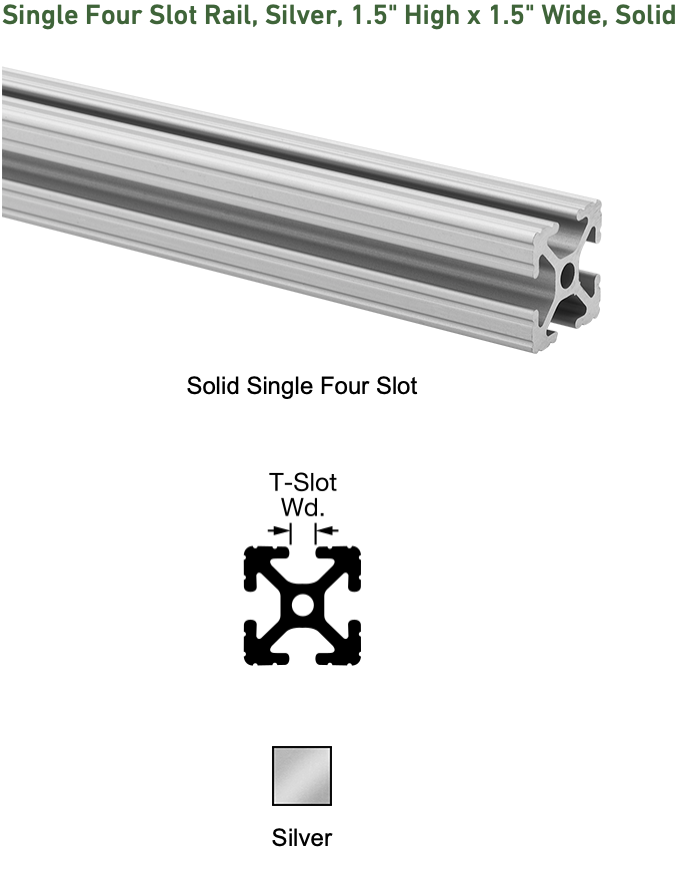
\includegraphics[width = 7cm, height=6cm ]{figures/frame}
  \caption{Aluminum cart framing}
  \label{fig:frame}
\end{figure}

\textbf{Spill Tray}
\begin{itemize}
\item Made out of polypropylene:\url{https://www.usplastic.com/catalog/item.aspx?itemid=125655}
\item Dimension: 24$''$x24$''$x4$''$
\item Can hold 37 litres of fluid\\
\end{itemize}


\section{Appendix}
Important links for Spray nozzles and related literature :\\
\\
\url{https://www.spray.ca}\\
\\
\url{https://www.spray.com/-/media/DAM/Sales-Materials/b/B652A_Spray_Technology_Dust_Control.pdf}\\
\\
\url{https://www.spray.ca/spray_nozzles/full_cone_fulljet_nozzles.aspx}\\
\\
\url{https://www.spray.ca/literature/literature_cat75.aspx}\\
\\
\url{https://www.spray.ca/Assets/SPRAY/Cat75HYD_US_B.pdf}\\
\\



 















\chapter{Source Cleaning Apparatus Manual}
\section{Purpose}
This document describes the necessary information and standard procedures that \textbf{must} be followed for the operation and handling of  the source cleaning vessel. In case a part or step of this procedure is not clear or a statement in the procedure contradicts the state of experiment, do not continue with the process. Contact the calibration coordinator and detector manager and get permission to proceed 
\section{Definitions}
\textbf{Cleaning Module}: An apparatus that can be attached directly to the source tube gate valve that sprays a flow of LAB directly onto a source to facilitate cleaning. The set up allows to draw LAB for testing .\\
\\
\textbf{Source Connector}:A device by which a source may be temporarily connected to an umbilical while also allowing bre optic or electrical connections.\\
\\
\textbf{Umbilical Retrieval Mechanism(URM)}:The device in which the umbilical is stored
in preparation for deployment that also includes drive mechanisms for the central rope and umbilical to facilitate vertical movement of sources.\\
\\
\textbf{Source Tube}: A tube connecting to the bottom of the URM with a bellows below that terminates on a gate valve that connects to a nipple assembly on the UI when the URM is in a position ready for deployment.\\
\\
\textbf{Umbilical}: A length of Tygothane tubing containing an optical fiber and five electrical wires to which calibration sources are attached for deployment in the AV.\\
\\
\textbf{Boil Off Nitrogen}: Nitrogen sourced from a cryogenic nitrogen dewar that is installed in the Utility drift and is transferred  to the DCR by way of copper conduit (high pressure) or from the international dewar (low pressure). The pressure of the high pressure nitrogen boil off  for purging purposes must be regulated using the gas board in the DCR to less than 20 psi. ( @ Ryan Reference to the relevant procedure required )\\
\\
\textbf{Linear Alkyl Benzene(LAB) cleaning set up}: This setup is designed to clean the LAB. The complete unit consists of different parts such as pump, filters, pulsation dampener, piping system, fitting and cart.\\
\section{Description of the Cleaning Module}
The cleaning module consists of a  31.78" long cylindrical tube with 9.50" interior diameter. Inlet and outlet gas connections are supplied to allow nitrogen flushing of the module independent of the URM system. Four LAB sprayers near the top of the cleaning module provide a stream of LAB to actively rinse the source. The flange at the top of the source allows  to connect the cleaning module to the gate valve at the bottom of the URM source bellows. A cart with a jack is provided to move and lift the cleaning module into position, and provide a clean working surface for source work.
\begin{figure}[!htpb]
  \centering
  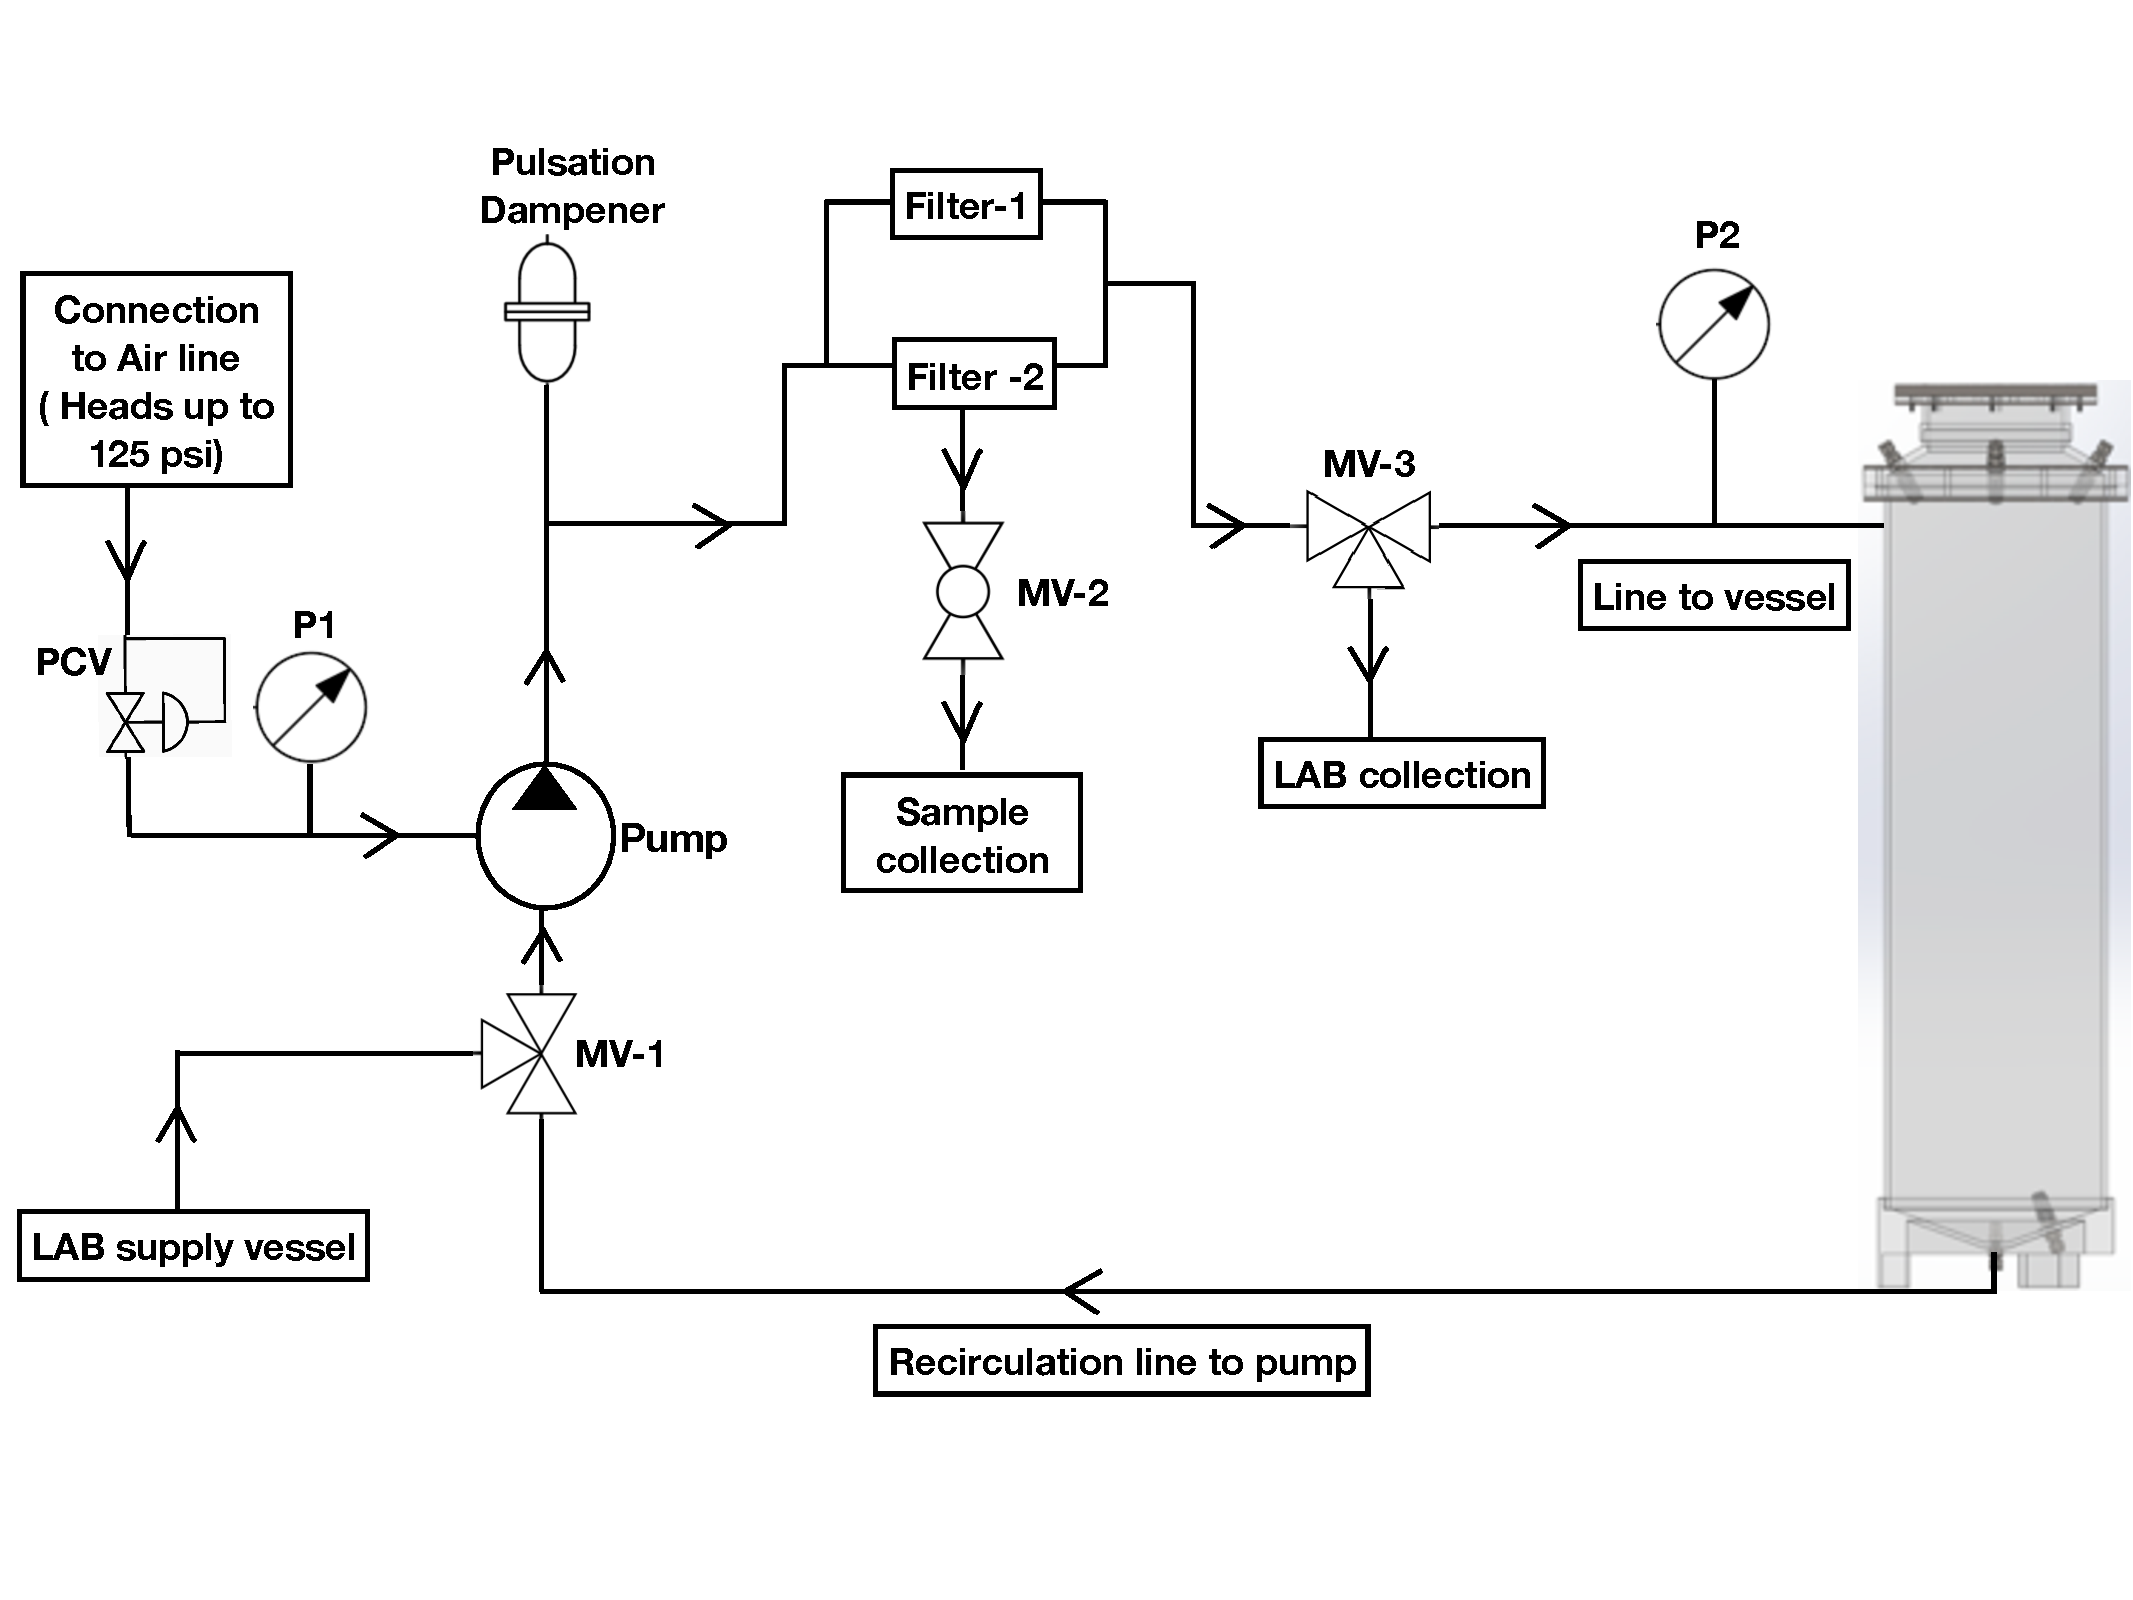
\includegraphics[width = 14cm, height=14cm ]{figures/LAB_3}
  \caption{Line Diagram of the LAB cleaning set up}
  \label{fig:SCV}
\end{figure}
\\
\section{Important points and prerequisite}
Before commencing any activities related to the source cleaning vessel and LAB set up, the designated people should follow these steps:
\begin{enumerate}
\item The Safety Data Sheet (SDS) must be thoroughly reviewed each time when handling LAB. Permission from the detector manager must be obtained in writing.
\item All person must be equipped with required PPE ( Nitrile gloves, masks, safety glasses, head cap) before the starting of any procedure and change them as required.
\item The vessels must be handled with fresh, clean gloves and face masks must be used by the individuals involved in the activity.
\item  When moving the vessels, there must be at least three people present: one will be the “dirty” person, the other two “clean”.
\item The “dirty” person must keep an eye on the clean persons at all time and ensure that the clean persons not get in contact with any unclean surface.  If in any case it happen then instruct them to change their PPE.
\item Every piece of equipment that will receive parts or need additional items like wrenches, screw drivers etc. need to be set up first (checked, cleaned and put in appropriate location etc) before the vessel is moved, or used.
\item The receiving parts must be thoroughly cleaned with Ultra Pure Water(LPW). 
\item No clean part should be touched without clean gloves and masks on.

\end{enumerate}


\section{Procedures}
The following procedures must be done within the deck clean room and all necessary protocols must be followed. It is assumed that the operator is to perform all operations using latex gloves in addition to standard Personal Protective Equipment (PPE). Dust counts should be monitored prior to operations involving opening the  URM source tube or exposing a source. If the dust count appears to be high, the DCR should be cleaned and the intended procedure should be suspended. All procedures listed here should be completed with the participation of a calibration expert.

\subsection{Connecting the URM to the UI}

\subsection{Disconnecting the URM from the UI}

\subsection{Using the Source Connector}

\subsection{Attaching a Source to the Umbilical}\label{ss:sourceattach}

 The instructions below presuppose that the source is not connected to the umbilical. Note that the following only applies to the North side URM as the South side URM will have the Cherenkov source permanently attached to its umbilical. Sources of LAB, and boil off nitrogen should be procured before attempting the following procedure.

\begin{enumerate}
\item Begin with the source in the cleaning module
\item Start the flushing the cleaning module with N$_{2}$ 
\item Move the URM back from the UI over the working area West of the UI
\item Position the cleaning module cart under the URM
\item Close the URM cover gas bag and start actively flushing the URM with N$_{2}$
\item Open the gate valve and lower the source connector until it can reach the source.
\item Connect the source to the umbilical via the source connector. 
\item Raise the source into the source tube
\item Connect the cleaning module to the source tube gate valve
\item Make connections (Can be done by any one of the two clean person) for the  airline fitting at the specified port on the  LAB cleaning set up for starting the pump.
\item Check the connection for the inlet of LAB cleaning set up with LAB supply vessel (Ensure that the vessel  is filled with the minimum level (approximately 10 litre) of LAB required for the cleaning procedure ).
\item Set the bottom MV1  toward the injection line and the MV3 toward  line to the vessel.
\item Start the pump by providing the pressure from the Air line ( Maximum upto 125 psi, Pressure can be controlled by the pressure control valve) and allow LAB to flow in the LAB cleaning set up.
\item Wait until an adequate amount (When a 2/3 volume of the bottom conical part in the source cleaning vessel is filled with the LAB) of LAB is pumped in the LAB cleaning set up.
\item Once the adequate amount of LAB is filled  in the LAB cleaning set up then stop the pump and set the MV1 toward the recirculation line.
\item Turn on the pump again and allow LAB to flow in the LAB cleaning set up.
\item While the LAB flowing  lower the source through the LAB stream. The source should be  raised and lowered through the spray to remove surface contamination. The initial rinse should continue until the source (and the source connector) are clean.
\item Monitor the O$_2$ levels in the URM to validate the cover gas viability. The URM radon levels should also be monitored directly using the RAD7. The cover gas should be considered viable after the measured radon levels are consistent with zero. Once the cover gas is deemed viable the N$_{2}$ flush can be terminated and the cover gas bags can be opened to the URM. 
\item Take a sample to be submitted for analysis. To collect samples, set the manual MV2 at the On position, after collecting samples set the valves again at the off position.
\item Repeat spraying the source with LAB as above until the source get sample analysing . Allow the source to sit in the LAB for some time (order of a week) periodically draining the LAB, submitting samples for analysis . Record the status of the LAB cleanliness for each sample preparation (need to define a quantifiable cleanliness criteria)
\item Once the LAB cleanliness criteria is reached (TBD) the source should be raised into the source tube, the gate valve closed and the cleaning module disconnected from the gate valve. 
\item Move the URM back to the UI and reconnect the gate valve to the nipple assembly on the UI
\item Once the cleaning operation is complete, then the remaining LAB from the processing lines can be flushed out from the LAB cleaning set up by using the “dump” line. 
\item To do this, again turn off the pump, set the MV3 to the “dump” line where it should be connected to a container to accumulate the fluid. 
\item Then turn the pump on and pump until there is no more fluid exiting the dump line. Note that this will remove the majority of the fluid, but there will always be some fluid left within the process lines. 
\item Turn off the pump by stopping the pressure from the Air line at the specified port. 
\end{enumerate}

\subsection{Cleaning a Source Prior to Use}
Here, the minimum guidelines for cleaning a source should be set out. Each group should have their own specific cleaning instructions which should be compiled with this document. However, prior to use each source should
\begin{enumerate}
\item be inspected by a designated person to look for signs of corrosion or damage to the source
\item be wiped down using ultra pure water to initially pick up surface contaminants
\item be wiped down with an alconox mixture to futher remove surface contaminants
\item be wiped down with ultra pure water again to remove the alconox
\end{enumerate}

\subsection{Detaching a Source from the Umbilical}
Required for this procedure is a storage module for the source. This module should be connected to a pump/purge system to keep the source in a nitrogen environment between uses.
\begin{enumerate}
\item Ensure that the source storage module is available for use on the source cart.
\item Disconnect the URM from the UI.
\item Move the URM back to the working area and place the source cart in the working area
\item Disconnect the URM cover gas bag and flush nitrogen through the URM.
\item Open the source tube gate valve over the working surface of the source cart.
\item Lower the source to the working surface of the source cart.
\item Disconnect the source from the umbilical at the source connector.
\item Place the source in the storage module. Close the storage module and pump nitrogen into the storage module.
\item If a new source is not to be immediately connected to the umbilical, retract the source connector back into the URM source tube and close the gate valve. Continue the URM purge until O$_{2}$ monitor and RAD7 values are below established thresholds before the cover gas bags are reconnected. 
\item If a new source is to be reconnected refer to Section \ref{ss:sourceattach}.
\end{enumerate}






\end{document}
